\documentclass[degree=bachelor,tocarialchapter,table,xcdraw]{thuthesis}
% 在\documentclass中加入了 ,table,xcdraw 解决了用于表格颜色填充的宏包 \usepackage[table,xcdraw]{xcolor} 导致的xcolor不同参数重复声明的问题

% 选项
%   degree=[bachelor|master|doctor|postdoctor], % 必选,学位类型
%   language=[chinese|english], % 可选(默认:chinese),论文的主要语言
%   secret,                % 可选(默认:关闭),是否有密级
%   tocarialchapter,       % 可选(默认:关闭),章目录中使用黑体(这项表示同时打开下面两项)
%   tocarialchapterentry,  % 可选(默认:关闭),单独控制章标题在目录中使用黑体
%   tocarialchapterpage,   % 可选(默认:关闭),单独控制章页码在目录中使用黑体

% 所有其它可能用到的包都统一放到这里了,可以根据自己的实际添加或者删除。
\usepackage{thuthesis}

\usepackage{lscape}     % for landscape table
\usepackage[cache=false]{minted}  % 代码高亮
% \definecolor{bg}{rgb}{0.95,0.95,0.95}  %代码背景颜色,使用[bgcolor=bg]参数使用此灰色背景。
\usepackage{tcolorbox} % 用于绘制彩色文本框的宏包
% 定义所有的图片文件在 figures 子目录下
\graphicspath{{figures/}}

% 可以在这里修改配置文件中的定义。导言区可以使用中文。
% \def\myname{薛瑞尼}

\begin{document}

%%% 封面部分
\frontmatter
\thusetup{
  %******************************
  % 注意:
  %   1. 配置里面不要出现空行
  %   2. 不需要的配置信息可以删除
  %******************************
  %
  %=====
  % 秘级
  %=====
  secretlevel={秘密},
  secretyear={10},
  %
  %=========
  % 中文信息
  %=========
  ctitle={一种用于智能电网分布式算法仿真和人机交互研究的桌面集群硬件平台},
  cdegree={工学学士},
  cdepartment={电机工程与应用电子技术系},
  cmajor={电气工程及其自动化},
  cauthor={张庭梁},
  csupervisor={钟海旺副教授},
  % cassosupervisor={陈文光教授}, % 副指导老师
  % ccosupervisor={某某某教授}, % 联合指导老师
  % 日期自动使用当前时间,若需指定按如下方式修改:
  % cdate={超新星纪元},
  %
  % 博士后专有部分
  % catalognumber     = {分类号},  % 可以留空
  % udc               = {UDC},  % 可以留空
  % id                = {编号},  % 可以留空: id={},
  % cfirstdiscipline  = {计算机科学与技术},  % 流动站(一级学科)名称
  % cseconddiscipline = {系统结构},  % 专 业(二级学科)名称
  % postdoctordate    = {2009 年 7 月——2011 年 7 月},  % 工作完成日期
  % postdocstartdate  = {2009 年 7 月 1 日},  % 研究工作起始时间
  % postdocenddate    = {2011 年 7 月 1 日},  % 研究工作期满时间
  %
  %=========
  % 英文信息
  %=========
  etitle={Interactive Swarm Testbed for Smart Grid Distributed Algorithm Test and Evaluation},
  % 这块比较复杂,需要分情况讨论:
  % 1. 学术型硕士
  %    edegree:必须为Master of Arts或Master of Science(注意大小写)
  %             “哲学、文学、历史学、法学、教育学、艺术学门类,公共管理学科
  %              填写Master of Arts,其它填写Master of Science”
  %    emajor:“获得一级学科授权的学科填写一级学科名称,其它填写二级学科名称”
  % 2. 专业型硕士
  %    edegree:“填写专业学位英文名称全称”
  %    emajor:“工程硕士填写工程领域,其它专业学位不填写此项”
  % 3. 学术型博士
  %    edegree:Doctor of Philosophy(注意大小写)
  %    emajor:“获得一级学科授权的学科填写一级学科名称,其它填写二级学科名称”
  % 4. 专业型博士
  %    edegree:“填写专业学位英文名称全称”
  %    emajor:不填写此项
  edegree={Bachelor of Engineering},
  emajor={Electric Engineering},
  eauthor={Zhang Tingliang},
  esupervisor={Associate Professor Zhong Haiwang},
  %eassosupervisor={Chen Wenguang},
  % 日期自动生成,若需指定按如下方式修改:
  % edate={December, 2005},
  %
  % 关键词用“英文逗号”分割
  ckeywords={共识算法, 智能电网, 分布式算法, 可视化硬件平台, 集群, 人机交互},
  ekeywords={Consensus Algorithm, Smart Grid, Distributed Algorithm, Visual Hardware Platform, Swarm, Human-computer interaction}
}

% 定义中英文摘要和关键字
\begin{cabstract}

  本文介绍了用于一个智能电网算法评估的可视化测试平台,同时也是用于开发桌面实体集群交互界面的可扩展软硬件开源平台。

  商用版本平台面向未来人机交互研究者,包括一组定制设计的3全向轮机器人(每个直径10厘米),通过覆盖在活动表顶部的微点图案进行的高精度定位,以及用于应用程序开发和控制的软件框架,同时仍保持价格合理 (在原型机阶段,每个价格约为30美元)。 我们通过使用该平台开发新的简化的智能电网分布式算法应用来说明桌面集群用户界面的潜力。另有开发者版本提供给进一步开发桌面集群硬件平台的开发者。

  % 基于区块链技术和共识算法,面向泛在电力物联网建设,考虑实际应用环境中的问题(如噪音、干扰、局部通信中断等问题),开发了一套测试平台并模拟实际应用,以应对传统集中式优化通信负担过重、过度依赖部分节点、灵活性不足等问题的挑战。

  % 通过嵌入式可视化集群硬件平台来直观的表现算法的运行,同时也探索一种新的展示算法的方式。

  本文的创新点主要有:

  \begin{itemize}
    \item 将分布式算法用于电力市场经济调度中,去中心化增强了电力系统的可靠性。
    \item 使用集群可视化平台探索新的展示算法的方式。
    \item 开发了一套完备的通信架构用于集群通信开发和测试。
    \item 较为成熟的集成化移动平台集群系统为人机交互创造了无限的可能性。
  \end{itemize}


\end{cabstract}

% 如果习惯关键字跟在摘要文字后面,可以用直接命令来设置,如下:
% \ckeywords{\TeX, \LaTeX, CJK, 模板, 论文}

\begin{eabstract}
  In this article, we present a visualized swarm testbed for smart grid algorithm evaluation, also an extendable open-source open-hardware platform for developing tabletop tangible swarm interfaces.

  The platform consists of a collection of custom-designed 3 omni-directional wheels robots each 10 cm in diameter, high accuracy localization through a microdot pattern overlaid on top of the activity sheets, and a software framework for application development and control, while remaining affordable (per unit cost about 30 USD at the prototype stage). We illustrate the potential of tabletop swarm user interfaces through a set of smart grid algorithm application scenarios developed with the platform.

  % Based on blockchain technology and consensus algorithms, for the construction of ubiquitous electric power IoT, considering the problems in the actual application environment (such as noise, interference, local communication interruption, etc.), a test platform has been developed and simulated for practical applications Traditional centralized optimization challenges such as excessive communication burden, excessive dependence on some nodes, and insufficient flexibility.

  % The embedded visualization cluster hardware platform is used to intuitively express the operation of the algorithm, and also explore a new way to display the algorithm.
  
  The innovations of this article are:

  \begin{itemize}
    \item uses distributed algorithms for power market dispatch, and decentralization enhances the reliability of the power system.
    \item use the swarm visualization platform to explore new ways to display algorithms.
    \item has developed a complete communication architecture for swarm communication development and testing.
    \item The integrated mobile platform swarm system creates unlimited possibilities for human-computer interaction.
    % \item The distributed algorithm is used in power market dispatching to achieve decentralization and enhance the reliability of power systems.
    % \item developed a cluster visualization platform and explored a new way to display algorithms.
    % \item takes into account the practical problems of communication interruptions and malicious nodes in the hardware.
  \end{itemize}


\end{eabstract}

% \ekeywords{\TeX, \LaTeX, CJK, template, thesis}

% 如果使用授权说明扫描页,将可选参数中指定为扫描得到的 PDF 文件名,例如:
% \makecover[scan-auth.pdf]
\makecover

%% 目录
\tableofcontents

%% 符号对照表
\begin{denotation}[3cm]
\item[$E$] 能量
\item[$T$] 时间
\end{denotation}



% % 也可以使用 nomencl 宏包:

% \printnomenclature[3cm]

% \nomenclature{HPC}{高性能计算 (High Performance Computing)}
% \nomenclature{cluster}{集群}
% \nomenclature{Itanium}{安腾}
% \nomenclature{SMP}{对称多处理}
% \nomenclature{API}{应用程序编程接口}
% \nomenclature{PI}{聚酰亚胺}
% \nomenclature{MPI}{聚酰亚胺模型化合物,N-苯基邻苯酰亚胺}
% \nomenclature{PBI}{聚苯并咪唑}
% \nomenclature{MPBI}{聚苯并咪唑模型化合物,N-苯基苯并咪唑}
% \nomenclature{PY}{聚吡咙}
% \nomenclature{PMDA-BDA}{均苯四酸二酐与联苯四胺合成的聚吡咙薄膜}
% \nomenclature{$\Delta G$}{活化自由能 (Activation Free Energy)}
% \nomenclature{$\chi$}{传输系数 (Transmission Coefficient)}
% \nomenclature{$E$}{能量}
% \nomenclature{$m$}{质量}
% \nomenclature{$c$}{光速}
% \nomenclature{$P$}{概率}
% \nomenclature{$T$}{时间}
% \nomenclature{$v$}{速度}



%%% 正文部分
\mainmatter
\chapter{引言}
\label{cha:Intro}

\section{背景}

分布式可再生能源(如风电、太阳能等)作为可持续获取的清洁能源,近年来受到各国重视,发电量和节点数也与日俱增,如表~\ref{tab:PowerGenerated},5G技术和泛在电力物联网建设也到了实用阶段。

% Please add the following required packages to your document preamble:
% \usepackage{multirow}
\begin{table}[htbp]
    \centering
    \begin{tabular}{|c|c|c|c|c|c|c|c|}
    \hline
    \multirow{3}{*}{地  区} & \multirow{3}{*}{Region} & \multicolumn{3}{c|}{风力发电量} & \multicolumn{3}{c|}{太阳能发电量} \\ \cline{3-8} 
     &  & \multicolumn{3}{c|}{(Wind Power Generation)} & \multicolumn{3}{c|}{(Solar Power Generation)} \\ \cline{3-8} 
     &  & 2015 & 2016 & 2017 & 2015 & 2016 & 2017 \\ \hline
     &  &  &  &  &  &  &  \\ \hline
    北  京 & Beijing & 2.57 & 3.27 & 3.46 & 0.51 & 1.07 & 1.36 \\ \hline
    天  津 & Tianjin & 6.28 & 5.84 & 5.91 & 0.03 & 0.16 & 1.61 \\ \hline
    河  北 & Hebei & 186.18 & 209.32 & 257.54 & 9.47 & 26.54 & 56.22 \\ \hline
    山  西 & Shanxi & 85.80 & 120.28 & 146.06 & 3.24 & 14.45 & 46.54 \\ \hline
    内蒙古 & Inner Mongolia & 407.88 & 464.18 & 551.43 & 56.99 & 83.26 & 114.19 \\ \hline
     &  &  &  &  &  &  &  \\ \hline
    辽  宁 & Liaoning & 111.84 & 128.93 & 143.50 & 1.23 & 3.41 & 6.17 \\ \hline
    吉  林 & Jilin & 72.66 & 84.66 & 87.64 & 0.80 & 0.91 & 1.86 \\ \hline
    黑龙江 & Heilongjiang & 64.67 & 79.62 & 90.70 & 0.16 & 0.44 & 1.22 \\ \hline
     &  &  &  &  &  &  &  \\ \hline
    上  海 & Shanghai & 4.79 & 6.70 & 16.64 & 0.35 & 0.45 & 0.62 \\ \hline
    江  苏 & Jiangsu & 59.25 & 94.12 & 116.65 & 19.34 & 41.15 & 61.94 \\ \hline
    浙  江 & Zhejiang & 16.42 & 23.42 & 23.59 & 7.65 & 22.17 & 23.52 \\ \hline
    安  徽 & Anhui & 20.57 & 34.17 & 39.74 & 3.74 & 20.67 & 45.25 \\ \hline
    福  建 & Fujian & 44.97 & 50.26 & 62.40 & 4.71 & 3.46 & 2.38 \\ \hline
    江  西 & Jiangxi & 11.33 & 18.77 & 29.84 & 2.34 & 11.13 & 15.39 \\ \hline
    山  东 & Shandong & 102.91 & 142.51 & 166.08 & 21.05 & 29.96 & 73.60 \\ \hline
     &  &  &  &  &  &  &  \\ \hline
    河  南 & Henan & 13.69 & 18.01 & 33.29 & 0.90 & 13.06 & 26.91 \\ \hline
    湖  北 & Hubei & 17.19 & 40.40 & 52.18 & 1.36 & 11.40 & 11.54 \\ \hline
    湖  南 & Hunan & 28.35 & 39.63 & 45.24 & 0.37 & 0.63 & 4.73 \\ \hline
    广  东 & Guangdong & 55.41 & 47.44 & 55.07 & 1.81 & 4.47 & 10.55 \\ \hline
    广  西 & Guangxi & 5.91 & 13.81 & 24.29 & 0.38 & 0.84 & 2.69 \\ \hline
    海  南 & Hainan & 5.95 & 6.41 & 5.47 & 1.94 & 2.14 & 3.01 \\ \hline
     &  &  &  &  &  &  &  \\ \hline
    重  庆 & Chongqing & 2.09 & 4.65 & 6.00 &  &  & 0.55 \\ \hline
    四  川 & Sichuan & 10.19 & 17.90 & 37.80 & 1.12 & 6.06 & 16.92 \\ \hline
    贵  州 & Guizhou & 39.00 & 55.17 & 60.15 &  & 0.88 & 4.61 \\ \hline
    云  南 & Yunnan & 92.28 & 155.32 & 194.40 & 5.68 & 21.03 & 27.58 \\ \hline
    西  藏 & Tibet &  &  &  & 2.61 & 2.88 & 4.49 \\ \hline
     &  &  &  &  &  &  &  \\ \hline
    陕  西 & Shaanxi & 27.87 & 37.46 & 50.86 & 8.07 & 13.34 & 34.25 \\ \hline
    甘  肃 & Gansu & 126.70 & 136.44 & 187.60 & 59.12 & 60.19 & 73.48 \\ \hline
    青  海 & Qinghai & 6.59 & 10.01 & 18.61 & 72.67 & 89.91 & 112.57 \\ \hline
    宁  夏 & Ningxia & 80.51 & 125.47 & 149.32 & 40.78 & 51.34 & 71.79 \\ \hline
    新  疆 & Xinjiang & 147.83 & 196.55 & 288.76 & 59.38 & 78.47 & 109.64 \\ \hline
    \end{tabular}
    \caption{分地区核能、风力、太阳能发电量}
    \label{tab:PowerGenerated}
\end{table}

在众多节点需要优化的情境下,传统的集中式优化存在通信堵塞、节点故障、算力不足等问题。

面对这一挑战,本文受区块链技术的PoW和PoS协议启发,提出了一套用于电力系统经济调度的分布式算法,依靠众多的节点计算,实现了去中心化,提高了电力系统的优化能力,可以解决上述问题。

\section{国内外研究现状}

总体来说,国内外目前对于共识算法的研究基本停留在软件领域,极少有迁移到分布式系统进行测试的研究,故很多硬件层面存在的问题如节点故障、通信中断等问题没有解决。这也是本文要解决的主要问题之一。

\subsection{比特币和区块链}

自从中本聪提出了比特币\cite{nakamoto2008bitcoin},国内外很多学者开始研究比特币在各个领域的应用,其中不乏物联网方向的研究\cite{zhang2017iot}。也有一些提到了在电力市场计价方面的应用,但大部分是在P2P交易过程中将区块链作为加密货币来使用\cite{tai2016electricity}。

笔者曾认真考虑在此场景下使用成熟的区块链原生算法作为底层,单后来发现在电力市场价格共识这一特殊领域,并没有必要使用区块链技术。

区块链技术最初是为了解决公共账本的信用问题(拜占庭问题),但由于电力物联网中所有的电表(出力/能耗证明)都是经过官方认证的,所以发出的报文经过证书加密,收到的报文首先验证是否符合规则,不符合的舍弃,所以进入算法的数据本身一定是可信的,不存在拜占庭问题(恶意节点提交的错误信息),只可能丢包。

\subsection{共识算法}

在共识算法方面,一致性问题是分布式领域最基础、最重要的问题,也是半个世纪以来的研究热点。

一般地,把出现故障(Crash 或 Fail-stop,即不响应)但不会伪造信息的情况称为“非拜占庭错误(Non-Byzantine Fault)”或“故障错误(Crash Fault)”;伪造信息恶意响应的情况称为“拜占庭错误”(Byzantine Fault),对应节点为拜占庭节点。显然,后者场景中因为存在“捣乱者”更难达成共识。值得庆幸的是,在本文中我们不会涉及到拜占庭错误。

根据解决的场景是否允许拜占庭错误情况,共识算法可以分为 Crash Fault Tolerance (CFT) 和 Byzantine Fault Tolerance(BFT)两类。

对于非拜占庭错误的情况,已经存在不少经典的算法,包括 Paxos(1990 年)、Raft(2014 年)及其变种等。这类容错算法往往性能比较好,处理较快,容忍不超过一半的故障节点。

对于要能容忍拜占庭错误的情况,包括 PBFT(Practical Byzantine Fault Tolerance,1999 年)为代表的确定性系列算法、PoW(1997 年)为代表的概率算法等。确定性算法一旦达成共识就不可逆转,即共识是最终结果;而概率类算法的共识结果则是临时的,随着时间推移或某种强化,共识结果被推翻的概率越来越小,最终成为事实上结果。拜占庭类容错算法往往性能较差,容忍不超过 1/3 的故障节点。

此外,XFT(Cross Fault Tolerance,2015 年)等最近提出的改进算法可以提供类似 CFT 的处理响应速度,并能在大多数节点正常工作时提供 BFT 保障。

Algorand 算法(2017 年)基于 PBFT 进行改进,通过引入可验证随机函数解决了提案选择的问题,理论上可以在容忍拜占庭错误的前提下实现更好的性能(1000+ TPS)。

Paxos 问题是指分布式的系统中存在故障(crash fault),但不存在恶意(corrupt)节点的场景(即可能消息丢失或重复,但无错误消息)下的共识达成问题。这也是分布式共识领域最为常见的问题。因为最早是 Leslie Lamport 用 Paxos 岛的故事模型来进行描述,而得以命名。解决 Paxos 问题的算法主要有 Paxos 系列算法和 Raft 算法。

\begin{figure}[htbp] % use float package if you want it here
    \centering
    \includegraphics[height=8cm]{paper.png}
    \caption{分布式经济调度算法对比}
    \label{fig:CompareAlgorithm}
\end{figure}

\subsection{区域级解耦与节点级解耦}

分布式经济调度问题的相关研究,可以划分为区域级解耦与节点级解耦:

区域级解耦即讲整个大电网分解成多个子区域,在区域和区域之间进行信息交换。这方面的研究较为成熟,主要算法包括拉格朗日函数松弛、增广拉格朗日松弛、交替方向乘子法、最优性条件松弛、边际等效、Benders割等。

由于区域级解耦是在区域内部集中优化之后再在区域之间优化,面向未来的泛在电力物联网无法使用,我们暂时不考虑区域级解耦。

节点级解耦则考虑的是现实场景下的一致性问题,通过成本微增率共识原则求解最优解。

\section{移动平台概述}

用于教育等交互领域的移动机器人机器人平台在近几年的研发进展迅速(见表~\ref{tab:collective}),一方面得益于科技及制造业的发展,运算能力越来越强大的芯片和嵌入式CV得以普及,体积很小的平台上可以搭载强大的数据或图像处理芯片,甚至有的小车上搭载了操作系统。另一方面,人们为了探索未来人机交互方式,对于各式各样的移动协作平台的需求越来越大。

% Please add the following required packages to your document preamble:
% \usepackage{lscape}
\begin{landscape}
    \begin{table}[htbp]
    \centering
    \begin{tabular}{l|lllllll}
    \hline
    robot/author     & size          & battery                                                             & mobility    & perception                                                                  & interaction                                                         & comm.           & processing  \\ \hline
    Jasmine          & 2.6x2.6x2.6cm & \begin{tabular}[c]{@{}l@{}}LiPo, \\ 2 h autonomy\end{tabular}       & wheels      & none                                                                        & none                                                                & radio           & none        \\
    AmigoBot         & 33x28x15cm    & \begin{tabular}[c]{@{}l@{}}Pb, 26Wh,\\ 2 h autonomy\end{tabular}    & wheels      & \begin{tabular}[c]{@{}l@{}}ultrasound, \\ opt. vision\end{tabular}          & none                                                                & opt. radio      & ad hoc      \\
    Kobot            & 12x7cm        & \begin{tabular}[c]{@{}l@{}}LiPo, 7Wh,\\ 10 h autonomy\end{tabular}  & wheels      & opt. omnicam                                                                & none                                                                & Xbee            & opt. PXA255 \\
    Zeero            & $\sim$25 cm   & 4xAA, 9Wh                                                           & wheels      & \begin{tabular}[c]{@{}l@{}}pan-tilt CMUcam2, \\ ultrasound, IR\end{tabular} & none                                                                & Bluetooth       & PXA255      \\
    FlockBots        & 18cm          & \begin{tabular}[c]{@{}l@{}}NiMH, 16Wh, \\ 2 h autonomy\end{tabular} & wheels      & \begin{tabular}[c]{@{}l@{}}pan-tilt CMUCam2, \\ IR\end{tabular}             & simple grip-per                                                     & Wi-Fi           & PXA255      \\
    Molecubes        & 66x66x66cm    & \begin{tabular}[c]{@{}l@{}}16 Wh \\ 1 h autonomy\end{tabular}       & opt. wheels & opt. vision                                                                 & \begin{tabular}[c]{@{}l@{}}assembling, \\ gripper\end{tabular}      & opt. Blue-tooth & opt. ARM 11 \\
    Mindart          & 29x24x37cm    & NiCad, 20 Wh                                                        & tracks      & beacon \& vision                                                            & gripper                                                             & none            & Scenix SX   \\
    Yoo, K.H. et al. & n.a.          & n.a.                                                                & tracks      & vision                                                                      & self-assembling                                                     & RF              & off-board   \\
    JL-1             & 35x25x15cm    & 4 h autonomy                                                        & tracks      & vision                                                                      & self-assembling                                                     & Wi-Fi           & PXA255      \\
    S-bot            & 12x15cm       & \begin{tabular}[c]{@{}l@{}}Lion, 10Wh, \\ 2 h autonomy\end{tabular} & treels      & omnicam                                                                     & \begin{tabular}[c]{@{}l@{}}gripper, \\ self-assembling\end{tabular} & Wi-Fi           & PXA255     
    \end{tabular}
    \caption{A selection of robots that have been used recently for collective experiments. The perception column lists the long range (\textgreater 20 cm) sensing capabilities of the robot, which excludes proximity sensors and bumpers. The processing column lists the vision-capable processing unit of the robot (\textgreater 100 MIPS), which excludes microcontrollers.\cite{bonani2010marxbot}}
    \label{tab:collective}
    \end{table}
\end{landscape}


\section{本研究意义}

本文利用改进的分布式算法求解节点级解耦的一致性问题,并将算法在硬件上成功运行展示。解决了一些硬件特有的问题并尽可能控制成本,为将来在泛在电力物联网中广泛运用打好了基础。

同时提出了一种实用的移动平台,不仅在本次设计中展现出了其实用性,还在很多领域有可扩展的应用前景。
\chapter{综述}
\label{cha:Overview}

\section{摘要}


\chapter{均值传递共识算法及算例分析}
\label{cha:Simple}

根据目前提出的众多共识算法,提出了在强连通系统中收敛的简化的共识算法:各个节点通过互相传递等分数据最终收敛于一致值的算法,可以认为去全局加和取平均的分布式演化。

\section{均值传递共识算法}

我们使用有向图的邻接矩阵A来描述其通信拓扑:

\begin{equation}
    \mathbf{A}=\left[a_{i j}\right]_{N \times N}
\end{equation}

$a_{\mathrm{ij}}$为A中的元素:

\begin{equation}
    a_{\mathrm{ij}}=\left\{\begin{array}{ll}
    {1} & {\text { if } j \in N_{i}} \\
    {0} & {\text { Otherwise }}
    \end{array}\right.
\end{equation}

其中N为与i节点相连通的节点集合。

\begin{equation}
    x_{\mathrm{i}}(t)=x_{\mathrm{i}}(t)+u_{\mathrm{i}}(t) \quad i=1,2,3,4 \ldots \ldots, n
\end{equation}

$u_{\mathrm{i}}(t)$为$x_{\mathrm{i}}(t)$的控制变量,服从:

\begin{equation}
    u_{i}(t)=\frac{1}{N_{\mathrm{i}}}\sum_{j=1}^{n} a_{i j}(t)\left[x_{j}(t)-x_{i}(t)\right]
\end{equation}

其中$N_{\mathrm{i}}$为与i节点相连通的节点数。

上述算法的物理含义即:

在第i次迭代过程中,同时对和每个节点相连通的所有节点取平均并赋值给此节点\cite{8706900}。

用过渡矩阵来说就是:Q阵中每个元素为对应邻接矩阵元素除以此节点出度(发出的边的总数)。

\begin{equation}
    q_{i j}=\frac{a_{i j}}{\sum_{k=1}^{N} a_{i k}}
\end{equation}

但此时收敛速度并非最快,在下一章中将会进行优化。


\section{算例}

设想一个四节点机组网络有向图如图~\ref{fig:Directed-graph}:

%去除Visio白边:http://www.mamicode.com/info-detail-2181323.html

\begin{figure}[htbp] % use float package if you want it here
    \centering
    \includegraphics{Directed-graph.pdf}
    \caption{四节点机组网络有向图}
    \label{fig:Directed-graph}
\end{figure}

各节点处机组参数与负荷如表~\ref{tab:example}:

\begin{table}[htbp]
    \centering
%    \resizebox{\textwidth}{!}{%
    \begin{tabular}{@{}ccccc@{}}
    \toprule
    \multicolumn{1}{c}{Node} & $\alpha_{i}(\mathrm{MW})$  & $\beta_{i} \quad\left(\mathrm{MW}^{2} / \mathrm{S}\right)$ & $\gamma_{i}(\mathrm{S})$   & $L_{i}(\mathrm{MW})$    \\ \midrule
    1                        & -1 & 1 & 0.2 & 15.5 \\
    2                        & -2 & 2 & 0.1 & 0    \\
    3                        & -3 & 3 & 0.5 & 15.5 \\
    4                        & -1 & 2 & 0.7 & 0    \\ \bottomrule
    \end{tabular}
%    }缩放表格(字会变得很大)
    \caption{4节点算例机组参数与实时负荷}
    \label{tab:example}
\end{table}

其邻接矩阵为:

\begin{equation}
    A=\left[\begin{array}{cccc}
    {1} & {1} & {0} & {0} \\
    {0} & {1} & {1} & {0} \\
    {1} & {0} & {1} & {1} \\
    {0} & {1} & {0} & {1}
    \end{array}\right]
\end{equation}


\section{简化后的平均值共识算法}

运行附录~\ref{sec:Consensus}中的Python3脚本我们可以得到:

简单取平均后得到过渡矩阵为

\begin{equation}
    Q=\left[\begin{array}{cccc}
    {\frac{1}{2}} & {\frac{1}{2}} & {0} & {0} \\
    {0} & {\frac{1}{2}} & {\frac{1}{2}} & {0} \\
    {\frac{1}{3}} & {0} & {\frac{1}{3}} & {\frac{1}{3}} \\
    {0} & {\frac{1}{2}} & {0} & {\frac{1}{2}}
    \end{array}\right]
\end{equation}

取初值为1,2,3,4迭代10次:

随着迭代各机组的价格曲线如图~\ref{fig:Result-1234}所示。

\begin{figure}[htbp] % use float package if you want it here
    \centering
    \includegraphics{1234.pdf}
    \caption{初值为1,2,3,4迭代10次的价格曲线}
    \label{fig:Result-1234}
\end{figure}

数据如表~\ref{tab:Result-1234}所示。

\begin{table}[htbp]
    \centering
    \begin{tabular}{|l|l|l|l|l|}
    \hline
    \diagbox{迭代次数}{$X_{i,j}$}{节点编号} %添加斜线表头
       & 0        & 1        & 2        & 3        \\ \hline
    0  & 1        & 2        & 3        & 4        \\ \hline
    1  & 1.5      & 2.5      & 2.666667 & 3        \\ \hline
    2  & 2        & 2.583333 & 2.388889 & 2.75     \\ \hline
    3  & 2.291667 & 2.486111 & 2.37963  & 2.666667 \\ \hline
    4  & 2.388889 & 2.43287  & 2.445988 & 2.576389 \\ \hline
    5  & 2.41088  & 2.439429 & 2.470422 & 2.50463  \\ \hline
    6  & 2.425154 & 2.454925 & 2.461977 & 2.472029 \\ \hline
    7  & 2.44004  & 2.458451 & 2.453054 & 2.463477 \\ \hline
    8  & 2.449246 & 2.455752 & 2.45219  & 2.460964 \\ \hline
    9  & 2.452499 & 2.453971 & 2.454133 & 2.458358 \\ \hline
    10 & 2.453235 & 2.454052 & 2.454997 & 2.456165 \\ \hline
    \end{tabular}
    \caption{初值为1,2,3,4迭代10次各节点价格变化}
    \label{tab:Result-1234}
\end{table}

取初值为1000,0,0,0迭代10次:

随着迭代各机组的价格曲线如图~\ref{fig:Result-1000}所示。

\begin{figure}[htbp] % use float package if you want it here
    \centering
    \includegraphics{1000.pdf}
    \caption{初值为1000,0,0,0迭代10次的价格曲线}
    \label{fig:Result-1000}
\end{figure}

数据如表~\ref{tab:Result-1000}所示。

\begin{table}[htbp]
    \centering
    \begin{tabular}{|l|l|l|l|l|}
    \hline
    \diagbox{迭代次数}{$X_{i,j}$}{节点编号} %添加斜线表头
       & 0        & 1        & 2        & 3        \\ \hline
    0  & 0        & 0        & 0        & 1000     \\ \hline
    1  & 0        & 0        & 333.3333 & 500      \\ \hline
    2  & 0        & 166.6667 & 277.7778 & 250      \\ \hline
    3  & 83.33333 & 222.2222 & 175.9259 & 208.3333 \\ \hline
    4  & 152.7778 & 199.0741 & 155.8642 & 215.2778 \\ \hline
    5  & 175.9259 & 177.4691 & 174.6399 & 207.1759 \\ \hline
    6  & 176.6975 & 176.0545 & 185.9139 & 192.3225 \\ \hline
    7  & 176.376  & 180.9842 & 184.978  & 184.1885 \\ \hline
    8  & 178.6801 & 182.9811 & 181.8475 & 182.5864 \\ \hline
    9  & 180.8306 & 182.4143 & 181.038  & 182.7837 \\ \hline
    10 & 181.6225 & 181.7262 & 181.5508 & 182.599  \\ \hline
    \end{tabular}
    \caption{初值为1000,0,0,0迭代10次各节点价格变化}
    \label{tab:Result-1000}
\end{table}

\section{非强连通图反例}

对于一个非强连通图,有向图中的强连通分量会因为单向连接的节点产生全局性的错误迭代结果,需要时刻保证剔除通信错误节点,可以使用握手协议的方法保障双向通信的可靠性。

例如一个10节点系统,1-10号节点取值分别对应为1-10,邻接矩阵A如表~\ref{tab:Error-A}所示。

\begin{table}[htbp]
    \centering
    \begin{tabular}{|l|l|l|l|l|l|l|l|l|l|l|}
    \hline
    \diagbox{i节点编号}{$A_{i,j}$}{j节点编号} %添加斜线表头
       & 1 & 2 & 3 & 4 & 5 & 6 & 7 & 8 & 9 & 10 \\ \hline
    1  & 1 & 1 & 0 & 0 & 1 & 1 & 0 & 1 & 0 & 0  \\ \hline
    2  & 0 & 1 & 1 & 0 & 0 & 0 & 1 & 0 & 1 & 0  \\ \hline
    3  & 1 & 0 & 1 & 1 & 0 & 0 & 1 & 1 & 0 & 1  \\ \hline
    4  & 0 & 1 & 0 & 1 & 0 & 1 & 0 & 0 & 1 & 0  \\ \hline
    5  & 0 & 0 & 0 & 0 & 1 & 0 & 0 & 0 & 0 & 1  \\ \hline
    6  & 0 & 0 & 0 & 0 & 0 & 1 & 0 & 1 & 0 & 0  \\ \hline
    7  & 0 & 0 & 0 & 0 & 0 & 0 & 1 & 0 & 0 & 1  \\ \hline
    8  & 0 & 1 & 0 & 0 & 1 & 1 & 0 & 0 & 0 & 0  \\ \hline
    9  & 0 & 0 & 0 & 0 & 0 & 0 & 0 & 0 & 1 & 0  \\ \hline
    10 & 0 & 0 & 0 & 0 & 1 & 0 & 1 & 0 & 1 & 1  \\ \hline
    \end{tabular}
    \caption{非强连通图反例A矩阵}
    \label{tab:Error-A}
\end{table}

注意表~\ref{tab:Error-A}中9号节点没有办法接收到其他节点的信息,成为了和其他节点分立的强连通分量,$A_{9,9}=1$是指9号节点能接受到自己的信息,9号节点因此成为错误节点,如果不加握手验证的话,9号节点就成为了害群之马,使得整个网络错误的收敛到9号节点的值9上,而非正确的5.5。

迭代20次曲线如图~\ref{fig:123456-Error}所示。

\begin{figure}[htbp]
    \centering
    \includegraphics{123456-Error.pdf}
    \caption{非强连通图反例迭代曲线}
    \label{fig:123456-Error}
\end{figure}

数据如表~\ref{tab:123456-Error}所示。

\begin{table}[htbp]
    \centering
    \begin{tabular}{|l|l|l|l|l|l|l|l|l|l|l|}
    \hline
    \diagbox{迭代次数}{$Y_{i,j}$}{节点编号} %添加斜线表头
       & 1    & 2    & 3    & 4    & 5    & 6    & 7    & 8    & 9    & 10    \\ \hline
    0  & 1.00 & 2.00 & 3.00 & 4.00 & 5.00 & 6.00 & 7.00 & 8.00 & 9.00 & 10.00 \\ \hline
    1  & 4.40 & 5.25 & 5.50 & 5.25 & 7.50 & 7.00 & 8.50 & 4.33 & 9.00 & 7.75  \\ \hline
    2  & 5.70 & 7.06 & 5.96 & 6.63 & 7.63 & 5.67 & 8.13 & 6.58 & 9.00 & 8.19  \\ \hline
    3  & 6.53 & 7.54 & 6.86 & 7.09 & 7.91 & 6.13 & 8.16 & 6.78 & 9.00 & 8.23  \\ \hline
    4  & 6.98 & 7.89 & 7.28 & 7.44 & 8.07 & 6.45 & 8.20 & 7.19 & 9.00 & 8.32  \\ \hline
    5  & 7.32 & 8.09 & 7.57 & 7.70 & 8.20 & 6.82 & 8.26 & 7.47 & 9.00 & 8.40  \\ \hline
    6  & 7.58 & 8.23 & 7.78 & 7.90 & 8.30 & 7.15 & 8.33 & 7.70 & 9.00 & 8.46  \\ \hline
    7  & 7.79 & 8.34 & 7.96 & 8.07 & 8.38 & 7.42 & 8.40 & 7.89 & 9.00 & 8.52  \\ \hline
    8  & 7.96 & 8.42 & 8.10 & 8.21 & 8.45 & 7.66 & 8.46 & 8.05 & 9.00 & 8.57  \\ \hline
    9  & 8.11 & 8.50 & 8.23 & 8.32 & 8.51 & 7.85 & 8.52 & 8.18 & 9.00 & 8.62  \\ \hline
    10 & 8.23 & 8.56 & 8.33 & 8.42 & 8.57 & 8.01 & 8.57 & 8.29 & 9.00 & 8.66  \\ \hline
    11 & 8.33 & 8.61 & 8.42 & 8.50 & 8.62 & 8.15 & 8.62 & 8.38 & 9.00 & 8.70  \\ \hline
    12 & 8.42 & 8.66 & 8.49 & 8.57 & 8.66 & 8.27 & 8.66 & 8.46 & 9.00 & 8.73  \\ \hline
    13 & 8.49 & 8.70 & 8.55 & 8.62 & 8.70 & 8.36 & 8.70 & 8.53 & 9.00 & 8.76  \\ \hline
    14 & 8.56 & 8.74 & 8.61 & 8.67 & 8.73 & 8.45 & 8.73 & 8.59 & 9.00 & 8.79  \\ \hline
    15 & 8.61 & 8.77 & 8.66 & 8.71 & 8.76 & 8.52 & 8.76 & 8.64 & 9.00 & 8.81  \\ \hline
    16 & 8.66 & 8.80 & 8.70 & 8.75 & 8.78 & 8.58 & 8.78 & 8.68 & 9.00 & 8.83  \\ \hline
    17 & 8.70 & 8.82 & 8.73 & 8.78 & 8.81 & 8.63 & 8.81 & 8.72 & 9.00 & 8.85  \\ \hline
    18 & 8.74 & 8.84 & 8.77 & 8.81 & 8.83 & 8.67 & 8.83 & 8.75 & 9.00 & 8.87  \\ \hline
    19 & 8.77 & 8.86 & 8.79 & 8.83 & 8.85 & 8.71 & 8.85 & 8.78 & 9.00 & 8.88  \\ \hline
    20 & 8.79 & 8.87 & 8.82 & 8.85 & 8.86 & 8.75 & 8.86 & 8.81 & 9.00 & 8.89  \\ \hline
    \end{tabular}
    \caption{非强连通图反例迭代数据}
    \label{tab:123456-Error}
\end{table}


将其他任意$A_{9,j}$改为1后,就可以变成强连通系统,正常收敛。例如将从节点9到1的有向边连接起来,即令$A_{9,1}=1$其他不变,邻接矩阵A变为如表~\ref{tab:Correct-A}所示。

\begin{table}[htbp]
    \centering
    \begin{tabular}{|l|l|l|l|l|l|l|l|l|l|l|}
    \hline
    \diagbox{i节点编号}{$A_{i,j}$}{j节点编号} %添加斜线表头
       & 1 & 2 & 3 & 4 & 5 & 6 & 7 & 8 & 9 & 10 \\ \hline
    1  & 1 & 1 & 0 & 0 & 1 & 1 & 0 & 1 & 0 & 0  \\ \hline
    2  & 0 & 1 & 1 & 0 & 0 & 0 & 1 & 0 & 1 & 0  \\ \hline
    3  & 1 & 0 & 1 & 1 & 0 & 0 & 1 & 1 & 0 & 1  \\ \hline
    4  & 0 & 1 & 0 & 1 & 0 & 1 & 0 & 0 & 1 & 0  \\ \hline
    5  & 0 & 0 & 0 & 0 & 1 & 0 & 0 & 0 & 0 & 1  \\ \hline
    6  & 0 & 0 & 0 & 0 & 0 & 1 & 0 & 1 & 0 & 0  \\ \hline
    7  & 0 & 0 & 0 & 0 & 0 & 0 & 1 & 0 & 0 & 1  \\ \hline
    8  & 0 & 1 & 0 & 0 & 1 & 1 & 0 & 0 & 0 & 0  \\ \hline
    9  & 1 & 0 & 0 & 0 & 0 & 0 & 0 & 0 & 1 & 0  \\ \hline
    10 & 0 & 0 & 0 & 0 & 1 & 0 & 1 & 0 & 1 & 1  \\ \hline
    \end{tabular}
    \caption{纠正后的强连通图A矩阵}
    \label{tab:Correct-A}
\end{table}

迭代20次曲线如图~\ref{fig:123456-Correct}所示。

\begin{figure}[htbp]
    \centering
    \includegraphics{123456-Correct.pdf}
    \caption{纠正后的强连通图迭代曲线}
    \label{fig:123456-Correct}
\end{figure}

数据如表~\ref{tab:123456-Correct}所示。

\begin{table}[htbp]
    \centering
    \begin{tabular}{|l|l|l|l|l|l|l|l|l|l|l|}
    \hline
    \diagbox{迭代次数}{$Y_{i,j}$}{节点编号} %添加斜线表头
       & 0    & 1    & 2    & 3    & 4    & 5    & 6    & 7    & 8    & 9     \\ \hline
    0  & 1.00 & 2.00 & 3.00 & 4.00 & 5.00 & 6.00 & 7.00 & 8.00 & 9.00 & 10.00 \\ \hline
    1  & 4.40 & 5.25 & 5.50 & 5.25 & 7.50 & 7.00 & 8.50 & 4.33 & 5.00 & 7.75  \\ \hline
    2  & 5.70 & 6.06 & 5.96 & 5.63 & 7.63 & 5.67 & 8.13 & 6.58 & 4.70 & 7.19  \\ \hline
    3  & 6.33 & 6.21 & 6.53 & 5.51 & 7.41 & 6.13 & 7.66 & 6.45 & 5.20 & 6.91  \\ \hline
    4  & 6.50 & 6.40 & 6.56 & 5.76 & 7.16 & 6.29 & 7.28 & 6.58 & 5.76 & 6.79  \\ \hline
    5  & 6.59 & 6.50 & 6.58 & 6.05 & 6.98 & 6.43 & 7.04 & 6.61 & 6.13 & 6.75  \\ \hline
    6  & 6.62 & 6.56 & 6.60 & 6.28 & 6.86 & 6.52 & 6.89 & 6.64 & 6.36 & 6.72  \\ \hline
    7  & 6.64 & 6.60 & 6.63 & 6.43 & 6.79 & 6.58 & 6.81 & 6.65 & 6.49 & 6.71  \\ \hline
    8  & 6.65 & 6.63 & 6.64 & 6.53 & 6.75 & 6.62 & 6.76 & 6.66 & 6.57 & 6.70  \\ \hline
    9  & 6.66 & 6.65 & 6.66 & 6.59 & 6.73 & 6.64 & 6.73 & 6.67 & 6.61 & 6.69  \\ \hline
    10 & 6.67 & 6.66 & 6.67 & 6.62 & 6.71 & 6.65 & 6.71 & 6.67 & 6.64 & 6.69  \\ \hline
    11 & 6.67 & 6.67 & 6.67 & 6.64 & 6.70 & 6.66 & 6.70 & 6.67 & 6.65 & 6.69  \\ \hline
    12 & 6.68 & 6.67 & 6.68 & 6.66 & 6.69 & 6.67 & 6.69 & 6.68 & 6.66 & 6.69  \\ \hline
    13 & 6.68 & 6.68 & 6.68 & 6.67 & 6.69 & 6.67 & 6.69 & 6.68 & 6.67 & 6.68  \\ \hline
    14 & 6.68 & 6.68 & 6.68 & 6.67 & 6.69 & 6.68 & 6.69 & 6.68 & 6.67 & 6.68  \\ \hline
    15 & 6.68 & 6.68 & 6.68 & 6.67 & 6.68 & 6.68 & 6.68 & 6.68 & 6.68 & 6.68  \\ \hline
    16 & 6.68 & 6.68 & 6.68 & 6.68 & 6.68 & 6.68 & 6.68 & 6.68 & 6.68 & 6.68  \\ \hline
    17 & 6.68 & 6.68 & 6.68 & 6.68 & 6.68 & 6.68 & 6.68 & 6.68 & 6.68 & 6.68  \\ \hline
    18 & 6.68 & 6.68 & 6.68 & 6.68 & 6.68 & 6.68 & 6.68 & 6.68 & 6.68 & 6.68  \\ \hline
    19 & 6.68 & 6.68 & 6.68 & 6.68 & 6.68 & 6.68 & 6.68 & 6.68 & 6.68 & 6.68  \\ \hline
    20 & 6.68 & 6.68 & 6.68 & 6.68 & 6.68 & 6.68 & 6.68 & 6.68 & 6.68 & 6.68  \\ \hline
    \end{tabular}
    \caption{纠正后的强连通图迭代数据}
    \label{tab:123456-Correct}
\end{table}


\section{有新节点加入的算例}

整个四节点系统邻接矩阵为:

\begin{equation}
    A=\left[\begin{array}{cccc}
    {1} & {1} & {0} & {0} \\
    {0} & {1} & {1} & {0} \\
    {1} & {0} & {1} & {1} \\
    {0} & {1} & {0} & {1}
    \end{array}\right]
\end{equation}

初始3节点系统迭代10次曲线如图~\ref{fig:123}所示。

\begin{figure}[htbp]
    \centering
    \includegraphics{123.pdf}
    \caption{初始3节点系统迭代10次}
    \label{fig:123}
\end{figure}

数据如表~\ref{tab:123}所示。

\begin{table}[htbp]
    \centering
    \begin{tabular}{|l|l|l|l|}
    \hline
    \diagbox{迭代次数}{$Y_{i,j}$}{节点编号} %添加斜线表头
       & 1    & 2    & 3    \\ \hline
    0  & 1.00 & 2.00 & 3.00 \\ \hline
    1  & 1.50 & 2.50 & 2.00 \\ \hline
    2  & 2.00 & 2.25 & 1.75 \\ \hline
    3  & 2.13 & 2.00 & 1.88 \\ \hline
    4  & 2.06 & 1.94 & 2.00 \\ \hline
    5  & 2.00 & 1.97 & 2.03 \\ \hline
    6  & 1.98 & 2.00 & 2.02 \\ \hline
    7  & 1.99 & 2.01 & 2.00 \\ \hline
    8  & 2.00 & 2.00 & 2.00 \\ \hline
    9  & 2.00 & 2.00 & 2.00 \\ \hline
    10 & 2.00 & 2.00 & 2.00 \\ \hline
    \end{tabular}
    \caption{初始3节点系统迭代过程}
    \label{tab:123}
\end{table}

稳态后加入新节点迭代10次曲线如图~\ref{fig:2224}所示。

\begin{figure}[htbp]
    \centering
    \includegraphics{2224.pdf}
    \caption{稳态后加入新节点迭代10次曲线}
    \label{fig:2224}
\end{figure}

数据如表~\ref{tab:2224}所示。

\begin{table}[htbp]
    \centering
    \begin{tabular}{|l|l|l|l|l|}
    \hline
    \diagbox{迭代次数}{$Y_{i,j}$}{节点编号} %添加斜线表头
       & 1    & 2    & 3    & 4    \\ \hline
    0  & 2.00 & 2.00 & 2.00 & 4.00 \\ \hline
    1  & 2.00 & 2.00 & 2.67 & 3.00 \\ \hline
    2  & 2.00 & 2.33 & 2.56 & 2.50 \\ \hline
    3  & 2.17 & 2.44 & 2.35 & 2.42 \\ \hline
    4  & 2.31 & 2.40 & 2.31 & 2.43 \\ \hline
    5  & 2.35 & 2.35 & 2.35 & 2.41 \\ \hline
    6  & 2.35 & 2.35 & 2.37 & 2.38 \\ \hline
    7  & 2.35 & 2.36 & 2.37 & 2.37 \\ \hline
    8  & 2.36 & 2.37 & 2.36 & 2.37 \\ \hline
    9  & 2.36 & 2.36 & 2.36 & 2.37 \\ \hline
    10 & 2.36 & 2.36 & 2.36 & 2.37 \\ \hline
    \end{tabular}
    \caption{稳态后加入新节点}
    \label{tab:2224}
\end{table}

整个过程如图~\ref{fig:123-2224}所示。

\begin{figure}[htbp]
    \centering
    \includegraphics{123-2224.pdf}
    \caption{加入新节点曲线}
    \label{fig:123-2224}
\end{figure}

\section{动画Illustration设计}
\label{sec:Illustration}

动画Illustration采用Cinema 4D R20 设计渲染。

整个Illustration过程如图~\ref{fig:IllustrationDesign}所示。

\begin{figure}[htbp]
    \centering
    \includegraphics{IllustrationDesign.pdf}
    \caption{IllustrationDesign}
    \label{fig:IllustrationDesign}
\end{figure}

小车外形(包括电池)可以近似视为直径100mm、高80mm的圆柱体,整体画布设置为1m*1m的网格坐标平面;横轴(在C4D中是X轴)相邻间距相等,为20cm;纵轴(在C4D中是Z轴)按照1:30cm缩放比例,即第一个小车初始位置为(1,1)对应到物理坐标系中是(0,30cm)。

时序方面,为了保证视频质量,C4D工程设置里我设置了帧速率(FPS)为60,即60帧/s,虽然这样渲染时间会变长。C4D做动画时间轴是按帧来的,所以下面的剧本将以帧为单位来写,目前想做的是运动1s停顿1s,再进行下一次迭代。放入新小车时用1s从上向下放入,放完一秒之后再开始运动。

各状态开始时间和对应的帧如表~\ref{tab:IllustrationDesign}

\begin{table}[htbp]
    \centering
    \begin{tabular}{|l|l|l|l|l|l|l|}
    \hline
    \diagbox{迭代次数}{$Y_{i,j}$}{节点编号} %添加斜线表头
              & 1     & 2    & 3   & 4     & Arrival Time & Frame \\ \hline
    0         & 30    & 60   & 90  &       & 0            & 0     \\ \hline
    1         & 45    & 75   & 60  &       & 1            & 60    \\ \hline
    2         & 60    & 68   & 53  &       & 3            & 180   \\ \hline
    3         & 64    & 60   & 56  &       & 5            & 300   \\ \hline
    4         & 62    & 58   & 60  &       & 7            & 420   \\ \hline
    5         & 60    & 59   & 61  &       & 9            & 540   \\ \hline
    6         & 60    & 60   & 60  &       & 11           & 660   \\ \hline
    7         & 60    & 60   & 60  & 120   & 13           & 780   \\ \hline
    8         & 60    & 60   & 80  & 90    & 15           & 900   \\ \hline
    9         & 60    & 70   & 77  & 75    & 17           & 1020  \\ \hline
    10        & 65    & 73   & 71  & 73    & 19           & 1140  \\ \hline
    11        & 69    & 72   & 69  & 73    & 21           & 1260  \\ \hline
    12        & 71    & 71   & 71  & 71    & 23           & 1380  \\ \hline
    Color     & White & Blue & Red & Green &              &       \\ \hline
    X-Axis/cm & 0     & 30   & 60  & 90    &              &       \\ \hline
    \end{tabular}
    \caption{各状态开始时间}
    \label{tab:IllustrationDesign}
\end{table}

注意C4D的操作:调视角要按住视图右上角的按钮再拖,调时间轴也是按住小三角拖。直线名为引导线。

设定动画运动路径如图~\ref{fig:C4D-1}所示。

\begin{figure}[htbp]
    \centering
    \includegraphics[width=\columnwidth]{C4D-1.png}
    \caption{C4D设定动画运动路径}
    \label{fig:C4D-1}
\end{figure}

设定网格坐标和渲染方法如图~\ref{fig:C4D-2}所示。

\begin{figure}[htbp]
    \centering
    \includegraphics[width=\columnwidth]{C4D-2.png}
    \caption{C4D设定网格坐标和渲染方法}
    \label{fig:C4D-2}
\end{figure}
\chapter{基于马尔可夫链和Perron–Frobenius算法用于分布式电力系统经济调度的过渡矩阵Q优化}
\label{cha:Algorithm}

本章基于马尔可夫链和Perron–Frobenius算法阐述一种新的用于分布式电力系统经济调度的过渡矩阵Q优化方法

\section{概述}


\section{分布式经济调度模型}

\subsection{物理模型}

现阶段研究的物理模型公式如式~\ref{eq:phymodel},其中,N为机组数量,$p_{i}$为机组出力,$W_{i}\left(p_{i}\right)$为机组出力成本函数,$\lambda_{i}\left(p_{i}\right)$为边际成本函数,$\alpha_{i}$ $\beta_{i}$ $\gamma_{i}$ 均为机组出力成本函数中的参数,其中$\alpha_{i}$为机组的假想最低成本,$\beta_{i}$为边际成本关于机组出力边际增长率的倒数,可称为“出力-价格灵敏度”,$\gamma_{i}$为线性外推得到的零边际成本下的假想机组出力。$L_{i}$为节点i处的负荷。$\underline{p}_{i}$和$\bar{p}_{i}$分别是机组出力上限与下限。

\begin{equation}
    \begin{aligned}
    &\min W(\mathbf{P})=\sum_{i=1}^{N} W_{i}\left(p_{i}\right)\\
    &\sum_{i=1}^{N} p_{i}=\sum_{i=1}^{N} L_{i}\\
    &\underline{p}_{i} \leq p_{i} \leq \bar{p}_{i}, \forall i\\
    &W_{i}\left(p_{i}\right)=\frac{\left(p_{i}-\alpha_{i}\right)^{2}}{2 \beta_{i}}+\gamma_{i}, i=1,2, \ldots, N\\
    &\lambda_{i}\left(p_{i}\right)=\frac{\partial W_{i}\left(p_{i}\right)}{\partial p_{i}}=\frac{1}{\beta_{i}}\left(p_{i}-\alpha_{i}\right), i=1,2, \ldots, N\\
    &p_{i}=\beta_{i} \lambda_{i}+\alpha_{i}
    \end{aligned}
    \label{eq:phymodel} 
\end{equation}

在边际成本函数的基础上,目标函数等价于求价格共识$\lambda$,其含义是:

\begin{itemize}
    \item 各节点处都有边际成本$\lambda_{i}$,必须保证全部$\lambda_{i}$相等或足够接近。
    \item 在$\lambda_{i}$下,由式~\ref{eq:phymodel}-6决定的机组出力$p_{i}$必须满足全部约束条件。
\end{itemize}



\chapter{移动平台设计和制造}
\label{cha:Platform}

\section{平台设计初始思路}
形式:

每个小车为一个数据点,在1-3维坐标系内动态运动(如果和ShapeBots\cite{suzuki2019shapebots}一样具备升降平台或者和SwarmOS一样具备可变色LED点阵则可以进行三维变量显示)

也可以每个小车作为一个通信节点(在电力市场的应用场景下是一个机组节点),用屏幕/位置/RGB颜色/高度直观的显示迭代的过程。

即插即用的实现:放入/取出小车,新的迭代随即开始。

\section{仿真}

Swarm仿真参考ShapeBots\cite{suzuki2019shapebots}的仿真方法\footnote{\href{https://ryosuzuki.github.io/shapebots-simulator/}{https://ryosuzuki.github.io/shapebots-simulator/}},使用Javascript在网页端编写了相应的仿真程序,进行指定数量的集群小车对于SVG格式图片的渲染和给定数据折线图或条形图的可视化绘制。

\section{定位方法}

% 如果直接插入一页PDF用
% \includepdf{Prominent-absolute-indoor-localization-methods-comparison.pdf} 

% Please add the following required packages to your document preamble:
% \usepackage[table,xcdraw]{xcolor}
% If you use beamer only pass "xcolor=table" option, i.e. \documentclass[xcolor=table]{beamer}
% \usepackage{lscape}
\begin{landscape}
    \begin{table}[]
    \centering
    \begin{tabular}{lllllll}
    \hline
    Method                                                                                         & Cost per device & Accuracy      & \begin{tabular}[c]{@{}l@{}}Deployment\\ requirements\end{tabular}             & \begin{tabular}[c]{@{}l@{}}Occlusion\\ robustness\end{tabular} & Scalabiity & \begin{tabular}[c]{@{}l@{}}Processing load\\ on device\end{tabular} \\ \hline
    \rowcolor[HTML]{EFEFEF} 
    Infrared light beacons                                                                         & Low             & Sub-mm        & Beacons                                                                       & None                                                           & Low        & Very low                                                            \\
    Structured light (e.g. Kinect)                                                                 & Mid             & Few cm        & None                                                                          & Moderate                                                       & Very low   & High                                                                \\
    \rowcolor[HTML]{EFEFEF} 
    Laser scanner (LIDAR)                                                                          & High            & Few µm        & None                                                                          & Moderate                                                       & Low        & High                                                                \\
    \begin{tabular}[c]{@{}l@{}}RF (Wi-Fi, \\ Bluetooth, RFID etc.)\end{tabular}                    & Low             & Sub-m         & Beacons                                                                       & Moderate                                                       & Moderate   & Very low                                                            \\
    \rowcolor[HTML]{EFEFEF} 
    \begin{tabular}[c]{@{}l@{}}Ultra Wideband \\ (UWB)\end{tabular}                                & Potentially low & Few cm        & Beacons/scanners                                                              & High                                                           & Moderate   & Very low                                                            \\
    \begin{tabular}[c]{@{}l@{}}Fiducial tag on device\\ Motion capture\end{tabular}                & Very low        & Sub-mm        & Camera(s)                                                                     & Moderate/Full                                                  & High       & None                                                                \\
    \rowcolor[HTML]{EFEFEF} 
    \begin{tabular}[c]{@{}l@{}}Deployed fiducial tags,\\ camera on device\end{tabular}             & Low             & Sub-mm        & \begin{tabular}[c]{@{}l@{}}Optical tags, \\ possibly on paper\end{tabular}    & Moderate                                                       & High       & High                                                                \\
    \begin{tabular}[c]{@{}l@{}}Deployed capacitive patterns,\\ sensor array on device\end{tabular} & Low             & Few mm        & Capacitive board                                                              & Full                                                           & High       & None                                                                \\
    \rowcolor[HTML]{EFEFEF} 
    \begin{tabular}[c]{@{}l@{}}Deployed optical patterns,\\ camera on device\end{tabular}          & Low             & Few cm/Sub-mm & \begin{tabular}[c]{@{}l@{}}Optical patterns,\\ possibly on paper\end{tabular} & High/Full                                                      & High       & High/Low                                                            \\ \hline
    \end{tabular}
    \caption{Prominent absolute indoor localization methods in the literature. Where used, device describes the tangible whose pose is recovered. }
    \label{tab:localization}
    \end{table}
\end{landscape}

各类定位方法优缺点\cite{ozgur2018cellulo}如表~\ref{tab:localization}所示。

\section{底盘}
考虑到交互过程中需要推动小车,通过用户调查我们知道:大多数用户(特别是儿童)习惯于按压着移动小车,这就使得我们不能采用Zooids\cite{le2016zooids}(如图~\ref{fig:Zooids})或e-puck\cite{mondada2009puck}(如图~\ref{fig:e-puck})使用的差速转向,只能采用类似Cellulo\cite{ozgur2017cellulo}(如图~\ref{fig:Cellulo})的磁驱技术或WolfBot\cite{betthauser2014wolfbot}(如图~\ref{fig:WolfBot})使用的全向轮。

\begin{figure}[htbp]
    \centering
    \includegraphics[height=10cm]{Zooids.png}
    \caption{Zooids}
    \label{fig:Zooids}
\end{figure}

\begin{figure}[htbp]
    \centering
    \includegraphics[height=6cm]{e-puck2-features_small.png}
    \caption{Zooids}
    \label{fig:e-puck}
\end{figure}

\begin{figure}[htbp]
    \centering
    \includegraphics[height=6cm]{cellulo.jpg}
    \caption{Cellulo}
    \label{fig:Cellulo}
\end{figure}
  
\begin{figure}[htbp]
    \centering
    \includegraphics[height=10cm]{WolfBot.jpg}
    \caption{WolfBot}
    \label{fig:WolfBot}
\end{figure}

经过尝试,我们发现磁驱电机的速度和磁环的磁性强弱、电池的电量剩余、磁环和轴之间的胶合强度等不可控因素关系很大,无法建立起小车各轮速度和电机PWM占空比之间的时不变映射关系,导致很难控制小车的走向和速度,最终放弃了这一想法。

WolfBot采用的全向轮和电机直接连接,使得底盘占地面积很大。最终我们则采用1.5英寸麦克纳姆轮(如图~\ref{fig:Wheel})和GW12-N20减速电机(如图~\ref{fig:GM12})(减速齿轮中的蜗杆改变90度传动方向)实现系统最小化。

\begin{figure}
    \begin{minipage}{0.48\textwidth}
      \centering
      \includegraphics[height=5cm]{Wheel.jpg}
      \caption{使用的1.5英寸麦克纳姆轮}
      \label{fig:Wheel}
    \end{minipage}\hfill
    \begin{minipage}{0.48\textwidth}
      \centering
      \includegraphics[height=5cm]{CHF-GM12-N20V.jpg}
      \caption{GW12-N20减速电机}
      \label{fig:GM12}
    \end{minipage}
\end{figure}

\section{三轮全向轮移动平台}
全向轮与麦克纳姆轮的共同点在于他们都由两大部分组成:轮毂和辊子(roller)。轮毂是整个轮子的主体支架,辊子则是安装在轮毂上的鼓状物。全向轮的轮毂轴与辊子转轴相互垂直,而麦克纳姆轮的轮毂轴与辊子转轴呈 45° 角。

经典的三轮全向轮(Omni Wheel)平台的全向轮中心平均分布在一个圆上。

\begin{equation}
    \left[\begin{array}{l}
    {V_{1}} \\
    {V_{2}} \\
    {V_{3}}
    \end{array}\right]=\left[\begin{array}{ccc}
    {-1} & {0} & {L} \\
    {\sin \frac{\pi}{6}} & {-\cos \frac{\pi}{6}} & {L} \\
    {\sin \frac{\pi}{6}} & {\cos \frac{\pi}{6}} & {L}
    \end{array}\right]\left[\begin{array}{l}
    {V_{x}} \\
    {V_{y}} \\
    {\omega}
    \end{array}\right]
\end{equation}

解算可得V1、V2、V3表达式:

\begin{equation}
    \left\{\begin{aligned}
    &V_{1}=-\frac{1}{2} V_{x}+\frac{\sqrt{3}}{2} V_{y}+L \omega \\
    &V_{2}=-\frac{1}{2} V_{x}-\frac{\sqrt{3}}{2} V_{y}+L \omega \\
    &V_{3}=V_{x}+L \omega
    \end{aligned}\right.
\end{equation}

\section{麦克纳姆轮}

\subsection{Mecanum wheel简介}
当需要车辆全向运动时,可以使用麦克纳姆轮(Mecanum wheel),如图~\ref{fig:Mecanum-wheel}。车辆可以沿着规定的路径移动,并同时绕其中心任意旋转,如图~\ref{fig:Vehicle-with-3-Mecanum-wheels}。麦克纳努姆轮由围绕轮轴排列的一组辊(roller)组成。

\begin{figure}
    \begin{minipage}{0.48\textwidth}
      \centering
      \includegraphics[height=5cm]{Mecanum-wheel.jpg}
      \caption{麦克纳姆轮}
      \label{fig:Mecanum-wheel}
    \end{minipage}\hfill
    \begin{minipage}{0.48\textwidth}
      \centering
      \includegraphics[height=5cm]{Vehicle-with-3-Mecanum-wheels.jpg}
      \caption{3麦克纳姆轮小车}
      \label{fig:Vehicle-with-3-Mecanum-wheels}
    \end{minipage}
\end{figure}

\subsection{Mecanum wheel几何描述}
为了使麦克纳姆轮能够在任意时刻都至少有一个辊子紧密接触地面,其几何学描述见图~\ref{fig:Curve-cR-generating-the-rolls}和图~\ref{fig:The-roll-surface-R},推导见Geometry and kinematics of the Mecanum wheel\cite{gfrerrer2008geometry}一文。

\begin{figure}[htbp]
    \centering
    \includegraphics[height=10cm]{Curve-cR-generating-the-rolls.jpg}
    \caption{生成辊子曲面的曲线cR}
    \label{fig:Curve-cR-generating-the-rolls}
\end{figure}

\begin{figure}[htbp]
    \centering
    \includegraphics[height=8cm]{The-roll-surface-R.jpg}
    \caption{辊子曲面R}
    \label{fig:The-roll-surface-R}
\end{figure}

\subsection{Mecanum wheel动力学模型}

考虑一种装有麦克纳姆轮的车辆在水平地面上行驶,如图~\ref{fig:Vehicle-with-3-Mecanum-wheels}所示。分析某一时刻t(如图~\ref{fig:Velocities-Mecanum})上一个车轮的情况。

\begin{figure}[htbp]
    \centering
    \includegraphics[height=10cm]{Velocities-Mecanum.jpg}
    \caption{麦克纳姆轮小车速度计算}
    \label{fig:Velocities-Mecanum}
\end{figure}

涉及四个系统:地面$\Sigma_{0}$,车$\Sigma_{1}$,车轮$\Sigma_{2}$和辊子$\Sigma_{3}$,这时在点C(接触点)接触地面。注意,该点始终位于车轮$\Sigma_{2}$的轴a之下:它是车轮转轴a和辊子转轴b在$\Sigma_{0}$中的正交投影的交点。仅在b处于水平位置的情况下,C才位于车轮中心A下方!

为了进行分析描述,我们选择$\Sigma_{1}$中的任意点$O_{1}$(“车辆中心 vehicle center”)作为坐标系$S_{1}:=\left\{O_{1} ; \mathbf{e}_{1 x}, \mathbf{e}_{1 y}, \mathbf{e}_{1 z}\right\}$的原点,与$\Sigma_{1}$相切,x和y轴平行于地面。车轮中心A可能有x和y坐标$a_x$和$a_y$。考虑到$S_1$和α可以表示$\mathbf{e}_{1 x}$与车轮轴线a之间的角度,则:

\begin{equation}
    \mathbf{a}=\left(\begin{array}{c}
    {\cos \alpha} \\
    {\sin \alpha} \\
    {0}
    \end{array}\right)
\end{equation}

是a轴的方向向量,辊子转轴的方向向量b取决于车轮的旋转角度u:

\begin{equation}
    \mathbf{b}=\left(\begin{array}{c}
    {\cos \alpha \cos \delta-\sin \alpha \sin \delta \cos u} \\
    {\sin \alpha \cos \delta+\cos \alpha \sin \delta \cos u} \\
    {\sin \delta \sin u}
    \end{array}\right)=:\left(\begin{array}{l}
    {b_{x}} \\
    {b_{y}} \\
    {b_{z}}
    \end{array}\right)
\end{equation}

在$S_1$坐标系中,接触点C的x和y坐标为:

\begin{equation}
    \left.\begin{array}{l}
    {c_{x}=a_{x}-d \cos \alpha \cot \delta \tan u} \\
    {c_{y}=a_{y}-d \sin \alpha \cot \delta \tan u}
    \end{array}\right\}
\end{equation}


在以下考虑中,我们可以忽略$z$-轴,因为出现的速度矢量都与$x y$平面平行。

在$t$时刻,令 $\omega$ 为 $\Sigma_{1} / \Sigma_{0}$ (vehicle/ground)运动的速度向量,$\mathbf{v}_{O_{1}, 01}=\left(v_{x}, v_{y}\right)^{\top}$ 为 $O_{1}$ 的速度向量。对于$\Sigma_{1} / \Sigma_{0}$相对运动,接触点C的速度向量为:

\begin{equation}
\mathbf{v}_{C, 01}=\left(\begin{array}{c}
{v_{x}-\omega c_{y}} \\
{v_{y}+\omega c_{x}}
\end{array}\right)
\end{equation}

$\Sigma_{2} / \Sigma_{1}$ (wheel/vehicle) 相对运动是绕轴a的简单旋转,因此,该相对运动C的速度矢量为


\begin{equation}
    \mathbf{v}_{C, 12}=\dot{u} r\left(\begin{array}{c}
    {-\sin \alpha} \\
    {\cos \alpha}
    \end{array}\right)
\end{equation}

其中 $\dot{u}=\frac{d u}{d t}$ 是 $\Sigma_{2} / \Sigma_{1}$ 的角速度。

$\Sigma_{3} / \Sigma_{2}$ (roll/wheel) 是绕$b$的旋转,因此,$C$的瞬时矢量速度 $\mathbf{v}_{\mathrm{C}, 23}$ 是垂直于 $\mathbf{b}$ 的:

\begin{equation}
\mathbf{v}_{C, 23}=\lambda\left(\begin{array}{c}
{-b_{y}} \\
{b_{x}}
\end{array}\right)
\end{equation}

因为辊子(被动)在地面上不滑动,$\Sigma_{3} / \Sigma_{0}$(roll/ground)的C速度$\mathbf{v}_{\mathrm{C}, 03}$必须为零。根据速度叠加原理,我们得到:

\begin{equation}
    \mathbf{v}_{C, 01}+\mathbf{v}_{C, 12}+\mathbf{v}_{C, 23}=\mathbf{v}_{C, 03}=\mathbf{o}=(0,0)^{\top}
\end{equation}

综上:

\begin{equation}
    \left.\begin{array}{l}
    {r \sin \alpha \dot{u}+b_{y} \lambda=v_{x}-\omega c_{y}} \\
    {r \cos \alpha \dot{u}+b_{x} \lambda=-v_{y}-\omega c_{x}}
    \end{array}\right\}
\end{equation}

通过消去λ得到微分方程:

\begin{equation}
    r\left(b_{x} \sin \alpha-b_{y} \cos \alpha\right) \dot{u}-b_{x}\left(v_{x}-\omega c_{y}\right)-b_{y}\left(v_{y}+\omega c_{x}\right)=0
\end{equation}

代入经简化的初始条件 $b_{\chi}=\cos (\alpha+\delta), b_{y}=\sin (\alpha+\delta), c_{\chi}=a_{\chi}, c_{y}=a_{y}$ 得:

\begin{equation}
    \label{eq:u}
    \dot{u}=-\frac{1}{r \sin \delta}\left[\sin (\alpha+\delta)\left(v_{y}+\omega a_{x}\right)+\cos (\alpha+\delta)\left(v_{x}-\omega a_{y}\right)\right]
\end{equation}

给定车速数据 $v_{x}, v_{y}, \omega$,该公式可以计算(近似)车轮转速$\dot{u}$。

\subsection{三麦克纳姆轮系统运动控制}

研究一个装有三个Mecanum轮,车轮中心为$A_{i}\left(a_{i x}, a_{i y}\right)$,主动轮轮轴角$\alpha_{i}, i=1,2,3$,子轮角度是$\delta$的小车,如果我们用$\omega_i$表示每个车轮的角速度,则根据等式~\ref{eq:u}我们有:

\begin{equation}
    \label{eq:inverse}
    \left(\begin{array}{l}
    {\omega_{1}} \\
    {\omega_{2}} \\
    {\omega_{3}}
    \end{array}\right)=-\frac{1}{r \sin \delta} \mathbf{M}\left(\begin{array}{c}
    {v_{x}} \\
    {v_{y}} \\
    {\omega}
    \end{array}\right)
\end{equation}

其中:

\begin{equation}
    \mathbf{M}=\left(\begin{array}{ccc}
    {\cos \left(\alpha_{1}+\delta\right)} & {\sin \left(\alpha_{1}+\delta\right)} & {a_{1 x} \sin \left(\alpha_{1}+\delta\right)-a_{1 y} \cos \left(\alpha_{1}+\delta\right)} \\
    {\cos \left(\alpha_{2}+\delta\right)} & {\sin \left(\alpha_{2}+\delta\right)} & {a_{2 x} \sin \left(\alpha_{2}+\delta\right)-a_{2 y} \cos \left(\alpha_{2}+\delta\right)} \\
    {\cos \left(\alpha_{3}+\delta\right)} & {\sin \left(\alpha_{3}+\delta\right)} & {a_{3 x} \sin \left(\alpha_{3}+\delta\right)-a_{3 y} \cos \left(\alpha_{3}+\delta\right)}
    \end{array}\right)
\end{equation}

式~\ref{eq:inverse}是车辆逆运动学问题的解。

在本问题的情境下:

\begin{definition}
    逆运动学问题:给定小车速度和转动角速度,求三个轮子各自的转速。
\end{definition}

\begin{definition}
    正运动学问题:给定三个轮子各自的转速,求小车速度和转动角速度。
\end{definition}

显然,当且仅当$\operatorname{det} \mathbf{M} \neq 0$,正运动学问题存在唯一解

\begin{equation}
    \left(\begin{array}{c}
    {v_{x}} \\
    {v_{y}} \\
    {\omega}
    \end{array}\right)=-r \sin \delta \mathbf{M}^{-1}\left(\begin{array}{c}
    {\omega_{1}} \\
    {\omega_{2}} \\
    {\omega_{3}}
    \end{array}\right)
\end{equation}

\begin{theorem}\label{the:theorem1}
    The direct kinematics of a robot with three Mecanum wheels has a unique solution if and only if the wheels are arranged so that the roll axes are not concurrent or parallel.\hfill —— A. Gfrerrer
\end{theorem}

即:

\begin{theorem}\label{the:theorem1}
    当且仅当车轮排布使得小轮不平行时,3-Mecanum轮机器人才具有运动学唯一解。
\end{theorem}

\section{主控板}

\section{扩展接口}

\section{实物可视化界面}

\section{UI}
\chapter{动力系统}
\label{cha:Motor}

\section{双极型步进电机}

Bipolar motors

\url{https://en.wikipedia.org/wiki/Stepper_motor}

\begin{figure}[htbp]
    \centering
    \includegraphics[width=\columnwidth]{Drive.png}
    \caption{Phase current waveforms}
    \label{fig:Phase-current}
\end{figure}

双极电动机每相只有一个绕组。为了使磁极反向,需要使绕组中的电流反向,因此驱动电路必须更复杂,通常采用H桥配置(但是有几种现成的驱动器芯片可以使之成为一个简单的事情)。每相有两个引线,没有公用的。

两线圈双极步进电动机的典型驱动模式为:A + B + A- B-。即以正电流驱动线圈A,然后从线圈A中去除电流。然后以正电流驱动线圈B,然后从线圈B中去除电流。然后用负电流驱动线圈A(通过切换导线,例如用H桥翻转极性),然后从线圈A去除电流。然后用负电流驱动线圈B(与线圈A的翻转极性相同);循环完成并重新开始。

由于更好地利用了绕组,因此它们比同等重量的单极电动机更强大。这是由于绕组占用的物理空间。单极电机在相同的空间中具有两倍的导线数量,但在任何时间点仅使用一半的导线,因此效率为50\%(或大约70\%的可用扭矩输出)。尽管双极步进电机的驱动更加复杂,但丰富的驱动芯片简化了实际使用时的复杂度。

\section{步进电机驱动}

斩波驱动电路(Chopper drive circuits)称为受控电流驱动器,因为它们在每个绕组中产生受控电流,而不是施加恒定电压。斩波器驱动电路最常用于双绕组双极电动机,两个绕组被独立驱动以提供特定的电动机转矩CW或CCW。在每个绕组上,将“电源”电压作为方波电压施加到绕组上。例如8 kHz。绕组电感使电流平滑,该电流达到根据方波占空比的水平。相对于绕组回路,双极性电源(+和-)电压通常提供给控制器。

\section{步进电机驱动DRV8825}

\begin{figure}[htbp]
    \centering
    \includegraphics[width=\columnwidth]{DRV8825-Function-Block.pdf}
    \caption{DRV8825功能框图}
    \label{fig:DRV8825-Function-Block}
\end{figure}

\chapter{运动学分析和运动控制}
\label{cha:Movement}

\section{三轮全向轮移动平台运动学模型分析}

全向轮与麦克纳姆轮的共同点在于他们都由两大部分组成:轮毂和辊子(roller)。轮毂是整个轮子的主体支架,辊子则是安装在轮毂上的鼓状物。全向轮的轮毂轴与辊子转轴相互垂直,而麦克纳姆轮的轮毂轴与辊子转轴呈 45° 角。

经典的三轮全向轮(Omni Wheel)平台的全向轮中心平均分布在一个圆上,结构示意图如图~\ref{fig:Tri-Omni-Dynamic}所示。

\begin{figure}[htbp]
    \centering
    \includegraphics[height=10cm]{Tri-Omni-Dynamic.png}
    \caption{三轮全向轮移动平台运动学模型分析,图中V1,V2和V3也分别称为V left,V back和V right,对应三个轮子的转速,转动的正方向如图所示。}
    \label{fig:Tri-Omni-Dynamic}
\end{figure}

推导可以采用瞬心的方法\footnote{\url{https://my.oschina.net/u/3503462/blog/1541413}}。

\begin{equation}
    \left[\begin{array}{l}
    {V_{1}} \\
    {V_{2}} \\
    {V_{3}}
    \end{array}\right]=\left[\begin{array}{ccc}
    {-1} & {0} & {L} \\
    {\sin \frac{\pi}{6}} & {-\cos \frac{\pi}{6}} & {L} \\
    {\sin \frac{\pi}{6}} & {\cos \frac{\pi}{6}} & {L}
    \end{array}\right]\left[\begin{array}{l}
    {V_{x}} \\
    {V_{y}} \\
    {\omega}
    \end{array}\right]
\end{equation}

解算可得V1、V2、V3表达式:

\begin{equation}
    \left\{\begin{aligned}
    &V_{1}=-\frac{1}{2} V_{x}+\frac{\sqrt{3}}{2} V_{y}+L \omega \\
    &V_{2}=-\frac{1}{2} V_{x}-\frac{\sqrt{3}}{2} V_{y}+L \omega \\
    &V_{3}=V_{x}+L \omega
    \end{aligned}\right.
\end{equation}

小车坐标系下运动模型分析:

\begin{equation}
    \begin{aligned}
    &V_{x}^{m}=\frac{2 V_{2}-V_{1}-V 3}{3}\\
    &V_{y}^{m}=\frac{\sqrt{3} V_{3}-\sqrt{3} V_{1}}{3}\\
    &\omega_{p}=\frac{V_{1}+V_{2}+V_{3}}{3 L}
    \end{aligned}
\end{equation}

小车坐标系转换到世界坐标系的公式如下:

\begin{equation}
    \begin{array}{l}
    {V_{x}^{w}=\cos (\theta) V_{x}^{m}-\sin (\theta) V_{y}^{m}} \\
    {V_{y}^{w}=\sin (\theta) V_{x}^{m}+\cos (\theta) V_{y}^{m}}
    \end{array}
\end{equation}

$V_{x}^{w}$和$V_{y}^{w}$分别代表世界坐标系下x与y轴的方向,$V_{x}^{m}$和$V_{y}^{m}$分别代表小车坐标系下x与y轴的方向。

同理,小车坐标系转换到小车坐标系的公式如下:

\begin{equation}
    \begin{aligned}
    &V_{x}^{m}=\cos (\theta) V_{x}^{w}+\sin (\theta) V_{y}^{w}\\
    &V_{y}^{m}=-\sin (\theta) V_{x}^{w}+\cos (\theta) V_{y}^{w}
    \end{aligned}
\end{equation}

小车运动与电机转动对应关系:

\begin{equation}
    \begin{aligned}
    &V_{1}=-\frac{V_{x}^{m}}{2}-\frac{\sqrt{3} V_{y}^{m}}{2}+L \omega_{p}\\
    &V_{2}=V_{x}^{m}+L \omega_{p}\\
    &V_{3}=-\frac{V_{x}^{m}}{2}+\frac{\sqrt{3} V_{y}^{m}}{2}+L \omega_{p}
    \end{aligned}
\end{equation}

\section{麦克纳姆轮}

\subsection{Mecanum wheel简介}
当需要车辆全向运动时,可以使用麦克纳姆轮(Mecanum wheel),如图~\ref{fig:Mecanum-wheel}。车辆可以沿着规定的路径移动,并同时绕其中心任意旋转,如图~\ref{fig:Vehicle-with-3-Mecanum-wheels}。麦克纳努姆轮由围绕轮轴排列的一组辊(roller)组成。

\begin{figure}
    \begin{minipage}{0.48\textwidth}
      \centering
      \includegraphics[height=5cm]{Mecanum-wheel.jpg}
      \caption{麦克纳姆轮}
      \label{fig:Mecanum-wheel}
    \end{minipage}\hfill
    \begin{minipage}{0.48\textwidth}
      \centering
      \includegraphics[height=5cm]{Vehicle-with-3-Mecanum-wheels.jpg}
      \caption{3麦克纳姆轮小车}
      \label{fig:Vehicle-with-3-Mecanum-wheels}
    \end{minipage}
\end{figure}

\subsection{Mecanum wheel几何描述}
为了使麦克纳姆轮能够在任意时刻都至少有一个辊子紧密接触地面,其几何学描述见图~\ref{fig:Curve-cR-generating-the-rolls}和图~\ref{fig:The-roll-surface-R},推导见Geometry and kinematics of the Mecanum wheel\cite{gfrerrer2008geometry}一文。

\begin{figure}[htbp]
    \centering
    \includegraphics[height=10cm]{Curve-cR-generating-the-rolls.jpg}
    \caption{生成辊子曲面的曲线cR}
    \label{fig:Curve-cR-generating-the-rolls}
\end{figure}

\begin{figure}[htbp]
    \centering
    \includegraphics[height=8cm]{The-roll-surface-R.jpg}
    \caption{辊子曲面R}
    \label{fig:The-roll-surface-R}
\end{figure}

\subsection{Mecanum wheel动力学模型}

考虑一种装有麦克纳姆轮的车辆在水平地面上行驶,如图~\ref{fig:Vehicle-with-3-Mecanum-wheels}所示。分析某一时刻t(如图~\ref{fig:Velocities-Mecanum})上一个车轮的情况。

\begin{figure}[htbp]
    \centering
    \includegraphics[height=10cm]{Velocities-Mecanum.jpg}
    \caption{麦克纳姆轮小车速度计算}
    \label{fig:Velocities-Mecanum}
\end{figure}

涉及四个系统:地面$\Sigma_{0}$,车$\Sigma_{1}$,车轮$\Sigma_{2}$和辊子$\Sigma_{3}$,这时在点C(接触点)接触地面。注意,该点始终位于车轮$\Sigma_{2}$的轴a之下:它是车轮转轴a和辊子转轴b在$\Sigma_{0}$中的正交投影的交点。仅在b处于水平位置的情况下,C才位于车轮中心A下方!

为了进行分析描述,我们选择$\Sigma_{1}$中的任意点$O_{1}$(“车辆中心 vehicle center”)作为坐标系$S_{1}:=\left\{O_{1} ; \mathbf{e}_{1 x}, \mathbf{e}_{1 y}, \mathbf{e}_{1 z}\right\}$的原点,与$\Sigma_{1}$相切,x和y轴平行于地面。车轮中心A可能有x和y坐标$a_x$和$a_y$。考虑到$S_1$和α可以表示$\mathbf{e}_{1 x}$与车轮轴线a之间的角度,则:

\begin{equation}
    \mathbf{a}=\left(\begin{array}{c}
    {\cos \alpha} \\
    {\sin \alpha} \\
    {0}
    \end{array}\right)
\end{equation}

是a轴的方向向量,辊子转轴的方向向量b取决于车轮的旋转角度u:

\begin{equation}
    \mathbf{b}=\left(\begin{array}{c}
    {\cos \alpha \cos \delta-\sin \alpha \sin \delta \cos u} \\
    {\sin \alpha \cos \delta+\cos \alpha \sin \delta \cos u} \\
    {\sin \delta \sin u}
    \end{array}\right)=:\left(\begin{array}{l}
    {b_{x}} \\
    {b_{y}} \\
    {b_{z}}
    \end{array}\right)
\end{equation}

在$S_1$坐标系中,接触点C的x和y坐标为:

\begin{equation}
    \left.\begin{array}{l}
    {c_{x}=a_{x}-d \cos \alpha \cot \delta \tan u} \\
    {c_{y}=a_{y}-d \sin \alpha \cot \delta \tan u}
    \end{array}\right\}
\end{equation}


在以下考虑中,我们可以忽略$z$-轴,因为出现的速度矢量都与$x y$平面平行。

在$t$时刻,令 $\omega$ 为 $\Sigma_{1} / \Sigma_{0}$ (vehicle/ground)运动的速度向量,$\mathbf{v}_{O_{1}, 01}=\left(v_{x}, v_{y}\right)^{\top}$ 为 $O_{1}$ 的速度向量。对于$\Sigma_{1} / \Sigma_{0}$相对运动,接触点C的速度向量为:

\begin{equation}
\mathbf{v}_{C, 01}=\left(\begin{array}{c}
{v_{x}-\omega c_{y}} \\
{v_{y}+\omega c_{x}}
\end{array}\right)
\end{equation}

$\Sigma_{2} / \Sigma_{1}$ (wheel/vehicle) 相对运动是绕轴a的简单旋转,因此,该相对运动C的速度矢量为


\begin{equation}
    \mathbf{v}_{C, 12}=\dot{u} r\left(\begin{array}{c}
    {-\sin \alpha} \\
    {\cos \alpha}
    \end{array}\right)
\end{equation}

其中 $\dot{u}=\frac{d u}{d t}$ 是 $\Sigma_{2} / \Sigma_{1}$ 的角速度。

$\Sigma_{3} / \Sigma_{2}$ (roll/wheel) 是绕$b$的旋转,因此,$C$的瞬时矢量速度 $\mathbf{v}_{\mathrm{C}, 23}$ 是垂直于 $\mathbf{b}$ 的:

\begin{equation}
\mathbf{v}_{C, 23}=\lambda\left(\begin{array}{c}
{-b_{y}} \\
{b_{x}}
\end{array}\right)
\end{equation}

因为辊子(被动)在地面上不滑动,$\Sigma_{3} / \Sigma_{0}$(roll/ground)的C速度$\mathbf{v}_{\mathrm{C}, 03}$必须为零。根据速度叠加原理,我们得到:

\begin{equation}
    \mathbf{v}_{C, 01}+\mathbf{v}_{C, 12}+\mathbf{v}_{C, 23}=\mathbf{v}_{C, 03}=\mathbf{o}=(0,0)^{\top}
\end{equation}

综上:

\begin{equation}
    \left.\begin{array}{l}
    {r \sin \alpha \dot{u}+b_{y} \lambda=v_{x}-\omega c_{y}} \\
    {r \cos \alpha \dot{u}+b_{x} \lambda=-v_{y}-\omega c_{x}}
    \end{array}\right\}
\end{equation}

通过消去λ得到微分方程:

\begin{equation}
    r\left(b_{x} \sin \alpha-b_{y} \cos \alpha\right) \dot{u}-b_{x}\left(v_{x}-\omega c_{y}\right)-b_{y}\left(v_{y}+\omega c_{x}\right)=0
\end{equation}

代入经简化的初始条件 $b_{x}=\cos (\alpha+\delta), b_{y}=\sin (\alpha+\delta), c_{x}=a_{x}, c_{y}=a_{y}$ 得:

\begin{equation}
    \label{eq:u}
    \dot{u}=-\frac{1}{r \sin \delta}\left[\sin (\alpha+\delta)\left(v_{y}+\omega a_{x}\right)+\cos (\alpha+\delta)\left(v_{x}-\omega a_{y}\right)\right]
\end{equation}

给定车速数据 $v_{x}, v_{y}, \omega$,该公式可以计算(近似)车轮转速$\dot{u}$。

\subsection{三麦克纳姆轮系统运动控制}

研究一个装有三个Mecanum轮,车轮中心为$A_{i}\left(a_{i x}, a_{i y}\right)$,主动轮轮轴角$\alpha_{i}, i=1,2,3$,子轮角度是$\delta$的小车,如果我们用$\omega_i$表示每个车轮的角速度,则根据等式~\ref{eq:u}我们有:

\begin{equation}
    \label{eq:inverse}
    \left(\begin{array}{l}
    {\omega_{1}} \\
    {\omega_{2}} \\
    {\omega_{3}}
    \end{array}\right)=-\frac{1}{r \sin \delta} \mathbf{M}\left(\begin{array}{c}
    {v_{x}} \\
    {v_{y}} \\
    {\omega}
    \end{array}\right)
\end{equation}

其中:

\begin{equation}
    \mathbf{M}=\left(\begin{array}{ccc}
    {\cos \left(\alpha_{1}+\delta\right)} & {\sin \left(\alpha_{1}+\delta\right)} & {a_{1 x} \sin \left(\alpha_{1}+\delta\right)-a_{1 y} \cos \left(\alpha_{1}+\delta\right)} \\
    {\cos \left(\alpha_{2}+\delta\right)} & {\sin \left(\alpha_{2}+\delta\right)} & {a_{2 x} \sin \left(\alpha_{2}+\delta\right)-a_{2 y} \cos \left(\alpha_{2}+\delta\right)} \\
    {\cos \left(\alpha_{3}+\delta\right)} & {\sin \left(\alpha_{3}+\delta\right)} & {a_{3 x} \sin \left(\alpha_{3}+\delta\right)-a_{3 y} \cos \left(\alpha_{3}+\delta\right)}
    \end{array}\right)
\end{equation}

式~\ref{eq:inverse}是车辆逆运动学问题的解。

在本问题的情境下:

\begin{definition}
    逆运动学问题:给定小车速度和转动角速度,求三个轮子各自的转速。
\end{definition}

\begin{definition}
    正运动学问题:给定三个轮子各自的转速,求小车速度和转动角速度。
\end{definition}

显然,当且仅当$\operatorname{det} \mathbf{M} \neq 0$,正运动学问题存在唯一解

\begin{equation}
    \left(\begin{array}{c}
    {v_{x}} \\
    {v_{y}} \\
    {\omega}
    \end{array}\right)=-r \sin \delta \mathbf{M}^{-1}\left(\begin{array}{c}
    {\omega_{1}} \\
    {\omega_{2}} \\
    {\omega_{3}}
    \end{array}\right)
\end{equation}

\begin{theorem}\label{the:theorem-en}
    The direct kinematics of a robot with three Mecanum wheels has a unique solution if and only if the wheels are arranged so that the roll axes are not concurrent or parallel.\hfill —— A. Gfrerrer
\end{theorem}

即:

\begin{theorem}\label{the:theorem-cn}
    当且仅当车轮排布使得小轮不平行时,3-Mecanum轮机器人才具有运动学唯一解。
\end{theorem}

\chapter{PCB v1 设计}
\label{cha:PCB}

本章设计源文件和历史版本详见\url{https://github.com/TingliangZhang/Misaka-PCB}

在本设计方案中,主板板载ATmega2560-16AU芯片作为主要MCU,控制外部设备并与次要MCU兼Wifi+普通蓝牙+BLE通信模块的ESP32通信,计算机可以通过ATmega16U2和USB Type-C接口给其烧写程序。主板还包括9个WS2812B RGB LED作为灯光交互、可以驱动三个直流减速电机的电机驱动芯片、ESP32配套编程器CP2102N、锂电池接口和LD1117电压转换、扩展接口等功能模块。


测试版本主板PCB设计如图~\ref{fig:Misaka-v1}。

\begin{figure}[htbp]
    \centering
    \includegraphics[width=\columnwidth]{Misaka-v1-1.pdf}
    \caption{测试用主板整体电路设计}
    \label{fig:Misaka-v1}
\end{figure}

其中测试用主板PCB核心芯片部分设计如图~\ref{fig:CorePCB}。

\begin{figure}[htbp]
    \centering
    \includegraphics[width=\columnwidth]{ArduinoMega2560-Core-White-Crop.pdf}
    \caption{测试用主板核心Mega 2560设计}
    \label{fig:CorePCB}
\end{figure}

其PCB布局如图~\ref{fig:Misaka-v1-2}。

\begin{figure}[htbp]
    \centering
    \includegraphics[width=\columnwidth]{Misaka-v1-2.pdf}
    \caption{测试用主板整体PCB设计}
    \label{fig:Misaka-v1-2}
\end{figure}

\section{PCB外形}

测试用原型板为100x100mm的正方形PCB,保证原件排布的情况下,成本最低。

正式版本的PCB对角线长度为100mm的正六边形,和平台外轮廓一致,三个轮子和电机等分在六边形互相间隔的三条边上。

\section{主控ATmega2560-16AU}

主控芯片采用ARDUINO MEGA 2560 REV3\cite{arduino_mega-2560-r3}上使用的ATmega2560-16U芯片\footnote{\href{http://www.atmel.com/Images/Atmel-2549-8-bit-AVR-Microcontroller-ATmega640-1280-1281-2560-2561_datasheet.pdf}{ATmega2560 Datasheet}},并参考MEGA 2560的芯片外设和烧写器设计。引脚映射图见附录~\ref{sec:Pin2560}。

\begin{figure}[htbp]
    \centering
    \includegraphics[width=0.7\textwidth]{PinMap2560big_Rev2.png}
    \caption{Mega 2560 PIN diagram}
    \label{fig:PinMap2560}
\end{figure}

ATmega2560是高性能,低功耗基于Microchip 8位AVR RISC的微控制器(MCU),256KB ISP闪存,8KB SRAM,4KB EEPROM,86个GPIO,32个通用工作寄存器,实时计数器,六个具有比较模式的灵活定时器/计数器,PWM,4个USART,面向字节的2线串行接口,16通道10位A/D转换器以及用于片上调试的JTAG接口。该器件在16 MHz时可达到16 MIPS的吞吐量,并在4.5至5.5伏之间工作。通过在单个时钟周期内执行指令,该设备可实现接近1MIPS/MHz的吞吐量,从而平衡了功耗和处理速度。

\begin{figure}[htbp]
    \centering
    \includegraphics[]{Mega2560-ATmega2560-16AU.pdf}
    \caption{Mega 2560 MCU 原理图}
    \label{fig:Mega2560-ATmega2560-16AU}
\end{figure}

\section{供电和稳压电路}

\begin{figure}[htbp]
    \centering
    \includegraphics[]{Mega2560-Power.pdf}
    \caption{供电和稳压电路}
    \label{fig:Mega2560-Power}
\end{figure}

如图~\ref{fig:Mega2560-Power},外部锂电通过PWRIN接口输入7-15v直流,两级滤波,使用小电容100nF滤除高频干扰,大电容47uF消除低频干扰,M7为二极管,防止错误输入负电压。低压差线性稳压(LDO)降压芯片LD1117S50CTR完成电平转换,输出5V直流,在输出端也加入了一个47uF的滤波电容,滤除输出5V中的低频谐波。

高通滤波电容原本建议方案使用47uF 35V贴片型铝电解电容器,但是考虑到后续可能要堆叠电路板模块,需要尽可能的减小电路板上元件的最大高度,而6.3x5.4x5.4mm SMD 封装高度达到5.4mm。

可以用CASE-E-7343封装47uF 35V钽电容\footnote{钽电容全称是钽电解电容,也属于电解电容的一种,使用金属钽做电介质}。多数情况下,在不考虑容量和耐压时钽电解可以替换铝电解,但在耐受瞬态尖峰过压和瞬态大电流放电方面,钽电解不及铝电解,某些场合下的一些变通用法,会使电容两端施加小幅反向电压,钽电解也不可以这样。

固体钽电容器电性能优良,工作温度范围宽,而且形式多样,体积效率优异,具有其独特的特征:钽电容器的工作介质是在钽金属表面生成的一层极薄的五氧化二钽膜。此层氧化膜介质与组成电容器的一端极结合成一个整体,不能单独存在。因此单位体积内所具有的电容量特别大。即比容量非常高,因此特别适宜于小型化。但是钽电容

钽电容具有较大的ESR(串连等效电阻)值,瞬态大电流放电特性因而不佳,用于电源的主滤波是不行的,但其串连等效电感低于常见卷绕而成的铝电解,故高频滤波特性比铝电解好,适用于对付高频分量的辅助滤波。

AVCC是端口F和A/D转换器的电源电压引脚。即使不使用ADC,它也应从外部连接到VCC。如果使用ADC,则应通过低通滤波器将其连接到VCC。

LP2985-33DBVR则是另一个低压差线性稳压(LDO),它将5V降到3.3V。根据Datasheet,在布线时,旁路电容器的放置应尽可能的接近器件的VIN和系统的GND,注意使旁路电容器连接VIN引脚和系统的GND引脚形成的环路面积最小。

绿色LED串联1KOhm保护电阻,当电路接上电源时,ON LED将发光作为提示。

\begin{figure}[htbp]
    \centering
    \includegraphics[]{Mega2560-USB-POWER.pdf}
    \caption{USB供电选择电路}
    \label{fig:Mega2560-USB-POWER}
\end{figure}

如图~\ref{fig:Mega2560-USB-POWER},LM358DR2G为增益带宽积(GBP)1MHz的通用双路运放,AO3401A则为P沟道MOS(场效应管),低电平导通。

LM358DR2G的B路运放在这里作为电压比较器使用,若VIN大于6.6V,即有锂电输入,此时运放输出高电平,PMOS关断,此时板上供电由锂电提供,同时也切断了USB,防止通过锂电给USB供电的情况出现。当VIN没有输入,即没有锂电输入,如果此时USB接通,PMOS导通,USB可以直接给板子供应5V直流。

\section{MCU附属IO}

\begin{figure}[htbp]
    \centering
    \includegraphics[]{Mega2560-Core-IO.pdf}
    \caption{MCU附属IO}
    \label{fig:Mega2560-Core-IO}
\end{figure}

如图~\ref{fig:Mega2560-Core-IO},LM358DR2G的A路运放在这里作为电压跟随器,作为黄色LED的驱动,接收PB7即D13引脚的数字输入,控制黄色LED的亮灭。

2x3的端子是ICSP (In-Circuit Serial Programming) 端口,可以通过这个6Pin端口给ATmega2560 MCU烧写程序。结合AVR-ISP (in-system programmer)比如Arduino ISP\footnote{https://store.arduino.cc/usa/arduino-isp}使用。

使用Arduino ISP,可以上传脚本并在任何基于AVR的板上烧写引导程序。通过使用外部编程器上传Sketch,可以删除引导程序bootloader。Arduino ISP还可用于刻录Arduino bootloader,因此,如果不小心损坏了bootloader,则可以用它来恢复。当使用新的ATmega MCU时,也有必要刷引导程序,将希望使用的引导程序通过USB-Serial连接上传。

SCL和SDA为I2C(Inter-Integrated Circuit)集成电路总线,是一种串行通讯汇流排,使用多主从架构,只使用两条双向漏极开路(Open Drain)(串行资料(SDA)及串行时脉(SCL))并利用电阻将电位上拉。这里两个10kOhm电阻即为I2C上拉电阻。

按下轻触开关,MCU的RESET从高电平变为低电平,MCU中的程序复位,相当于重启。

CSTCE16M0V53为16MHz晶振,内置电容,作为MCU的外部时钟晶振使用。

\section{ATmega16U2}

\begin{figure}[htbp]
    \centering
    \includegraphics[]{Mega2560-ATmega16U2-MU.pdf}
    \caption{Mega2560-ATmega16U2-MU}
    \label{fig:Mega2560-ATmega16U2-MU}
\end{figure}

如图~\ref{fig:Mega2560-ATmega16U2-MU},板上的ATmega16U2芯片充当计算机的USB端口和主处理器ATmega2560-16AU的串行端口之间的桥梁。它运行称为固件的软件(之所以这样命名,是因为一旦在芯片中对其进行编程就无法更改),该软件可以通过称为DFU(设备固件更新)的特殊USB协议\footnote{https://www.arduino.cc/en/Hacking/DFUProgramming8U2}进行更新。

\begin{figure}[htbp]
    \centering
    \includegraphics[]{Mega2560-MU-IO.pdf}
    \caption{Mega2560-MU-IO}
    \label{fig:Mega2560-MU-IO}
\end{figure}

如图~\ref{fig:Mega2560-MU-IO}:

2x3的端子是ICSP (In-Circuit Serial Programming) 端口,可以通过这个6Pin端口给ATmega16U2 MCU烧写程序。

Rp1为一个排阻,上有四个相同阻值(1kOhm)的电阻,上面两个电阻作为两个黄灯的保护电阻,两个黄灯作为RX1和TX1数据传输的指示。另两个电阻则是从ATmega16U2到ATmega2560-16AU的通信线路上的电阻,通过ATmega2560-16AU的PE0和PE1给MCU烧写程序。

RESET-EN为自动复位设计,可以通过主机复位。这样通过Arduino软件烧写程序到Mega2560中软件可以自动复位,不需要再按复位按钮。在PCB上切断"RESET EN"处两个焊盘中间的线可以禁止该功能。

\section{USB接口}

通过通用串行总线(英语:U niversal S erial B us,缩写:USB)对MCU进行程序烧写和部分数据交换,同时可以给电路板供电。

USB在速度上远比并行端口(例如EPP、LPT)与串行接口(例如RS-232)等传统电脑用标准汇流排快上许多。USB 2.0(USB 2.0 HiSpeed)为480Mbps,USB 3.0(USB 3.2 Gen1)为5Gbps,USB 3.1(USB 3.2 Gen2x1)为10Gbps,而USB 3.2(USB 3.2 Gen2x2)更达20Gbps。

由于不需要过快的数据交换速度,选用USB 2.0(USB 2.0 HiSpeed)协议进行数据交换。

% https://tex.stackexchange.com/questions/316435/how-to-put-6-images-in-3-columns-2-rows/316444
% 在此环境插入png会报错,得是pdf
% https://tex.stackexchange.com/questions/17734/cannot-determine-size-of-graphic
\begin{figure}[htbp]
    \centering % <-- added
    \begin{subfigure}{0.25\textwidth}
    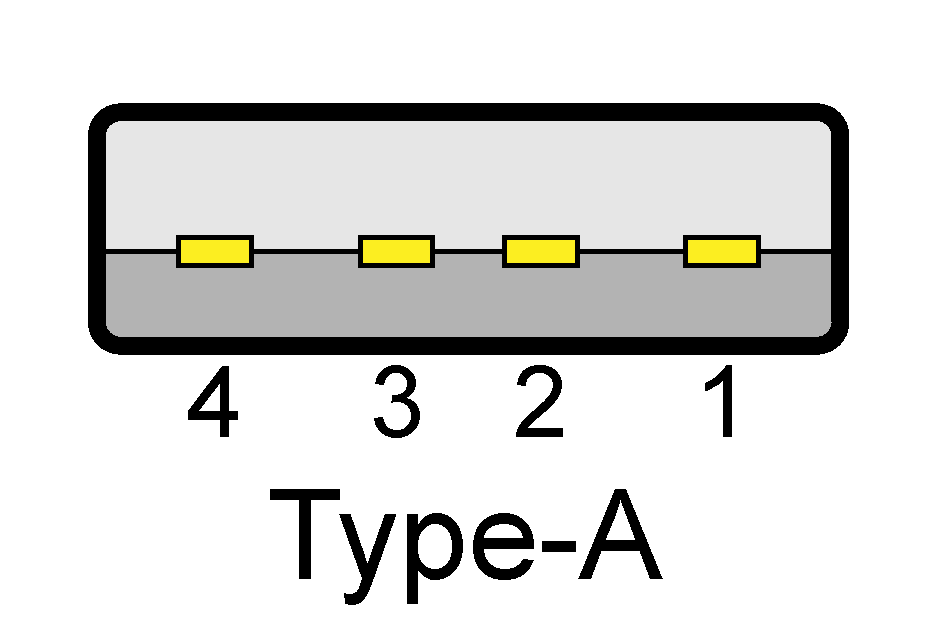
\includegraphics[width=\linewidth]{USB_Type-A.pdf}
    \caption{USB Type-A 公头}
    \label{fig:USB-1}
    \end{subfigure}\hfil % <-- added
    \begin{subfigure}{0.25\textwidth}
    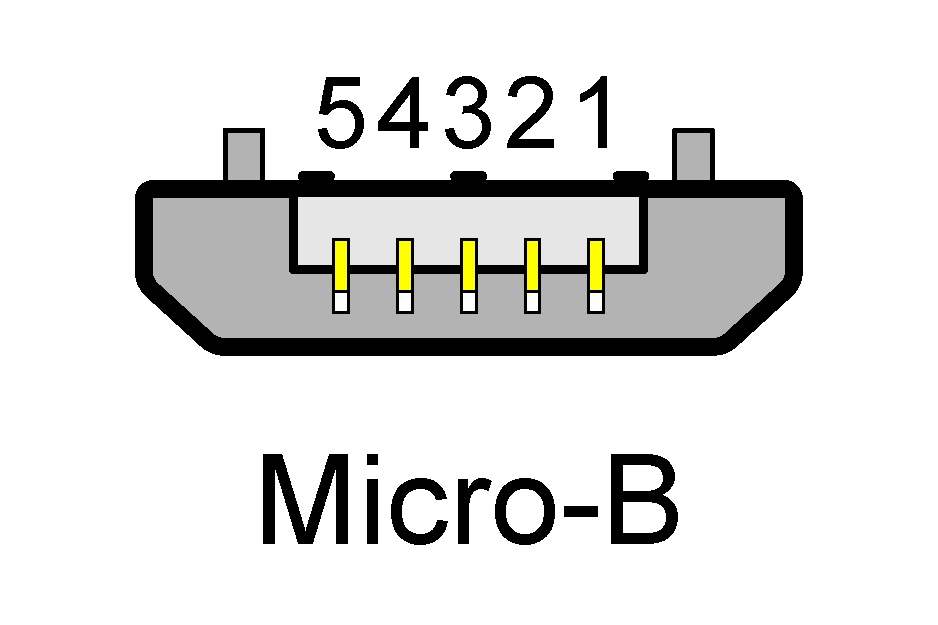
\includegraphics[width=\linewidth]{USB_Micro-B.pdf}
    \caption{USB Micro-B 公头}
    \label{fig:USB-2}
    \end{subfigure}\hfil % <-- added
    \begin{subfigure}{0.25\textwidth}
    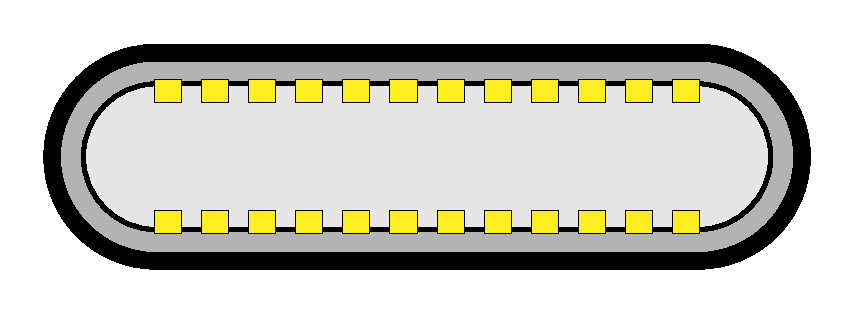
\includegraphics[width=\linewidth]{USB_Type-C_icon.pdf}
    \caption{USB Type-C 公头}
    \label{fig:USB-3}
    \end{subfigure}

    \medskip
    \begin{subfigure}{0.25\textwidth}
    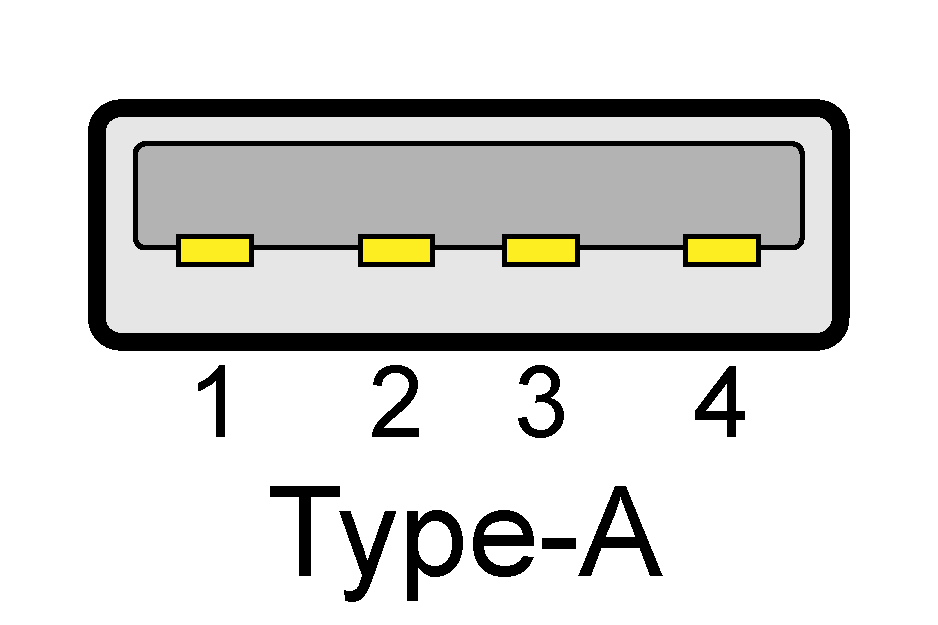
\includegraphics[width=\linewidth]{USB_Type-A_receptacle.pdf}
    \caption{USB Type-A 母头}
    \label{fig:USB-4}
    \end{subfigure}\hfil % <-- added
    \begin{subfigure}{0.25\textwidth}
    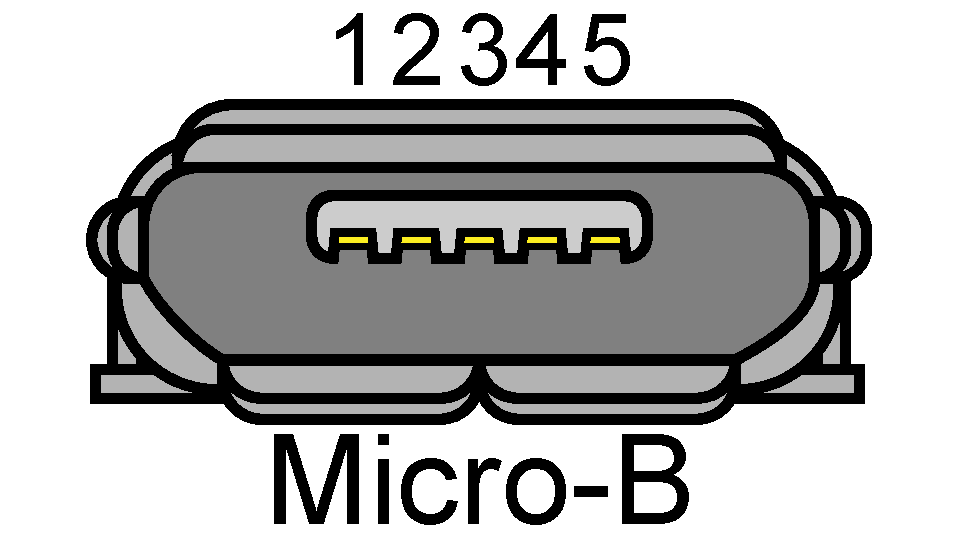
\includegraphics[width=\linewidth]{USB_Micro-B_receptacle.pdf}
    \caption{USB Micro-B 母头}
    \label{fig:USB-5}
    \end{subfigure}\hfil % <-- added
    \begin{subfigure}{0.25\textwidth}
    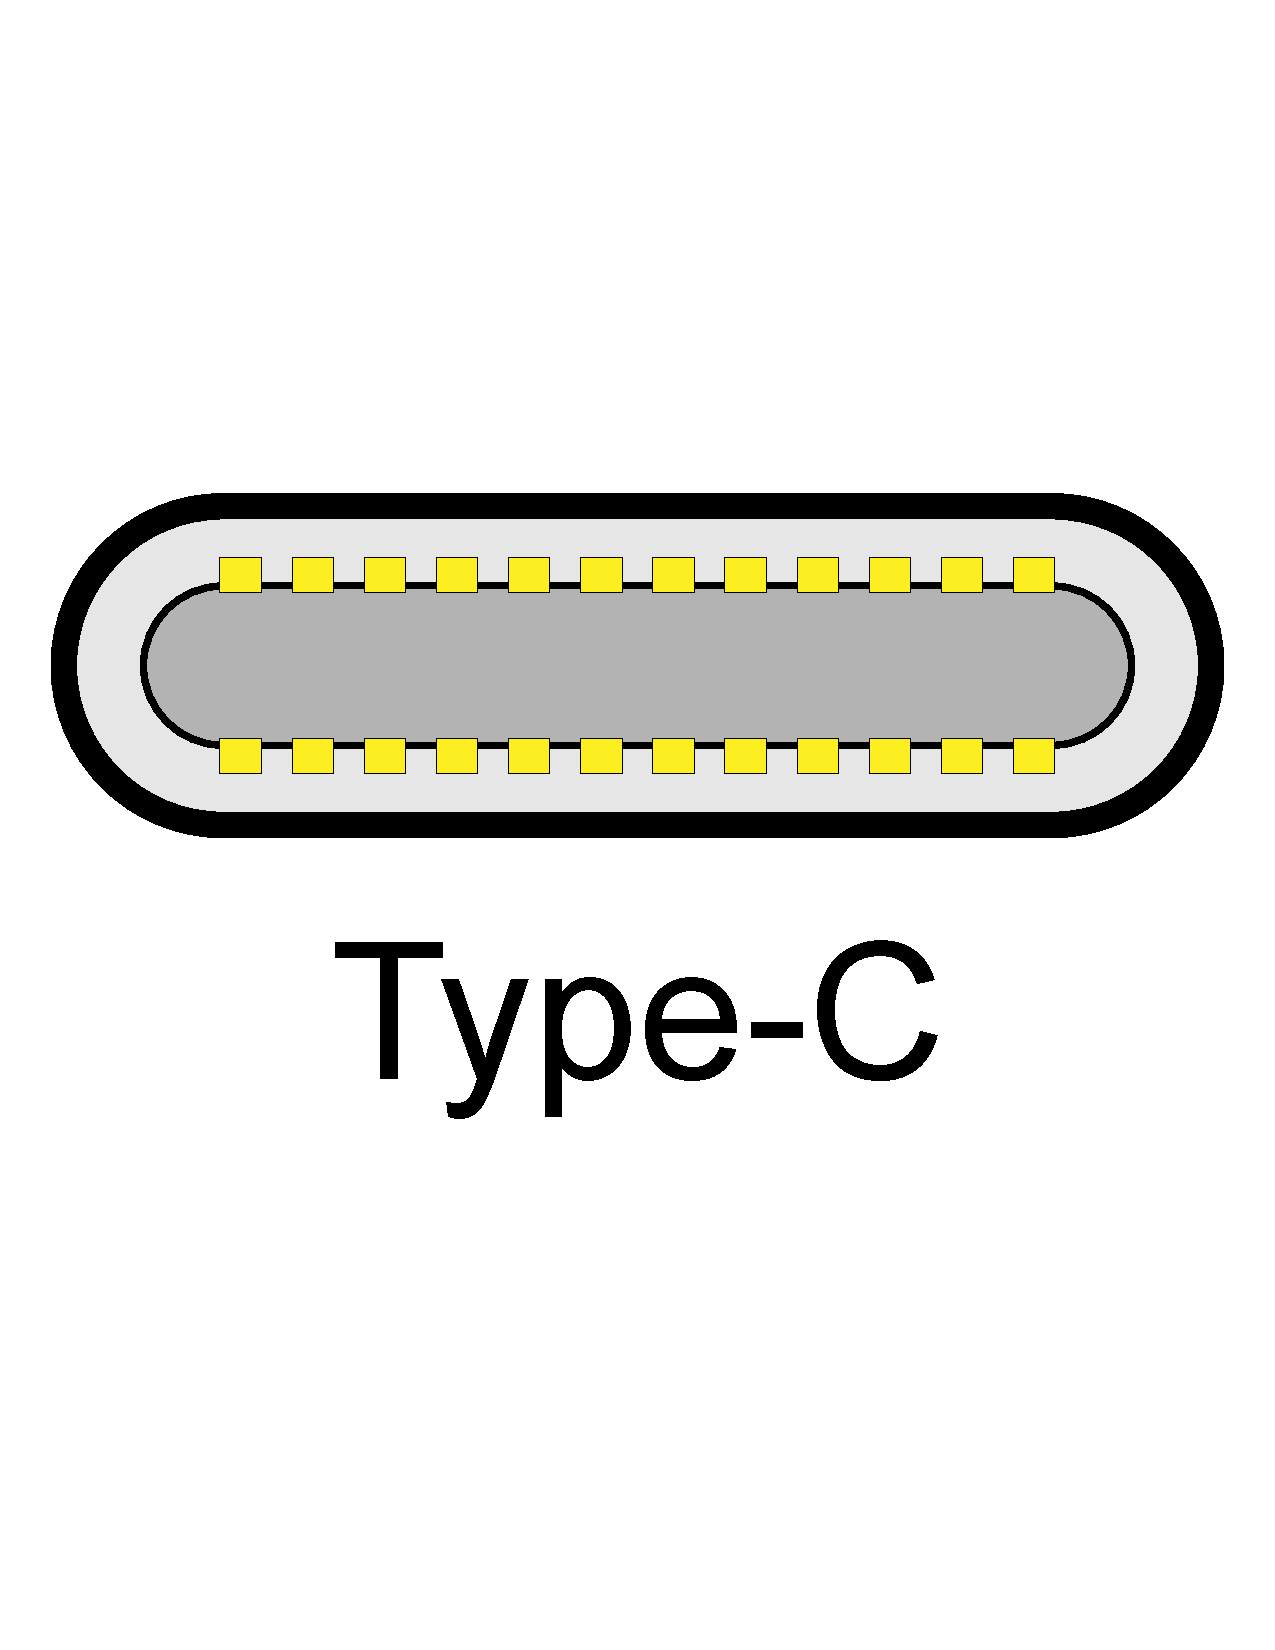
\includegraphics[width=\linewidth]{USB_Type-C_receptacle.pdf}
    \caption{USB Type-C 母头}
    \label{fig:USB-6}
    \end{subfigure}
    \caption{USB 2.0 机械电子标准一览}
    \label{fig:USB-M}
\end{figure}


如表~\ref{fig:USB-M},USB的连接器分为A、B两种,分别用于主机和设备;其各自的小型化的连接器是Mini-A, Mini-B 和 Micro-A, Micro-B,另外还有Mini-AB(可支持Mini-A及Mini-B)的插口。USB 3.1版本中引入了支持正反面不区分插入的C型。

普通电脑上使用的是Type-A口,所以连接电路板时会使用Type-A转Micro USB或Type-C的USB2.0数据线。USB插槽本身还能提供5V的主动电压,及0.5A的电流。

在标准USB接口Type-A中,有四个连接器触点如表~\ref{tab:USB-4},USB信号使用分别标记为D+和D-的双绞线传输,它们各自使用半双工的差分信号并协同工作,以抵消长导线的电磁干扰。

% Please add the following required packages to your document preamble:
% \usepackage{booktabs}
\begin{table}[htbp]
    \centering
    \begin{tabular}{@{}lll@{}}
    \toprule
    触点 & 功能(主机)             & 功能(设备)            \\ \midrule
    1  & V BUS(4.75-5.25 V) & V BUS(4.4-5.25 V) \\
    2  & D-                 & D-                \\
    3  & D+                 & D+                \\
    4  & 接地                 & 接地                \\ \bottomrule
    \end{tabular}
    \caption{标准USB Type-A连接器触点}
    \label{tab:USB-4}
\end{table}

使用Micro-USB机械电子标准的USB插座(母头),此标准常用于移动电话、平板电脑等。Micro-USB将成为移动设备数据和电源的标准接口。

Micro-USB除了第4针外,其他接口功能皆与标准USB相同如表~\ref{tab:MicroUSB}。第4针成为ID,地线在Micro-USB上连接到第5针,在Micro-USB可以悬空亦可连接到第5针。

% Please add the following required packages to your document preamble:
% \usepackage{booktabs}
\begin{table}[htbp]
    \centering
    \begin{tabular}{@{}lll@{}}
    \toprule
    触点 & 功能                & 颜色 \\ \midrule
    1  & V BUS(4.4–5.25 V) & 红  \\
    2  & D−                & 白  \\
    3  & D+                & 绿  \\
    4  & ID                &    \\
    5  & 接地                & 黑 \\ \bottomrule
    \end{tabular}
    \caption{Micro USB连接器触点}
    \label{tab:MicroUSB}
\end{table}

也可以使用支持正反插的USB Type-C接口进行供电和烧写程序,USB Type-C接口常用于新式计算机、移动电话、平板电脑等。其通讯协议和标准见图~\ref{fig:USB-Type-C-pins}和图~\ref{fig:USB-TypeC}。

\begin{figure}[htbp]
    \centering
    \includegraphics[width=\columnwidth]{Figure-2-USB-Type-C-pins.jpg}
    \caption{USB-Type-C-pins}
    \label{fig:USB-Type-C-pins}
\end{figure}

\begin{figure}[htbp]
    \centering
    \includegraphics[width=\columnwidth]{USB-2-To-Type-C.pdf}
    \caption{USB-TypeC}
    \label{fig:USB-TypeC}
\end{figure}



\begin{figure}[htbp]
    \centering
    \includegraphics[]{Mega2560-USB.pdf}
    \caption{Mega2560-USB}
    \label{fig:Mega2560-USB}
\end{figure}

如图~\ref{fig:Mega2560-USB}:

BLM21PG300SN1D为(电感式)片式铁氧体磁珠,阻抗30Ω频率100MHz。

0603ESDA-05N为ESD抑制器/TVS二极管,箝位电压	50V,反向关断电压(典型值)	5V

USB口外壳和内部引线之间并联了ESD二极管和铁氧体磁珠,用于防USB浪涌电流,保护电路。

SMD1812P050TF为PTC自恢复保险丝,最大电压15V,保持电流500mA,最大电流100A,跳闸电流1A,为了防止USB输入电流持续过大。

USB 3.1 C TYPE DIP+SMT CONN为USB Type-C 母头,按照USB2.0协议使用,后续可添加PD或高速数据传输等功能。

\section{RGBLED}

WS2812B是一个集控制电路与发光电路于一体的智能外控LED光源。其外型与一个5050LED灯珠相同,每个元件即为一个像素点。像素点内部包含了智能数字接口数据锁存信号整形放大驱动电路,还包含有高精度的内部振荡器和12V高压可编程定电流控制部分,有效保证了像素点光的颜色高度一致。

数据协议采用单线归零码的通讯方式,像素点在上电复位以后,DIN端接受从控制器传输过来的数据,首先送过来的24bit数据被第一个像素点提取后,送到像素点内部的数据锁存器,剩余的数据经过内部整形处理电路整形放大后通过DO端口开始转发输出给下一个级联的像素点,每经过一个像素点的传输,信号减少24bit。像素点采用自动整形转发技术,使得该像素点的级联个数不受信号传送的限制,仅仅受限信号传输速度要求。

LED具有低电压驱动,环保节能,亮度高,散射角度大,一致性好,超低功率,超长寿命等优点。将控制电路集成于LED上面,电路变得更加简单,体积小,安装更加简便。


\section{ESP32通信模块}

经过BLE4.2和ESP8266的原理性验证,选择ESP32作为通信模块和第二MCU使用。

Espressif ESP32 WROOM 系列\footnote{https://www.espressif.com/zh-hans/products/hardware/esp-wroom-32/overview},基于乐鑫先进的 SoC,ESP32 WROOM 系列模组具备高性能和丰富的外设,集成了 Wi-Fi和蓝牙功能,为先进的物联网应用提供了高度集成的解决方案。

ESP32 WROOM 系列模组包括 ESP32-WROOM-32,ESP32-WROOM-32D 和 ESP32-WROOM-32U 型号,集成了 ESP32 SoC,闪存,精密离散元件和 PCB 板载天线/IPEX 天线,该天线能够在空间有限的应用中提供出色射频性能。

ESP32 WROOM 系列模组具备优化的引脚布局,外设 IO 管脚被分组并引出,将外部走线降低,便于 PCB 板设计,从而使应用更加紧凑。

在本设计中,我们可以灵活选择使用ESP32-WROOM-32/32D/32DC模组,它们的封装和绝大多数功能完全一样。

\begin{figure}[htbp]
    \centering
    \includegraphics[width=\columnwidth]{esp32-wroom-32_datasheet_cn_Outside.pdf}
    \caption{ESP32-WROOM-32 外围原理图}
    \label{fig:ESP32Outside}
\end{figure}

如图~\ref{fig:ESP32Outside}:

注意:

\begin{itemize}
    \item MTDI 应保持低电平。
    \item ESP32-WROOM-32 管脚39,可以不焊接到底板。若将该管脚焊接到底板,确保使用适量的焊锡膏。
    \item 为确保芯片上电时的供电正常,EN管脚处需要增加RC延迟电路。RC通常建议为R = 10kOhms,C = 0.1uF,但具体数值仍需根据模组电源的上电时序和芯片的上电复位时序进行调整。
\end{itemize}

\begin{figure}[htbp]
    \centering
    \includegraphics[]{esp32-wroom-32_datasheet_cn_Reset.pdf}
    \caption{ESP32-WROOM-32复位电路}
    \label{fig:ESP32Reset}
\end{figure}

如图~\ref{fig:ESP32Reset},当使用电池给ESP32系列芯片和模组供电时,为避免电池电压过低导致芯片进入异常状态不能正常启动,一般推荐外接Power Supply Supervisor。建议检测到供给ESP32的电压低于2.3V 时将ESP32的CHIP PU脚拉低。

% \begin{figure}
%     \begin{minipage}{0.48\textwidth}
%       \centering
%       \includegraphics[width=\columnwidth]{ESP32-DevKitC-functional-overview.jpg}
%       \caption{ESP32-DevKitC实物图}
%       \label{fig:ESP32-1}
%     \end{minipage}\hfill
%     \begin{minipage}{0.48\textwidth}
%       \centering
%       \includegraphics[width=\columnwidth]{ESP32-DevKitC-32D.png}
%       \caption{ESP32-DevKitC模型图}
%       \label{fig:ESP32-2}
%     \end{minipage}
% \end{figure}

\begin{figure}[htbp]
    \centering
    \includegraphics[width=\columnwidth]{ESP32-DevKitC-functional-overview.jpg}
    \caption{ESP32-DevKitC实物图}
    \label{fig:ESP32-1}
\end{figure}


\begin{figure}[htbp]
    \centering
    \includegraphics[width=0.48\textwidth]{ESP32-DevKitC-32D.png}
    \caption{ESP32-DevKitC模型图}
    \label{fig:ESP32-2}
\end{figure}

ESP32周边程序烧写设计参考ESP32-DevKitC V4\footnote{\url{https://docs.espressif.com/projects/esp-idf/zh_CN/latest/hw-reference/get-started-devkitc.html}}。如图~\ref{fig:ESP32-1},ESP32-DevKitC 是一款入门级开发板。板上集成的 ESP32 引脚均已引出,便于连接和使用。

管脚 D0、D1、D2、D3、CMD 和 CLK 用于 ESP32 芯片与 SPI flash 间的内部通信,集中分布在开发板两侧靠近 USB 端口的位置。通常而言,这些管脚最好不连,否则可能影响 SPI flash / SPI RAM 的工作。

管脚 GPIO16 和 GPIO17 仅适用于板载 ESP32-WROOM 系列和 ESP32-SOLO-1 的开发板,保留内部使用。

可以直接通过JTAG给ESP32烧写程序,可以通过UART烧写。

1x4的JTAG Header用于软件调试JTAG,直接连接至模块相应引脚上。EN管脚处增加了Datasheet建议的RC延迟电路,并增加了手动控制IO0和EN的轻触开关。

CP2102N-A01-GQFN20R作为USB-UART芯片,不使用其内置3.3V电压转换模块(即供电类型定义为自驱动而非USB总线驱动),通过此芯片可以直接通过USB给ESP32烧写程序。优点是廉价,缺点则为CP2102N只能烧写程序,而不能作为 USB-to-JTAG 接口进行ESP32和计算机的实时通信桥梁。

\begin{figure}[htbp]
    \centering
    \includegraphics[]{CP2104-F03-GMR_System.pdf}
    \caption{CP2104-F03-GMR系统示例图}
    \label{fig:CP2104-F03-GMR}
\end{figure}

后更新为QFN-24-4x4x05P封装的CP2104-F03-GMR芯片,如图~\ref{fig:CP2104-F03-GMR},这一版本的设计参考了官方Datasheet和Github开源项目ESP-Debugger\footnote{\url{https://github.com/xiongyumail/ESP-Debugger}}中的部分电路。

\begin{figure}[htbp]
    \centering
    \includegraphics[]{CP2104-F03-GMR-Regulator-Bypass.pdf}
    \caption{CP2104不使用电平转换示例图}
    \label{fig:CP2104-Regulator-Bypass}
\end{figure}

如图~\ref{fig:CP2104-Regulator-Bypass},在本项目中,VIO和VDD连在一起并通过4.7kOhm的电阻和RST连在一起,REGIN也和VIO VDD连起来,靠近这三个引脚的地方有1uF和100nF的接地电容滤波。另外,接入芯片VBUS的是USB输入的5V经过电阻分压得到的接近3.3V的电压。

SRV05-4HTG为TVS二极管,用于防止过电压对电路的冲击,可以将电压钳位在0-5V之间。在USB口输入的时候用了一个SRV05-4来防止USB输入的静电冲击,在CP2104和ESP32之间用一个SRV05-4防止CP2104可能的工作异常导致ESP32的损坏,经过查阅ESP32的Datasheet发现,ESP32工作电压/供电电压为3.0-3.6V,而非5V,所以这里将电压钳位在0-3.3V之间,并设置一个2x3 UART口作为引出测试用。

NPN三极管S8050用作 DTR RTS --\textgreater EN IO0 逻辑转换,于用驱动EN IO0自动烧写程序,其逻辑真值表见表~\ref{tab:LogicTab}

% Please add the following required packages to your document preamble:
% \usepackage{booktabs}
\begin{table}[htbp]
    \centering
    \begin{tabular}{@{}llll@{}}
    \toprule
    DTR & RTS & EN & IO0 \\ \midrule
    1   & 1   & 1  & 1   \\
    0   & 0   & 1  & 1   \\
    1   & 0   & 0  & 1   \\
    0   & 1   & 1  & 0   \\ \bottomrule
    \end{tabular}
    \caption{DTR RTS --\textgreater EN IO0 逻辑真值表}
    \label{tab:LogicTab}
\end{table}

% 无法Resize的PNG
% \begin{figure}[htbp]
%     \centering
%     \includegraphics[]{esp-wrover-kit-v4.1-layout-front.png}
%     \caption{ESP WROVER KIT实物图}
%     \label{fig:ESP32-WROVER-0}
% \end{figure}

\begin{figure}[htbp]
    \centering
    \includegraphics[width=0.7\columnwidth]{esp-wrover-kit-vb.png}
    \caption{ESP WROVER KIT模型图}
    \label{fig:ESP32-WROVER}
\end{figure}

参考ESP WROVER KIT(如图~\ref{fig:ESP32-WROVER})设计。ESP-WROVER-KIT-VB 为乐鑫 ESP-WROVER-KIT 开发板的变体,默认贴片 ESP32-WROVER-B 模组,支持 LCD 和 MircoSD 卡。板上 ESP32-WROVER-B 模组的 I/O 管脚均已引出,允许用户连接丰富的外设,满足多种开发场景。此外,本款开发板还载有支持多种协议的 USB 转接桥 (FTDI FT2232HL),允许用户直接通过 USB 接口使用 JTAG 调试 ESP32 模组,极大地降低了二次开发的复杂度和成本。

FT2232 多协议 USB 转串口桥接器。开发人员可通过 USB 接口对 FT2232 芯片进行控制和编程,与 ESP32 建立连接。FT2232 芯片可在通道 A 提供 USB-to-JTAG 接口功能,并在通道 B 提供 USB-to-Serial 接口功能,便利开发人员的应用开发与调试。详见 ESP-WROVER-KIT V4.1 原理图。

在更成熟版本的开发中,还可以让FT2232的A路输出到Mega2560,B路输出到ESP32,实现一个芯片和USB口对两个芯片编程。

ESP32可以创建3个UART通信端口,其中UART0被烧写占用,UART1和2均可作为和Arduino通信的接口

注意,ESP32-WROOM-32引脚对应图中GPIO和IO的编号不是对应的!

ESP32-WROOM-32的17号引脚SHD/SD2*可以作为U1RXD,18号引脚SWP/SD3*可以作为U1TXD,将他们分别连接到MEGA2560的TX2(PH1 Digital pin 16)和RX2(PH0 Digital pin 17)引脚上。


\section{电机驱动}

TB6612FNG\footnote{之前使用的TB6612芯片近期国内断货,所以改用A4950、L293D等替代,但是没找到封装。}是双H桥直流电机驱动器,该模块相对于传统的L298N效率上提高很多,体积上也大幅度减少。TB6612FNG每通道输出最高1.2 A的连续驱动电流,启动峰值电流达2A/3.2 A(连续脉冲/单脉冲),4种电机控制模式:正转/反转/制动/停止,PWM支持频率高达100 kHz。

H桥驱动如图~\ref{fig:TB6612FNG-H}所示,可以控制电机正反转,t2和t4为防止短路的死区时间。

\begin{figure}[htbp]
    \centering
    \includegraphics[height=8cm]{TB6612FNG-H.pdf}
    \caption{H桥原理图}
    \label{fig:TB6612FNG-H}
\end{figure}

TB6612FNG的布线按照Datasheet的推荐布线(如图~\ref{fig:TB6612FNG-Connection})设置。

\begin{figure}[htbp]
    \centering
    \includegraphics[width=\columnwidth]{TB6612FNG-Connection.pdf}
    \caption{TB6612FNG典型应用接线图}
    \label{fig:TB6612FNG-Connection}
\end{figure}

步进电机驱动可以采用L6226QTR。

如果未来搭建更大的平台,使用10A级别的电机可以使用ST powerSTEP01 (System-in-package integrating microstepping controller and
10 A power MOSFETs) 作为2相步进电机驱动,在Altium Designer 20环境下也有相应的封装可用,目前平台较小,没有必要使用powerSTEP01。

ST powerSTEP01可以放在额外的驱动板上,作为扩展板使用。ST powerSTEP01支持SPI串行通信,可以只通过一个SPI Bus总线控制多个电机,以菊花链(Daisy chain,如图\ref{fig:SPI_three_slaves_daisy_chained})的形式。注意,ST powerSTEP01供电电压是7.5 V - 85 V,所以2S锂电的7.4V不足以供电,须使用3S及以上锂电池驱动系统,或另加升压模块(不建议)。

\begin{figure}[htbp]
    \centering
    \includegraphics[]{SPI_three_slaves_daisy_chained.pdf}
    \caption{SPI 菊花链(Daisy chain)}
    \label{fig:SPI_three_slaves_daisy_chained}
\end{figure}

串行外设接口(Serial Peripheral Interface Bus,SPI),是一种用于芯片通信的同步串行通信接口规范,主要应用于单片机系统中。SPI设备之间使用全双工模式通信,是一个主机和一个或多个从机的主从模式。主机产生待读或待写的帧数据,多个从机通过一个片选线路决定哪个来响应主机的请求。

SPI总线规定了4个保留逻辑信号接口:

\begin{itemize}
    \item SCLK/SCK(Serial Clock):串列时脉,由主机发出
    \item MOSI(Master Output,Slave Input):主机输出从机输入信号,由主机发出
    \item MISO(Master Input,Slave Output):主机输入从机输出信号,由从机发出
    \item SS/CS(Slave Selected):选择信号,由主机发出,一般是低电位有效
\end{itemize}

在低速时,电压模式控制更有利,而在高速时,或者马达必须经过共振阶段,电流模式是更适合。所以布线参考ST powerSTEP01 Typical application schematic - voltage mode中的走线,如图~\ref{fig:powerstep01}。

\begin{figure}[htbp]
    \centering
    \includegraphics[width=\columnwidth]{powerstep01.pdf}
    \caption{ST powerSTEP01 Typical application schematic}
    \label{fig:powerstep01}
\end{figure}

\section{电机接口}

使用JST端子(\url{https://en.wikipedia.org/wiki/JST_connector})作为电机线缆连接器。

每个代号都是一个系列的产品,他们最大的区别就是Pitch(间距)不一样。

驰海电机GM12-10BY 微型步进减速电机 2相4线 电机与轴同向倒装结构 DC5V ,需要定制改变引线方向,现在默认的引线会蹭到轮子。其JST端子为ZH-1.25mm端子。

GW12-N20VA永磁蜗轮蜗杆齿轮减速电机(有蜗杆改变90度传动方向),定制加装磁性霍尔编码盘,驱动电压5V,空载转速控制在60rpm。其JST端子为ZH-1.5mm端子。

由于ZH接口不是通用接口,所以在PCB上,我们统一使用JST PH 2.0mm公头SMT贴片端子,灵活选用立式卧式端子座。

\section{电源接口}

很多1S锂电池的接口是JST接口,JST接口防反插且很难拔下来,所以我们直接用JST作为我们的电源接口。

一般1S锂电PH2.0(PH 2.00 mm (0.079 in))插口的一号脚为正极,但是1S锂电额定电压是3.7V,使用场景有限。

选用450mAh 2s 7.4V锂电池,保证了电压大于6V、放电能力强劲、容量足够的同时做到电池体积最小化。\url{https://detail.tmall.com/item.htm?id=579993955200}

2s锂电池的接口是JST SFHR 2Pin母头,需要使用 SM02B-SFHRS-TF(LF)(SN) 针脚座连接。如果没有此针脚座封装,可以自行改成PH2.0。


\section{XBEE}

\begin{figure}[htbp]
    \centering
    \includegraphics[width=0.7\columnwidth]{XB-ecosys-hardware-featured.png}
    \caption{Digi XBee RF Modules}
    \label{fig:XB}
\end{figure}

XBEE模块是可提供与设备的无线端点连接的嵌入式解决方案。(如图~\ref{fig:XB})模块使用IEEE 802.15.4网络协议进行快速的点对点网络或对等网络。专为要求低延迟和可预测通信时序的高吞吐量应用而设计\footnote{\url{https://www.sparkfun.com/pages/xbee_guide}}。

DIGI XBEE 3 MICRO FORM FACTOR (XB3-24Z8CM  Digi XBee 3 PRO ZigBee 3.0, 2.4 GHz, Micro, Chip Ant, MMT) 只有13mm x 19mm,可以直接SMT到PCB上,是本应用场景下体积性能的最优解。

XBEE模块直接通过TX-RX和MCU通信,也可以选择直插式模块XBEE-Pro用排针座连接到本项目主板上。模块选型见\url{https://www.digi.com/xbee}

在Altium Designer 20环境下绘制的PCB选取了37 Pin 21.996x33.782mm Pitch 2.007mm的SMT表贴封装,同时兼容XBEE-3系列如XB3-24Z8PS(Digi XBee 3 PRO, 2.4 Ghz Zigbee 3.0, PCB Ant, SMT)和XBEE-S2C系列模块如XB24CZ7PIS-004(Digi XBee ZigBee SMT, PCB Antenna),可以在PCB上直接更换,如图~\ref{fig:XB24CZ7RIS-004}和图~\ref{fig:xbee3}。

测试时可以使用TH MT即通孔安装的封装,未来进一步小型化、SMT自动化可以使用MMT安装方式的封装即Digi XBee 3 Zigbee 3.0, 2.4 GHz, Micro来进一步减小体积。

\begin{figure}
    \begin{minipage}{0.48\textwidth}
      \centering
      \includegraphics[height=6cm]{xbee-zigbee-smt-XB24CZ7RIS-004.jpg}
      \caption{Digi XBee ZigBee SMT}
      \label{fig:XB24CZ7RIS-004}
    \end{minipage}\hfill
    \begin{minipage}{0.48\textwidth}
      \centering
      \includegraphics[height=6cm]{digi-xbee3-smt-pcb-hero.jpg}
      \caption{Digi XBee3, PCB Ant, SMT}
      \label{fig:xbee3}
    \end{minipage}
\end{figure}

为了XBee模块能和Mega2560串口通信,XBee模块的DIN/CONFIG/DIO14连接Mega2560的PD3 ( TXD1/INT3 ) Digital pin 18 (TX1)接口,DOUT/DIO13连接Mega2560的PD2 ( RXDI/INT2 ) Digital pin 19 (RX1)接口。

\section{扩展接口}

三明治扩展形式,层层堆叠,注意厚度。

\section{定位模块}

定位模块采用SONiX OID SNM9S500C3000A Decoder SoC Module,结合桌面上的特殊纸张进行定位。

需要结合EEPROM和校准器使用,所以预留了一个1x7Pin的引脚用于校准。

\begin{figure}[htbp]
    \centering
    \includegraphics[width=\columnwidth]{SONIX_OID_SNM9S500C3000A_Specification_V1.jpg}
    \caption{定位模块Datasheet}
    \label{fig:Camera}
\end{figure}

将摄像头模块的2WIRE-SCK接到Mega2560的PD0 ( SCL/INT0 ) Digital pin 21 (SCL),2WIRE-SDIO接到Mega2560的PD1 ( SDA/INT1 ) Digital pin 20 (SDA)接口,并注意将原Arduino Mega 2560设计中的SDA SCL的5V上拉删去或改成3.3V。

\section{工艺参数}

打样采用嘉立创,工艺参数详见\url{https://www.sz-jlc.com/portal/vtechnology.html}

关键参数如下:双面板过孔最小内径0.3mm,最小外径0.6mm;焊盘边缘到线距离 5mil;单双面板线隙5 mil

以下枚举几个参数的设置,以Minimum-Preferred-Maximum的格式给出:

设置Routing Width为5-10-20mil

Via通孔 孔径0.3-0.4-0.711mm 外径0.6-0.8-1.27mm

Track to Track/SMD Pad/TH Pad Clearance 为 6mil

TH Pad to TH Pad Clearance 为 5mil (Type-C接口要求)

SMD Pads - Fill Clearance -- 0 mil   SMD Pads - Track -- 0 mil     XBEE模块的天线KEEPOUT FILL

SMD Neck-down Rules = 60\%

注意!位号不能有空格,不然JLCSMT会出问题

BOM中不属于JLC基础库的需要每种加20换料费,所有全贴片目前太贵了,所以只贴了核心的芯片和电阻电容,将来批量生产再全面SMT,这一批测试板目前很多元件是手焊的。


\begin{figure}[htbp]
    \centering
    \includegraphics[width=\columnwidth]{JLC-BOM.png}
    \caption{JLC-BOM}
    \label{fig:JLC-BOM}
\end{figure}

\begin{figure}[htbp]
    \centering
    \includegraphics[width=\columnwidth]{JLC-SMT-SIMU.png}
    \caption{JLC-SMT-SIMU}
    \label{fig:JLC-SMT-SIMU}
\end{figure}

\begin{figure}[htbp]
    \centering
    \includegraphics[width=0.8\columnwidth]{Manufacture-v1-1.png}
    \caption{Manufacture-v1}
    \label{fig:Manufacture-v1-1}
\end{figure}

\begin{figure}[htbp]
    \centering
    \includegraphics[width=0.8\columnwidth]{Manufacture-v1-2.png}
    \caption{Manufacture-v1-2}
    \label{fig:Manufacture-v1-2}
\end{figure}

Test Board 3D仿真如图~\ref{fig:TestBoard3D}和图~\ref{fig:TestBoard3D-2}

\begin{figure}[htbp]
    \centering
    \includegraphics[width=\columnwidth]{TestBoard3D.png}
    \caption{Test Board 3D仿真}
    \label{fig:TestBoard3D}
\end{figure}

\begin{figure}[htbp]
    \centering
    \includegraphics[width=0.8\columnwidth]{TestBoard3D-2.png}
    \caption{Test Board 纵向3D仿真}
    \label{fig:TestBoard3D-2}
\end{figure}

\section{实物图}

Test Board 实物图如图~\ref{fig:TestBoard}和图~\ref{fig:TestBoard-SMT}。

\begin{figure}[htbp]
    \centering
    \includegraphics[width=\columnwidth]{TestBoard.jpg}
    \caption{Test Board 实物图}
    \label{fig:TestBoard}
\end{figure}

\begin{figure}[htbp]
    \centering
    \includegraphics[width=0.8\columnwidth]{TestBoard-SMT.jpg}
    \caption{SMT贴片后的Test Board}
    \label{fig:TestBoard-SMT}
\end{figure}

\section{总结}

在第一个版本的测试PCB中,由于疫情的影响,PCB代工厂产能受限,在不明确交期的情况下,只能尽量做到应有尽有。

Mega2560主MCU,做简单的数据处理和电机/通信控制;ATMega16U2可以通过USB Type C口烧写程序;步进电机和直流减速电机驱动;9 x WS2812B RGB-LED全彩灯光显示;下视红外摄像头配合点点纸做定位;XBee3做主要的Mesh组网通信;乐鑫的ESP-32做WiFi 5 、蓝牙、BLE备用通信和第二MCU,CP2102可以通过USB Type C口烧写程序;外置电池稳压供电;USB口供电Buck DC-DC和冲激反压过压过流保护;还有一大堆引出的测试用可编程引脚。

在这一版本的TestBoard上,我验证了大部分硬件原理的正确性和可行性,为下一步做正式版本的板子奠定了基础。
\chapter{PCB 2.0 设计和测试}
\label{cha:PCB-v2}

本章设计源文件和历史版本详见\url{https://github.com/TingliangZhang/Misaka-PCB-v2}

\section{需要解决的问题}

在测试版本的PCB(PCB v1)中出现了不少经过测试发现的问题,在第二版本中尽可能予以纠正:

\begin{itemize}
    \item ATmega2560的晶振封装无法手焊,而且不在嘉立创基础库里,不方便SMT
    \item PowerSTEP01过于昂贵,而且极难手动贴片。
\end{itemize}

\section{设计环境的更改}

PCB的设计依赖电子设计自动化(英语:Electronic design automation,缩写:EDA)软件。

当初绘制PCB v1时使用的时Altium Designer 20.0.9集成开发环境。

由于AD20是商业付费EDA软件,而且之前的绘制使用了Altium Live 在线供应商封装库,可移植性和便携性不是很好,即使生成了Integrated Library,也很难找到成套的规范化封装。另外AD20的源文件不是普通编辑器可以打开的文本,这使得Git代码管理变得困难。

基于以上考量,改用KiCAD开源EDA软件进行目前及将来的电路设计,如图~\ref{fig:kicad_flowchart}。

\begin{figure}[htbp]
    \centering
    \includegraphics[width=\columnwidth]{kicad_flowchart.png}
    \caption{KiCad Workflow}
    \label{fig:kicad_flowchart}
\end{figure}

\section{MCU}

参考了Mega Pro Embed CH340G / ATmega2560 board \footnote{\url{https://robotdyn.com/mega-2560-pro-embed-ch340g-atmega2560-16au.html}}的设计,如图~\ref{fig:MEGA-PRO-CH340GATmega2560}。

\begin{figure}[htbp]
    \centering
    \includegraphics[width=\columnwidth]{MEGA-PRO-CH340GATmega2560.jpg}
    \caption{Mega Pro Embed CH340G / ATmega2560}
    \label{fig:MEGA-PRO-CH340GATmega2560}
\end{figure}

\chapter{PCB 3.0 改进设计和测试}
\label{cha:PCB-v3}

\section{待改进问题}

三路驱动丝印编号

电池插头+-反向,以丝印标注

芯片周围留出clearance,方便拖焊。摆放可以考虑45度角摆放,方便密集的布线。

最好改成单面有贴片元件的形式,方便SMT或者制作钢网涂锡膏。

选用没有ThermalVias的芯片封装,否则容易焊锡粘到了ThermalVias上引起不平整。(但是没有不含ThermalPad的封装)

留出STEP和DIR测试/备用引脚,以便板上有一两片DRV8825无法正常使用可以外接模块。

12V和5V供电太细了,要注意供电可靠性。

扩大PCB面积,从100mm到120mm直径圆内接正六边形。

Reset按钮封装不对。Reset电路中R22/D1,RESET BUTTON/C13不是必须的,可以画,可以不焊。

!!!发现CH340C的TX接到了Mega的TX上,RX接到了Mega的RX上,所以烧录Arduino时出现错误:

\begin{tcolorbox}
    avrdude: stk500v2\_ReceiveMessage(): timeout \\
    avrdude: stk500v2\_getsync(): timeout communicating with programmer
\end{tcolorbox}


\section{外形}

小车外轮廓为120mm圆内接正六边形,为了尽可能放到单面上,设计成120mm圆内接正六边形,加上40mm半径处3mm直径的M3螺丝定位孔,注意孔位置在边上而不是角上。注意Fusion360导出草图的操作是直接右键草图另存为DXF!

\section{原理图更改}

在这个版本,删去了一些演示中暂时用不到的模块:

\begin{itemize}
    \item RGB-LED阵列
    \item 下视相机模块
    \item 控制步进的拨码开关
    \item Reset按钮和电容/CD1206二极管
\end{itemize}

同时将XT30的正负极反向,修正了封装和实际不对应的问题。

TX0和RX0倒序,纠正了错误。

原理图如图~\ref{fig:MisakaPCBv3-sch}。

\begin{figure}[htbp]
    \centering
    \includegraphics[width=\columnwidth]{MisakaPCBv3-1.pdf}
    \caption{PCBv3原理图}
    \label{fig:MisakaPCBv3-sch}
\end{figure}

\section{PCB绘制}

将MCU倾斜45度,方便布线。

加粗12V和5V干线至1mm宽。

三个电机驱动模块统一布局布线,使其具有相似性,并变得整齐。

考虑到走线问题,同一功能的信号线组并在一起。

布线之后的PCB详见附录~\ref{sec:PCB}。

布线之后的PCB(未显示铺铜)如图~\ref{fig:MisakaPCBv3-1}、~\ref{fig:MisakaPCBv3}。

\begin{figure}[htbp]
    \centering
    \includegraphics[width=\columnwidth]{MisakaPCBv3-2.pdf}
    \caption{PCBv3布线}
    \label{fig:MisakaPCBv3}
\end{figure}

\begin{figure}[htbp]
    \centering
    \includegraphics[width=\columnwidth]{MisakaPCBv3-1.png}
    \caption{PCBv3布线之后的PCB}
    \label{fig:MisakaPCBv3-1}
\end{figure}

\section{三维渲染图}

使用光线追踪技术对PCB模型进行渲染得到正面的渲染图如图~\ref{fig:MisakaPCBv3-2}、~\ref{fig:MisakaPCBv3-3}。

\begin{figure}[htbp]
    \centering
    \includegraphics[width=\columnwidth]{MisakaPCBv3-2.png}
    \caption{正面渲染图}
    \label{fig:MisakaPCBv3-2}
\end{figure}

\begin{figure}[htbp]
    \centering
    \includegraphics[width=\columnwidth]{MisakaPCBv3-3.png}
    \caption{光追渲染图}
    \label{fig:MisakaPCBv3-3}
\end{figure}

\section{其他问题}

应当加一个ON LED作为电源指示灯。

没有Reset很麻烦,特别是一开始调试的时候,需要按Reset重置代码。考虑加一个Reset按钮到GND和一个22pF电容并连。

\chapter{开发环境的配置}
\label{cha:Environment}

在这一章,着重阐述Windows 10环境下开发环境的配置方法。

\section{Mega 2560开发环境}


\section{ESP 32开发环境配置}

\subsection{Windows平台ESP-IDF工具链的标准设置}

ESP-IDF 需要安装一些必备工具,才能围绕 ESP32 构建固件,包括 Python、Git、交叉编译器、menuconfig 工具、CMake和 Ninja 编译工具等。

要安装 ESP-IDF 必备工具,最简易的方式是下载 ESP-IDF 工具安装器\footnote{\url{https://dl.espressif.com/dl/esp-idf-tools-setup-2.2.exe}}。

安装器可安装所需的交叉编译器、OpenOCD、cmake 和 Ninja 编译工具,以及一款 mconf-idf 配置工具。此外,本安装器还可在有需要时下载、运行 Python 3.7 和 Git For Windows 的安装器,如图~\ref{fig:IDF-Installer}。

\begin{figure}[htbp]
    \centering
    \includegraphics[width=0.7\columnwidth]{IDF-Installer.png}
    \caption{ESP-IDF 工具安装器配置}
    \label{fig:IDF-Installer}
\end{figure}

\subsection{获取 ESP-IDF}

除了工具链,您还需要供 ESP32 使用的 API(软件库和源代码),具体请见 ESP-IDF 仓库。

请将 ESP-IDF 下载到您的本地。

获取本地副本:打开终端,切换到你要存放 ESP-IDF 的工作目录,使用 \mintinline{powershell}|git clone| 命令克隆远程仓库:

% \mint{powershell}|git clone -b v4.0-rc --recursive https://github.com/espressif/esp-idf.git|


GitHub 中”下载 zip 文档”的功能不适用于 ESP-IDF,所以需要使用 git clone 命令。作为备份,可以在没有安装 Git 的环境中下载 Stable version 的 zip 归档文件。直接在\url{https://github.com/espressif/esp-idf/releases/download/v4.0-rc/esp-idf-v4.0-rc.zip}下载并解压。

\subsection{安装 Python 软件包}

ESP-IDF 所需的 Python 软件包位于 IDF-PATH/requirements.txt 中。您可以运行以下命令进行安装:

\mint{powershell}|python -m pip install --user -r $IDFPATH/requirements.txt|

\begin{tcolorbox}
    This is my first \textbf{tcolorbox}.
\end{tcolorbox}

\subsection{开始创建工程}

现在,您可以开始准备开发 ESP32 应用程序了。您可以从 ESP-IDF 中 examples 目录下的 get-started/hello-world 工程开始。ESP-IDF 编译系统不支持带有空格的路径,可能需要复制到其他目录下再运行。

\subsection{连接设备}

现在,请将您的 ESP32 开发板连接到 PC,并查看开发板使用的串口。

通常,串口在不同操作系统下显示的名称有所不同:

\begin{itemize}
    \item Windows 操作系统: COM1 等
    \item Linux 操作系统: 以 /dev/tty 开始
    \item MacOS 操作系统: 以 /dev/cu. 开始
\end{itemize}


\subsection{工程配置}
\chapter{程序编写}
\label{cha:Program}

\section{VS Code下Arduino编程环境配置}

VS Code下Arduino编程环境配置\footnote{\url{https://docs.microsoft.com/zh-cn/azure/iot-hub/iot-hub-arduino-iot-devkit-az3166-get-started}}
方法如下:

\begin{enumerate}

    \item
        安装 \href{https://www.arduino.cc/en/Main/Software}{Arduino IDE}。此IDE 提供必要的工具链用于编译和上传 Arduino 代码。
        
        \begin{itemize}
        \item
            \textbf{Windows}:使用 Windows Installer 版本,不要从应用商店安装。
        \item
            \textbf{macOS}:将解压缩的 \textbf{Arduino.app} 拖放到\texttt{/Applications} 文件夹中。
        \item
            \textbf{Ubuntu}:解压缩到某个文件夹中,例如 \texttt{\$HOME/Downloads/arduino-1.8.8}
        \end{itemize}
    \item
         安装\href{https://code.visualstudio.com/}{Visual Studio Code}是一个跨平台源代码编辑器,其中包含功能强大的intellisense、代码完成和调试支持以及可从 marketplace 安装丰富的扩展。
    \item
        启动 VS Code,在扩展市场中找到 \textbf{Arduino} 并安装它。此扩展提供在 Arduino 平台上进行开发的增强体验。
    \item
        为 VS Code 配置 Arduino 设置。
        
        在 Visual Studio Code 中,单击 "\textbf{文件" \textgreater{} 首选项 \textgreater{} 设置}(在 macOS 上,\textbf{代码 \textgreater{} 首选项 \textgreater{} 设置})。 然后单击 "\emph{设置}" 页右上角的 "\textbf{打开设置(JSON)} " 图标。

        根据你的平台添加以下行来配置 Arduino:
    
        \textbf{Windows}:
        \begin{tcolorbox}
            "arduino.path": "C:\textbackslash{}\textbackslash{}Program Files (x86)\textbackslash{}\textbackslash{}Arduino",
        \end{tcolorbox}

        \textbf{macOS}:
    
        \begin{tcolorbox}    
            "arduino.path": "/Applications",
        \end{tcolorbox}

        \textbf{Ubuntu}:
    
        将下面的 \textbf{\{username\}} 占位符替换为你的用户名。
        \begin{tcolorbox}
            "arduino.path": "/home/\{username\}/Downloads/arduino-1.8.8",
        \end{tcolorbox}
    \end{enumerate}



\section{TB6612电机测试程序}

在引脚分配时,我们将两片TB6612连接在Mega2560上。

四个PWM调速信号输出引脚由能输出PWM波的PH 3 4 5 6承担,分别接到PWM A B C D,在Arduino IDE程序中对应 Digital pin 6 7 8 9 (PWM)。

每个电机控制的IN1 IN2 分别由 PA0-PA7 8个引脚承担,对应Digital pin 22 - 29,由于只是使能信号,普通数字引脚即可,不需要特定的PWM引脚。

STBY信号由 PG2 ( ALE ) Digital pin 39统一给出,即所有电机统一使能或待机。

\section{WS2812B测试程序}

由PE5 ( OC3C/INT5 ) Digital pin 3 (PWM) 引脚提供串行通信信号。

需要在Arduino IDE 安装Adafruit NeoPixel库,直接通过Library Manager安装即可,如图~\ref{fig:Adafruit-NeoPixel-Installation}。

\begin{figure}[htbp]
    \centering
    \includegraphics[width=\textwidth]{Adafruit-NeoPixel-Installation.png}
    \caption{通过Library Manager安装Adafruit NeoPixel库}
    \label{fig:Adafruit-NeoPixel-Installation}
\end{figure}

本项目测试程序在原有Adafruit NeoPixel库示例程序strandtest上修改而成,可以让9个RGB LED以各种规律发光以测试功能的完备性。


\section{ESP32}

在Arduino IDE内也可以添加对ESP32 Boards的支持,在Arduino IDE设置里的"Additional Board Manager URLs"中添加\url{https://raw.githubusercontent.com/espressif/arduino-esp32/gh-pages/package_esp32_index.json} 以英文逗号和其他网址分隔,之后在Tools > Board > Boards Manager… 内安装 "ESP32 by Espressif Systems"即可。Arduino core for the ESP32也可以在\url{https://github.com/espressif/arduino-esp32}下载源码自己编译。
\chapter{实物可视化界面UI设计}
\label{cha:UI}

本部分代码详见\url{https://github.com/TingliangZhang/Misaka-Jupyter}。

\section{实物可视化界面}

在通信演示例子中,三个固定的小车代表节点,每条有向边上一个小车代表通信协议传输的数据包。
当任何数据包发送的时候,此有向边上对应的小车就会移动到发送节点的旁边(一定距离内认为两者可以相互通信)接收数据包,并显示在它的屏幕上。之后他将朝着目标节点移动,到达目标通信节点周围一定范围后,将数据包发送给目标节点,目标节点再进行一系列的运算,并将过程显示在其屏幕上。

位于车顶的LED颜色既可以代表不同系列的数据,也可以通过渐变色表达第三个独立的变量。


在动态迭代可视化模式下,工作平面视为一个二维坐标系,每一个小车代表一个机组节点,小车在坐标系中纵轴位置代表各自当前出力,随着迭代进行变化,同时隐性地仿真了通信过程,进行去中心化的自治优化,当节点数(新加入或撤出)或任意节点数据变化系统会重新开始动态迭代。物理场景和算法的映射关系如表~\ref{tab:Real-Unreal}。表现形式不一定是位置,也可能是颜色,坐标系也可能会是三维的。

可以通过小车一开始摆放的位置设定初值,迭代过程中或结束后任意时刻可以手动移动小车来改变任意节点的值以干预算法的执行

% Please add the following required packages to your document preamble:
% \usepackage{booktabs}
\begin{table}[htbp]
    \centering
    \begin{tabular}{@{}ll@{}}
    \toprule
    物理场景          & 算法                   \\ \midrule
    桌面            & 二维坐标系                \\
    前后            & 纵轴——电价指数(可能会经过一系列变换) \\
    左右            & 横轴——节点数(均匀分布)        \\
    小车            & 通信节点(拓扑中的点)          \\
    摆放小车          & 设定初始节点数和各节点初始值       \\
    小车运动          & 电价指数改变               \\
    停止在Y坐标相同的一条线上 & 迭代完成,各节点达成共识         \\
    移除小车          & 断开一个节点               \\
    放入小车          & 新增一个节点后自动重新开始迭代      \\ \bottomrule
    \end{tabular}
    \caption{物理场景和算法的映射关系}
    \label{tab:Real-Unreal}
\end{table}

\section{实物可视化界面DEMO}

初始DEMO UI为用PC通过XBee指定节点ID发送Move距离信息,节点收到后即开始运动相应距离,此过程中需要对Step和实际距离进行标定。首次标定得到两电机相反方向转动1000steps约为前进15cm,此时stepsPerRevolution = 200,即steps * stepsPerRevolution = 1000。如图~\ref{fig:MeasureSteps}

\begin{figure}[htbp]
    \centering
    \includegraphics[width=\columnwidth]{MeasureSteps.jpg}
    \caption{对Step和实际距离进行标定}
    \label{fig:MeasureSteps}
\end{figure}

采用的数据参照~\ref{sec:Illustration}小节中的数据设计,考虑到场地有限(宿舍桌面大小),占用纵轴区间长度3对应45cm的可用桌面,比例0.5cm对应1单位,考虑到精度问题,如表~\ref{tab:UIDemoDesign},只取0,1,2,3,8,9,10,13这几组变化较大的数据,如表~\ref{tab:UIDemoDesignSelection}。

\begin{table}[htbp]
    \centering
    \begin{tabular}{|l|l|l|l|l|l|l|l|l|}
    \hline
    \diagbox{迭代次数}{$Y_{i,j}$}{位移} %添加斜线表头
       & 1  & 2  & 3  & 4   & d1 & d2 & d3  & d4  \\ \hline
    0  & 0  & 0  & 0  & 0   &    &    &     &     \\ \hline
    1  & 30 & 60 & 90 & 0   & 30 & 60 & 90  & 0   \\ \hline
    2  & 45 & 75 & 60 & 0   & 15 & 15 & -30 & 0   \\ \hline
    3  & 60 & 68 & 53 & 0   & 15 & -8 & -8  & 0   \\ \hline
    4  & 64 & 60 & 56 & 0   & 4  & -8 & 4   & 0   \\ \hline
    5  & 62 & 58 & 60 & 0   & -2 & -2 & 4   & 0   \\ \hline
    6  & 60 & 59 & 61 & 0   & -2 & 1  & 1   & 0   \\ \hline
    7  & 60 & 60 & 60 & 0   & 0  & 1  & 0   & 0   \\ \hline
    8  & 60 & 60 & 60 & 120 & 0  & 0  & 0   & 120 \\ \hline
    9  & 60 & 60 & 80 & 90  & 0  & 0  & 20  & -30 \\ \hline
    10 & 60 & 70 & 77 & 75  & 0  & 10 & -3  & -15 \\ \hline
    11 & 65 & 73 & 71 & 73  & 5  & 3  & -6  & -2  \\ \hline
    12 & 69 & 72 & 69 & 73  & 4  & -1 & -1  & 0   \\ \hline
    13 & 71 & 71 & 71 & 71  & 2  & -1 & 2   & -2  \\ \hline
    \end{tabular}
    \caption{节点位移比对}
    \label{tab:UIDemoDesign}
\end{table}

\begin{table}[htbp]
    \centering
    \begin{tabular}{|l|l|l|l|l|l|l|l|l|}
    \hline
    \diagbox{迭代次数}{$Y_{i,j}$}{位移} %添加斜线表头
      & 1  & 2  & 3  & 4   & d1 & d2 & d3  & d4  \\ \hline
    0 & 30 & 30 & 30 & 120 &    &    &     &     \\ \hline
    1 & 30 & 60 & 90 & 120 & 0  & 30 & 60  & 0   \\ \hline
    2 & 45 & 75 & 60 & 120 & 15 & 15 & -30 & 0   \\ \hline
    3 & 60 & 68 & 53 & 120 & 15 & -8 & -8  & 0   \\ \hline
    4 & 60 & 60 & 60 & 120 & 0  & -8 & 8   & 0   \\ \hline
    5 & 60 & 60 & 80 & 90  & 0  & 0  & 20  & -30 \\ \hline
    6 & 60 & 70 & 77 & 75  & 0  & 10 & -3  & -15 \\ \hline
    7 & 71 & 71 & 71 & 71  & 11 & 1  & -6  & -4  \\ \hline
    \end{tabular}
    \caption{节点位移选取}
    \label{tab:UIDemoDesignSelection}
\end{table}

对ForwardUnits进行1/6校准到单位位移,对Delay进行1/16校准到1ms。

但是还有一个因素未纳入考虑,小车移动需要时间。要想让他们同时进行运动,还要计算各小车运动的时间。

我们知道,1step对应放缩后的1ms,ForwardUnits(30) 对应的时间为1s,由此设计开始运动时间间隔为3s。减去相应的移动时间即为两次移动中间应当delay的时间。

此Demo小车端代码详见附录~\ref{sec:MisakaCarV1}。

\section{JupyterLab环境配置}

本节代码详见附录~\ref{sec:JupyterLabUI-Code}。

JupyterLab安装参考TUNA的pypi 镜像使用帮助\footnote{\url{https://mirrors.tuna.tsinghua.edu.cn/help/pypi/}},升级 pip 到最新的版本 (>=10.0.0) 后进行配置:

\begin{tcolorbox}
    pip install pip -U \\
    pip config set global.index-url https://pypi.tuna.tsinghua.edu.cn/simple \\
    pip install jupyterlab
\end{tcolorbox}

在CMD或者Powershell中使用以下命令启动jupyter lab:

\begin{tcolorbox}
    jupyter lab
\end{tcolorbox}

ipywidgets\footnote{\url{https://github.com/jupyter-widgets/ipywidgets}}可以使用pip安装,注意安装前关闭Jupyter Lab再安装!

\begin{tcolorbox}
    pip install ipywidgets \\
    jupyter nbextension enable --py --sys-prefix widgetsnbextension  (can be skipped for notebook version 5.3 and above)
\end{tcolorbox}

cookie cutter\footnote{\url{https://github.com/jupyter-widgets/widget-ts-cookiecutter}}是一个很流行的示例项目,可供参考。

流行的widget库包括bqplot\footnote{\url{https://github.com/bloomberg/bqplot}}、pythreejs\footnote{\url{https://github.com/jovyan/pythreejs}}和ipyleaflet\footnote{\url{https://github.com/ellisonbg/ipyleaflet}}等。

Plotly\footnote{\url{https://plot.ly/python/getting-started/}}是一个ipywidgets,用于构建交互式图表。

可以使用pip安装:

\begin{tcolorbox}
    pip install plotly
\end{tcolorbox}

Dependence的安装:

\begin{tcolorbox}
    pip install jupyterlab "ipywidgets"
\end{tcolorbox}

之后需要Enable Plotly并设置环境变量,执行以下命令:

\begin{minted}[breaklines]{python}
    # Avoid "JavaScript heap out of memory" errors during extension installation
    # (OS X/Linux)
    export NODE_OPTIONS=--max-old-space-size=4096
    # (Windows)
    set NODE_OPTIONS=--max-old-space-size=4096

    # Jupyter widgets extension
    jupyter labextension install @jupyter-widgets/jupyterlab-manager --no-build

    # jupyterlab renderer support
    jupyter labextension install jupyterlab-plotly --no-build

    # FigureWidget support
    jupyter labextension install plotlywidget --no-build

    # Build extensions (must be done to activate extensions since --no-build is used above)
    jupyter lab build

    # Unset NODE_OPTIONS environment variable
    # (OS X/Linux)
    unset NODE_OPTIONS
    # (Windows)
    set NODE_OPTIONS=
\end{minted}

用以下代码来测试Plotly是否正确安装:

\begin{minted}[breaklines]{python}
    import plotly.graph_objects as go
    fig = go.Figure(data=go.Bar(y=[2, 3, 1]))
    fig.show()
\end{minted}

\section{演示系统UI}

UI基于Jupyter Lab编写网页端的实时可视化界面。

以下代码的作用是产生一个可通过拖动滑块来交互的直方图界面:

\begin{minted}[breaklines,linenos,python3]{python}
    import plotly.graph_objects as go
    from __future__ import print_function
    from ipywidgets import interact, interactive, fixed, interact_manual
    import ipywidgets as widgets
    from ipywidgets import Button, Layout

    def f(a,b,c,d):
        fig = go.Figure(data=go.Bar(y=[a, b, c, d]))
        fig.show()
        global Input
        Input = [0,0,0,0]
        Input[0]=a
        Input[1]=b
        Input[2]=c
        Input[3]=d
        for i in range(0,4):
            print(Input[i])
        # 在这插入XBee代码
        XbeeTx(Input)
        
    def XbeeTx(Input):
        for i in range(0,4):
            print(Input[i])    

    def XbeeTxRun(RUNorNOT):
        print('Running')           
            
            
    I = [0,0,0,0]

    for i in range(0,4):
        I[i] = widgets.FloatSlider(min=0, max=1e3, step=1)

    ui = widgets.VBox([I[0], I[1], I[2], I[3] ])
    # ui = widgets.HBox([I[0], I[1], I[2], I[3] ])

    out = widgets.interactive_output(f, {'a': I[0], 'b': I[1], 'c': I[2], 'd': I[3] } )

    b1 = Button(description='Run')
    b1.style.button_color = 'lightgreen'
    b1.on_click (XbeeTxRun)


    display(ui, out, b1)
\end{minted}

运行效果如图~\ref{fig:Plotly-0}

\begin{figure}[htbp]
    \centering
    \includegraphics[width=\columnwidth]{Plotly-0.png}
    \caption{Plotly界面交互效果-初始}
    \label{fig:Plotly-0}
\end{figure}

拖动滑块将改变widgets.FloatSlider函数内形参的量,并在函数f中将I这一FloatSlider型变量传递到全局变量Input上(浮点型),显示在下方,效果如图~\ref{fig:Plotly}

\begin{figure}[htbp]
    \centering
    \includegraphics[width=\columnwidth]{Plotly.png}
    \caption{Plotly界面交互效果-拖动}
    \label{fig:Plotly}
\end{figure}

点击Run后,显示的变为小车的实时位置(Y轴),移动平台开始运动,函数开始迭代,逐渐收敛。运行效果如图~\ref{fig:Plotly-1}

\begin{figure}[htbp]
    \centering
    \includegraphics[width=\columnwidth]{Plotly-1.png}
    \caption{Plotly界面交互效果-点击Run后}
    \label{fig:Plotly-1}
\end{figure}

为了演示效果,两次迭代之间加入了1s的延迟。
\chapter{通信协议}
\label{cha:Communication}

\section{RS-232}

RS-232, Recommended Standard 232 \footnote{RS-232, when compared to later interfaces such as RS-422, RS-485 and Ethernet, has lower transmission speed, short maximum cable length, large voltage swing, large standard connectors, no multipoint capability and limited multidrop capability. In modern personal computers, USB has displaced RS-232 from most of its peripheral interface roles.} 是一种串行通信协议。见\url{https://en.wikipedia.org/wiki/RS-232}

我们的Arduino编程器的通信协议就是RS-232。

\section{UART}

通用异步收发传输器(Universal Asynchronous Receiver/Transmitter,通常称为UART)是一种异步收发传输器,是电脑硬件的一部分,将数据透过串列通讯和平行通讯间作传输转换。UART通常用在与其他通讯接口(如EIA RS-232)的连接上。\footnote{\url{https://en.wikipedia.org/wiki/Universal_asynchronous_receiver-transmitter}}

具体实物表现为独立的模组化芯片,或是微处理器中的内部周边装置(peripheral)。一般和RS-232C规格的,类似Maxim的MAX232之类的标准信号幅度变换芯片进行搭配,作为连接外部设备的接口。在UART上追加同步方式的序列信号变换电路的产品,被称为USART(Universal Synchronous Asynchronous Receiver Transmitter)。
\chapter{XBee}
\label{cha:XBee}

\section{AT设置}



\section{固件升级}

本地设备设置AP=2 即 API mode 能使用Network Working Mode,以便升级固件。

用XBee 3 无线连接淘宝买的XBee Pro S2B需要先下载lagacy XBee Firmware。但不能直接无线更新固件,还是需要用USB连接到电脑上烧写新固件。XBee3则可以直接无线更新。

这就决定了小车上尽可能使用XBee3,虽然要比XBee S2B贵3-4倍。当然也可以直接在我们的PCB上画FT232接USB口以便更新固件使用,或者预留编程口直接使用编程线。

只有以下这些模块才能无线更新固件:

\begin{itemize}
    \item XBee/XBee PRO SX
    \item XLR Pro Module
    \item XBee/XBee PRO 802.15.4 (S2C module versions only)
    \item XBee/XBee-PRO DigiMesh 2.4 (S2C module versions only)
    \item XTend RF Module Family (SX module versions only)
    \item XBee/XBee-PRO ZB and Programmable XBee-PRO ZB
    \item XBee/XBee-PRO ZB SMT and Programmable XBee-PRO ZB SMT
    \item XBee-PRO 900HP and Programmable XBee-PRO 900HP
    \item XBee 865LP and Programmable XBee 865LP
    \item XBee3 (Zigbee, DigiMesh 2.4, and 802.15.4)
\end{itemize}


\chapter{3D打印建模}
\label{cha:Model}

\section{Model v1}

测试用3轮底盘需要考虑到电机和定位模块的配合。

定位模块外形为 $\phi$ 11.2 X 25.1mm,至少需要留12mm直径的圆柱形空间,头部距离地面不得超过2mm。定位模块外形尺寸如图~\ref{fig:Camera-Dimension}。

\begin{figure}[htbp]
    \centering
    \includegraphics[width=\columnwidth]{SONIX_OID_SNM9S500C3000A_Specification_V1-Dimension.jpg}
    \caption{定位模块外形尺寸}
    \label{fig:Camera-Dimension}
\end{figure}

定位模块配套母排离PCB高度为4.3mm,所以Camera下端居PCB底面约为27mm,根据经验需要预留7-10mm的离地距离,所以按照35mm预留,小于轮子直径38mm,考虑可以加一个延长针脚座使用,所以PCB离地设计为50mm。


底盘装配图如图~\ref{fig:Assembled-Test-Datasheet}。

\begin{figure}[htbp]
    \centering
    \includegraphics[width=\columnwidth]{Assembled-v1.pdf}
    \caption{测试用底盘装配图}
    \label{fig:Assembled-Test-Datasheet}
\end{figure}

测试用底盘渲染图如图~\ref{fig:Assembled-Test-Render}。

\begin{figure}[htbp]
    \centering
    \includegraphics[width=\columnwidth]{Assembled_2020-Mar-02.png}
    \caption{测试用底盘渲染图}
    \label{fig:Assembled-Test-Render}
\end{figure}

其中,电机固定件使用的是一颗沉头M3*10的不锈钢螺栓。固定件上留出大径5.3mm小径3mm的沉头螺丝孔,底板上则留一个直径5.9mm圆内接正六边形深度为2.5mm的六角螺母固定孔,以便不用鸭嘴钳拧螺丝,当然也有3mm的圆孔。如图~\ref{fig:BottomTest-v1-Datasheet}和图~\ref{fig:StepperMount-v1-Datasheet}。

\begin{figure}[htbp]
    \centering
    \includegraphics[width=\columnwidth]{BottomTest-v1.pdf}
    \caption{测试用底盘图纸}
    \label{fig:BottomTest-v1-Datasheet}
\end{figure}

由于两电机之间间隙(矩形可延展4.39mm)不足以放下一个M3螺丝,所以采用了一边卡扣的形式来固定。

\begin{figure}[htbp]
    \centering
    \includegraphics[width=\columnwidth]{StepperMount-v1.pdf}
    \caption{步进电机固定座图纸}
    \label{fig:StepperMount-v1-Datasheet}
\end{figure}

其中步进和轮子画为一个零件,作确定装配体尺寸用,如图~\ref{fig:StepperAndWheel-v0-Datasheet}。

\begin{figure}[htbp]
    \centering
    \includegraphics[width=\columnwidth]{StepperAndWheel-v0.pdf}
    \caption{步进和轮子图纸}
    \label{fig:StepperAndWheel-v0-Datasheet}
\end{figure}


电机固定加凹槽,固定一下前后位置。

PCB放置到凹槽里面,固定水平位置


\section{Model v2}

电机固定一颗螺丝固定相邻两个电机,重叠边沿打孔。

采用暴力热熔胶固定的方式,一个长方形固定位,上沿和轮侧面用一根PLA材料热熔胶固定,如图~\ref{fig:Bottomv1}。

\begin{figure}[htbp]
    \centering
    \includegraphics[width=\columnwidth]{Bottomv1.jpg}
    \caption{手掌上的测试底盘}
    \label{fig:Bottomv1}
\end{figure}

图纸如图~\ref{fig:Bottom2v1}。

\begin{figure}[htbp]
    \centering
    \includegraphics[width=\columnwidth]{Bottom2v1.pdf}
    \caption{v2测试底座图纸}
    \label{fig:Bottom2v1}
\end{figure}

\section{Model v3}

图纸如图~\ref{fig:BottomMountTest2}和图~\ref{fig:Bottom5v2}。

\begin{figure}[htbp]
    \centering
    \includegraphics[width=\columnwidth]{BottomMountTest2.pdf}
    \caption{v3测试底座电机固定图纸}
    \label{fig:BottomMountTest2}
\end{figure}

图纸如图~\ref{fig:Bottom2v1}。

\begin{figure}[htbp]
    \centering
    \includegraphics[width=\columnwidth]{Bottom5v2.pdf}
    \caption{v3测试底座整体图纸}
    \label{fig:Bottom5v2}
\end{figure}

v3底盘打印效果如图~\ref{fig:Bottom5}。

\begin{figure}[htbp]
    \centering
    \includegraphics[width=\columnwidth]{Bottom5.jpg}
    \caption{v3底盘打印效果}
    \label{fig:Bottom5}
\end{figure}

实物装配图如图~\ref{fig:Bottom-v3}。

\begin{figure}[htbp]
    \centering
    \includegraphics[width=\columnwidth]{Bottom-v3.jpg}
    \caption{v3底盘实物装配图}
    \label{fig:Bottom-v3}
\end{figure}

经过几十次反复打样测试,误差做到了0.1mm级别,不需要热熔胶就能靠摩擦力牢牢卡在正确的位置,当然如果想要更高的可靠性,可以在两侧加上两小滴热熔胶。

\section{Model v4}

测试过程中,发现电机固定联轴器的m3x8螺丝在转动过程中会碰到底盘。所以挖一个孔使其不会碰到底盘。

另外固定电机的中间一根柱子强度太低,容易折断,增加了他的宽度。以上两个问题如图~\ref{fig:Bottom-v3-Problem}。

\begin{figure}[htbp]
    \centering
    \includegraphics[width=0.8\columnwidth]{Bottom-v3-Problem.jpg}
    \caption{v3底盘两个问题}
    \label{fig:Bottom-v3-Problem}
\end{figure}

支撑PCB的柱子和PCB外形轮廓错位了30度,此问题之后再通过修改PCB解决。

\section{Model v5}

v4的PCB支撑柱容易断裂,所以改用M3双通六角铜柱,如图~\ref{fig:Pillar},配合 M3x3 304不锈钢圆头十字盘头螺丝使用,如图~\ref{fig:Screw}。

\begin{figure}[htbp]
    \centering
    \includegraphics[width=0.5\columnwidth]{Pillar.jpg}
    \caption{M3双通六角铜柱}
    \label{fig:Pillar}
\end{figure}

\begin{figure}[htbp]
    \centering
    \includegraphics[width=0.5\columnwidth]{Screw.jpg}
    \caption{M3x3 304不锈钢圆头十字盘头螺丝}
    \label{fig:Screw}
\end{figure}

综合螺丝和铜柱的参数,考虑到3D打印机的打印误差,设计孔为4mm直径的圆孔。

实物装配图如图~\ref{fig:Bottom-v5}。

\begin{figure}[htbp]
    \centering
    \includegraphics[width=\columnwidth]{Bottom-v5.jpg}
    \caption{v5底盘实物装配图}
    \label{fig:Bottom-v5}
\end{figure}

\section{3D打印}

使用极光尔沃 A3S 3D打印机(如图~\ref{fig:A3S})进行打样。详细参数如表~\ref{tab:A3S}。

\begin{figure}[htbp]
    \centering
    \includegraphics[width=0.6\columnwidth]{JGAurora-A3S.jpg}
    \caption{JGAurora A3S}
    \label{fig:A3S}
\end{figure}

\begin{table}[htbp]
    \centering
    \begin{tabular}{ll}
    Nozzle No.                  & Single                              \\
    Layer thickness             & 0.1-0.3mm                           \\
    Filament Diameter           & 1.75mm                              \\
    Build Size                  & 205*205*205mm                       \\
    Printing Accuracy           & 0.2mm                               \\
    Printing Speed              & 10-150 mm/s (Suggest 80mm/s)        \\
    Nozzle Diameter             & 0.4mm                               \\
    Nozzle Temp.                & 180$\sim$240℃                       \\
    Hot bed Temp.               & Room Temp.$\sim$110℃                \\
    Machine Size                & 431(Length)*370(Width)*423(Height)  \\
    Machine Weight              & 9kg                                 \\
    Packing Size                & 505(Length)*430(Width)*245(Height)  \\
    Packing Weight              & 11.5kg                              \\
    Power                       & 180W                                \\
    Leveling                    & Manual                              \\
    Control Panel               & 2.8 HD Touch LCD Display            \\
    Display Language            & English/Chinese                     \\
    Compatible Filament         & PLA/ABS/Wood/TPU, ect               \\
    Supported File              & STL、OBJ、G-Code                      \\
    Hot Bed                     & Black Diamond Glass Heated platform \\
    Pause Printing              & Support                             \\
    Power Failure Protection    & Support                             \\
    Filament Shortage Detection & Support                             \\
    U Stick Connection          & Support                             \\
    Slice Software              & Cura/Simplify3D/Slic3r/JGcreat     
    \end{tabular}
    \caption{JGAurora A3S Technical Specifications}
    \label{tab:A3S}
\end{table}

\subsection{Debug}

由于A3S是一款轻量级桌面打印机,并非商用级别,所以存在很多问题,下面对打印过程中遇到的问题进行阐述。

在初次组装完成或移动打印机之后需要重新调平,在平面上五点使用调平卡片进行调平。打印的时候喷头曾多次将打印件带起来,也就是打印件粘不住平台,可能是因为喷头和平台距离远,第一层压得不够瘪,耗材粘的不牢固,需要重新调平,另外切片时“打印平台附着类型”可以选择Brim/Raft来增大模型接触面。

PLA耗材曾多次断在料管里,需要按住端口的圈拔出白色料管,用新料疏通。

四月一日换料出现一次喷头不出料,疑似喷头堵料,拔下料管后,使用1.5号六角扳手怼进去疏通,用新料直接捅进喷头合适角度挤压出料后在用料管里面的料挤压,最后插上料管。

在维修打印机期间浪费了不少时间。

\subsection{切片软件}

使用开源的Ultimaker Cura 4.5作为切片软件,打印机配置选择JGAurora A3S即可导入打印机Config,耗材选Generic PLA,导入stl文件默认选项打印即可。

如图~\ref{fig:Cura}。

\begin{figure}[htbp]
    \centering
    \includegraphics[width=\columnwidth]{Cura.png}
    \caption{Ultimaker Cura 4.5}
    \label{fig:Cura}
\end{figure}

\chapter{整机调试问题记录}
\label{cha:Debug}

\section{待机状态下电机发热}

2020年4月12日下午三点多在调试小车运动的时候,使用了如下代码在PCBv2上进行了测试:

\inputminted[mathescape, linenos, breaklines]{c}{Code/Stepper-3-Movement/Stepper-3-Movement.ino}

连上电池、烧写程序、等待五秒后两电机经过加减速过程反向转动10000 Step后停止,推动小车向前运动一段距离。

但是在电机停止后我没有像往常一样拔下锂电池,大约十分钟,我闻到了金属加热后表面涂层的焦糊气味(有点像电弧焊的气味),寻找来源的过程中感受到了小车的热辐射,第一反应就是把锂电池拔下来,感受到锂电并没有发热松了一口气,大致判定是电机发热,我做了一个错误决定,用手指伸到了电机外壳上验证是不是电机在发热,感受到电机温度应该在200-300摄氏度之间,手指被烫伤。

怀疑是Speed=0时AccelStepper库依然在向DRV8825发送比较低频的PWM信号,使得有大电流持续通过电机绕组。

目前3D打印的小车底盘已经部分融化变形(熔点150摄氏度),如图~\ref{fig:DebugHeat}。

% 如果我碰巧离开工位,温度会继续上升,可能会引发火灾。

\begin{figure}[htbp]
    \centering
    \includegraphics[width=\columnwidth]{DebugHeat.jpg}
    \caption{融化变形的PLA电机固定}
    \label{fig:DebugHeat}
\end{figure}

得到以下经验教训:

\begin{enumerate}
    \item 将来调试完成后立即断开锂电的连接,同时调试时间也控制在一分钟以内以减少发热量。
    \item 购买二氧化碳灭火器放在工位旁以防万一。
    \item 感受到热浪和焦糊味要保持清醒头脑,不要贸然触碰可能的发热点。
\end{enumerate}


\section{时钟问题}

时钟周期比我代码设定的长了16倍,原因未知。

测试代码如下:

\inputminted[mathescape, linenos, breaklines]{c}{Code/PWM-Test/PWM-Test.ino}

测得波形数据如图~\ref{fig:DebugClock}。

\begin{figure}[htbp]
    \centering
    \includegraphics[width=\columnwidth]{DebugClock.png}
    \caption{实测时钟周期}
    \label{fig:DebugClock}
\end{figure}

目前是在我代码里面设定一个TimeScale为16来暂时解决。但感觉电机转动还是慢,不知道是不是我用的AVR的问题

\section{电机不转解决方案}

更换电机,排除电机本身问题:有一次是电机联轴器螺丝太长,卡在底盘上了。

使用锂电池或足功率的开关电源,曾经用充电宝开关电源供电不足以三个电机一起转,出现接上三个反而总功耗比两个小的情况,以及电机发出轻微的吱吱声。

检查Mega2560信号输出到DRV8825 STEP和DIR引脚回路,MCU是否输出PWM波。

检查3.3V分压回路是否按照3:5分压,即设定额定电流值。

检查DRV8825输出是否有密集的方波。如果有方波却转不了,也遇到过,问题未知,但之后那个8825就不输出波形了,可能是我测试的时候烧坏了
也有可能是接触不良。

用示波器对比不同DRV8825各引脚电压值,分析问题。

如果输入正常,没有输出,可能是DRV8825焊接问题,注意看焊盘有没有和引脚良好接触,

也很有可能是DRV8825坏了,需要使用堆锡后烙铁头左右横跳拆下来8825,并注意清理Thermal Via上面的锡(热风枪+吸锡器/刀头烙铁往旁边焊盘上拨,和清理连锡操作差不多,简单很多),其实很常见,基本每三个就有一个有问题,不知道是不是我从立创商城买的质量不好(后来发现并不是)。

气,2020/4/22搞了一整天,换下来三片芯片,如图~\ref{fig:DebugDRV8825}。最后发现三个驱动轮流不输出,最后发现是电池没电了。。。

\begin{figure}[htbp]
    \centering
    \includegraphics[width=\columnwidth]{DebugDRV8825.jpg}
    \caption{误以为芯片问题而换下来的三片芯片}
    \label{fig:DebugDRV8825}
\end{figure}

使用的2S锂电池额定电压为7.4V,充满电能到8V以上,用一段时间就会跌到7V左右,这时候电压会不足以驱动DRV8825,所以随着电池电压的升高降低出现时好时坏的情况。

当即购买了3S的锂电,11.2V的额定电压足以驱动DRV8825。

2020/4/22遇到了一个确定质量问题的DRV8825,正常的两片输出波形如图~\ref{fig:DRV8825DebugCorrectOutput},但是这片DRV8825输出波形如图~\ref{fig:DRV8825DebugErrorOutput},全桥有一路坏了导致半个周期短路,其发热也十分剧烈,拿着覆铜都能感受到烫。此时及时断电更换为正确做法。

\begin{figure}[htbp]
    \centering
    \includegraphics[width=\columnwidth]{DRV8825DebugCorrectOutput.png}
    \caption{正常的DRV8825输出波形}
    \label{fig:DRV8825DebugCorrectOutput}
\end{figure}

\begin{figure}[htbp]
    \centering
    \includegraphics[width=\columnwidth]{DRV8825DebugErrorOutput.png}
    \caption{有问题的DRV8825输出波形}
    \label{fig:DRV8825DebugErrorOutput}
\end{figure}


\section{其他问题}

V3.1版本的PCB一共做了5块,一个炸了钽电容,如图~\ref{fig:DebugCapacitor0}(原因不明,我在仔细查,但是不太敢贸然上电,去掉炸的电容后功率表测试空载功率远超正常板,如图~\ref{fig:DebugCapacitor}),去掉全部锂电容和电解电容并除去了几处连锡好了。

\begin{figure}[htbp]
    \centering
    \includegraphics[width=\columnwidth]{DebugCapacitor0.jpg}
    \caption{炸了电容的板子}
    \label{fig:DebugCapacitor0}
\end{figure}

\begin{figure}[htbp]
    \centering
    \includegraphics[width=\columnwidth]{DebugCapacitor.jpg}
    \caption{去掉炸的电容后的板子}
    \label{fig:DebugCapacitor}
\end{figure}

2020年4月26日测试新买来的3S锂电池(标称电压11.2V,实际刚充满电电压12.4V)时,炸了第二个钽电容,如图~\ref{fig:DebugCapacitor1},这时我才想起来查看购买的钽电容的型号和耐压值,如图~\ref{fig:DebugCapacitor2}。发现是6.3V,其实电容上面也标明了,如图~\ref{fig:DebugCapacitor3},我加上的电压12V已经远超耐压。于是把全部钽电容焊下来,防止未来再炸电容。

\begin{figure}[htbp]
    \centering
    \includegraphics[width=\columnwidth]{DebugCapacitor1.jpg}
    \caption{炸了电容的第二块板}
    \label{fig:DebugCapacitor1}
\end{figure}

\begin{figure}[htbp]
    \centering
    \includegraphics[width=\columnwidth]{DebugCapacitor2.jpg}
    \caption{电容上的标识}
    \label{fig:DebugCapacitor2}
\end{figure}

\begin{figure}[htbp]
    \centering
    \includegraphics[width=\columnwidth]{DebugCapacitor3.png}
    \caption{钽电容的型号和耐压值}
    \label{fig:DebugCapacitor3}
\end{figure}

还有一块MCU芯片引脚弯了连在了一起,所以能烧程序但没有输出,试着能不能抢救,用指甲刀剪掉了空置的短路弯曲引脚,如图~\ref{fig:DebugShortCircuit},但是并没有解决问题,要用热风枪换芯片。

\begin{figure}[htbp]
    \centering
    \includegraphics[width=\columnwidth]{DebugShortCircuit.jpg}
    \caption{剪掉了空置的短路弯曲引脚的芯片}
    \label{fig:DebugShortCircuit}
\end{figure}

2020/4/23调试的第四块PCB的3号电机驱动电流参考电压一直是0V,更换了30k 50k电阻无果,3.3V输出正常,目测引脚没有异样短路,原因未知,先使用两个电机测试。

%%% 其它部分
\backmatter

%% 本科生要这几个索引,研究生不要。选择性留下。
% 插图索引
\listoffigures
% 表格索引
\listoftables
% 公式索引
\listofequations


%% 参考文献
% 只能选择一种参考文献格式
\bibliographystyle{thuthesis-numeric}      % 顺序编码制
% \bibliographystyle{thuthesis-author-year}  % 著者-出版年制
% \bibliographystyle{thuthesis-bachelor}     % 本科生参考文献的著录格式
\bibliography{ref/refs}


%% 致谢
% 如果使用声明扫描页,将可选参数指定为扫描后的 PDF 文件名,例如:
% \begin{acknowledgement}[scan-statement.pdf]
\begin{acknowledgement}
  衷心感谢导师钟海旺副教授对本人的精心指导。他们的言传身教将使我终生受益。

  感谢 \LaTeX 和 \thuthesis\cite{thuthesis},帮我节省了不少时间。
\end{acknowledgement}


%% 附录
\begin{appendix}
    \chapter{PCB相关资料}
\label{cha:Appendix-PCB}

\section{Mega2560引脚映射}
\label{sec:Pin2560}
% Please add the following required packages to your document preamble:
% \usepackage{longtable}
% Note: It may be necessary to compile the document several times to get a multi-page table to line up properly
\begin{longtable}[c]{|l|l|l|}
    \hline
    Pin Number & Pin Name                 & Mapped Pin Name       \\ \hline
    \endfirsthead
    %
    \endhead
    %
    1          & PG5 ( OC0B )             & Digital pin 4 (PWM)   \\ \hline
    2          & PE0 ( RXD0/PCINT8 )      & Digital pin 0 (RX0)   \\ \hline
    3          & PE1 ( TXD0 )             & Digital pin 1 (TX0)   \\ \hline
    4          & PE2 ( XCK0/AIN0 )        &                       \\ \hline
    5          & PE3 ( OC3A/AIN1 )        & Digital pin 5 (PWM)   \\ \hline
    6          & PE4 ( OC3B/INT4 )        & Digital pin 2 (PWM)   \\ \hline
    7          & PE5 ( OC3C/INT5 )        & Digital pin 3 (PWM)   \\ \hline
    8          & PE6 ( T3/INT6 )          &                       \\ \hline
    9          & PE7 ( CLKO/ICP3/INT7 )   &                       \\ \hline
    10         & VCC                      & VCC                   \\ \hline
    11         & GND                      & GND                   \\ \hline
    12         & PH0 ( RXD2 )             & Digital pin 17 (RX2)  \\ \hline
    13         & PH1 ( TXD2 )             & Digital pin 16 (TX2)  \\ \hline
    14         & PH2 ( XCK2 )             &                       \\ \hline
    15         & PH3 ( OC4A )             & Digital pin 6 (PWM)   \\ \hline
    16         & PH4 ( OC4B )             & Digital pin 7 (PWM)   \\ \hline
    17         & PH5 ( OC4C )             & Digital pin 8 (PWM)   \\ \hline
    18         & PH6 ( OC2B )             & Digital pin 9 (PWM)   \\ \hline
    19         & PB0 ( SS/PCINT0 )        & Digital pin 53 (SS)   \\ \hline
    20         & PB1 ( SCK/PCINT1 )       & Digital pin 52 (SCK)  \\ \hline
    21         & PB2 ( MOSI/PCINT2 )      & Digital pin 51 (MOSI) \\ \hline
    22         & PB3 ( MISO/PCINT3 )      & Digital pin 50 (MISO) \\ \hline
    23         & PB4 ( OC2A/PCINT4 )      & Digital pin 10 (PWM)  \\ \hline
    24         & PB5 ( OC1A/PCINT5 )      & Digital pin 11 (PWM)  \\ \hline
    25         & PB6 ( OC1B/PCINT6 )      & Digital pin 12 (PWM)  \\ \hline
    26         & PB7 ( OC0A/OC1C/PCINT7 ) & Digital pin 13 (PWM)  \\ \hline
    27         & PH7 ( T4 )               &                       \\ \hline
    28         & PG3 ( TOSC2 )            &                       \\ \hline
    29         & PG4 ( TOSC1 )            &                       \\ \hline
    30         & RESET                    & RESET                 \\ \hline
    31         & VCC                      & VCC                   \\ \hline
    32         & GND                      & GND                   \\ \hline
    33         & XTAL2                    & XTAL2                 \\ \hline
    34         & XTAL1                    & XTAL1                 \\ \hline
    35         & PL0 ( ICP4 )             & Digital pin 49        \\ \hline
    36         & PL1 ( ICP5 )             & Digital pin 48        \\ \hline
    37         & PL2 ( T5 )               & Digital pin 47        \\ \hline
    38         & PL3 ( OC5A )             & Digital pin 46 (PWM)  \\ \hline
    39         & PL4 ( OC5B )             & Digital pin 45 (PWM)  \\ \hline
    40         & PL5 ( OC5C )             & Digital pin 44 (PWM)  \\ \hline
    41         & PL6                      & Digital pin 43        \\ \hline
    42         & PL7                      & Digital pin 42        \\ \hline
    43         & PD0 ( SCL/INT0 )         & Digital pin 21 (SCL)  \\ \hline
    44         & PD1 ( SDA/INT1 )         & Digital pin 20 (SDA)  \\ \hline
    45         & PD2 ( RXDI/INT2 )        & Digital pin 19 (RX1)  \\ \hline
    46         & PD3 ( TXD1/INT3 )        & Digital pin 18 (TX1)  \\ \hline
    47         & PD4 ( ICP1 )             &                       \\ \hline
    48         & PD5 ( XCK1 )             &                       \\ \hline
    49         & PD6 ( T1 )               &                       \\ \hline
    50         & PD7 ( T0 )               & Digital pin 38        \\ \hline
    51         & PG0 ( WR )               & Digital pin 41        \\ \hline
    52         & PG1 ( RD )               & Digital pin 40        \\ \hline
    53         & PC0 ( A8 )               & Digital pin 37        \\ \hline
    54         & PC1 ( A9 )               & Digital pin 36        \\ \hline
    55         & PC2 ( A10 )              & Digital pin 35        \\ \hline
    56         & PC3 ( A11 )              & Digital pin 34        \\ \hline
    57         & PC4 ( A12 )              & Digital pin 33        \\ \hline
    58         & PC5 ( A13 )              & Digital pin 32        \\ \hline
    59         & PC6 ( A14 )              & Digital pin 31        \\ \hline
    60         & PC7 ( A15 )              & Digital pin 30        \\ \hline
    61         & VCC                      & VCC                   \\ \hline
    62         & GND                      & GND                   \\ \hline
    63         & PJ0 ( RXD3/PCINT9 )      & Digital pin 15 (RX3)  \\ \hline
    64         & PJ1 ( TXD3/PCINT10 )     & Digital pin 14 (TX3)  \\ \hline
    65         & PJ2 ( XCK3/PCINT11 )     &                       \\ \hline
    66         & PJ3 ( PCINT12 )          &                       \\ \hline
    67         & PJ4 ( PCINT13 )          &                       \\ \hline
    68         & PJ5 ( PCINT14 )          &                       \\ \hline
    69         & PJ6 ( PCINT 15 )         &                       \\ \hline
    70         & PG2 ( ALE )              & Digital pin 39        \\ \hline
    71         & PA7 ( AD7 )              & Digital pin 29        \\ \hline
    72         & PA6 ( AD6 )              & Digital pin 28        \\ \hline
    73         & PA5 ( AD5 )              & Digital pin 27        \\ \hline
    74         & PA4 ( AD4 )              & Digital pin 26        \\ \hline
    75         & PA3 ( AD3 )              & Digital pin 25        \\ \hline
    76         & PA2 ( AD2 )              & Digital pin 24        \\ \hline
    77         & PA1 ( AD1 )              & Digital pin 23        \\ \hline
    78         & PA0 ( AD0 )              & Digital pin 22        \\ \hline
    79         & PJ7                      &                       \\ \hline
    80         & VCC                      & VCC                   \\ \hline
    81         & GND                      & GND                   \\ \hline
    82         & PK7 ( ADC15/PCINT23 )    & Analog pin 15         \\ \hline
    83         & PK6 ( ADC14/PCINT22 )    & Analog pin 14         \\ \hline
    84         & PK5 ( ADC13/PCINT21 )    & Analog pin 13         \\ \hline
    85         & PK4 ( ADC12/PCINT20 )    & Analog pin 12         \\ \hline
    86         & PK3 ( ADC11/PCINT19 )    & Analog pin 11         \\ \hline
    87         & PK2 ( ADC10/PCINT18 )    & Analog pin 10         \\ \hline
    88         & PK1 ( ADC9/PCINT17 )     & Analog pin 9          \\ \hline
    89         & PK0 ( ADC8/PCINT16 )     & Analog pin 8          \\ \hline
    90         & PF7 ( ADC7/TDI )         & Analog pin 7          \\ \hline
    91         & PF6 ( ADC6/TDO )         & Analog pin 6          \\ \hline
    92         & PF5 ( ADC5/TMS )         & Analog pin 5          \\ \hline
    93         & PF4 ( ADC4/TCK )         & Analog pin 4          \\ \hline
    94         & PF3 ( ADC3 )             & Analog pin 3          \\ \hline
    95         & PF2 ( ADC2 )             & Analog pin 2          \\ \hline
    96         & PF1 ( ADC1 )             & Analog pin 1          \\ \hline
    97         & PF0 ( ADC0 )             & Analog pin 0          \\ \hline
    98         & AREF                     & Analog Reference      \\ \hline
    99         & GND                      & GND                   \\ \hline
    100        & AVCC                     & VCC                   \\ \hline
    \caption{Arduino Mega 2560 PIN mapping table}
    \label{tab:PinMap}\\
\end{longtable}

\section{ESP32-WROOM-32管脚定义}

\includepdf[pages={8-9}]{esp32-wroom-32_datasheet_cn.pdf}

\section{PCB原理图}
\label{sec:PCB}
% ! LaTeX Error: Cannot determine size of graphic in figures/Misaka-v1.0.pdf (no BoundingBox).
% 解决:去掉Misaka-v1.0.pdf的.0。在文件名中不能出现点。

% xdvipdfmx:fatal: pdf_ref_obj(): passed invalid object.   This happened to me when embedding an EPS file into a xelatex document.
% 可能是Misaka-v1.pdf有点问题
% \includepdf[pages={1-2}]{Misaka-v1.pdf} 

% 解决:另存为更高等级Adobe PDF就好了
\includepdf[pages={1-2}]{Misaka-v1-DEBUG-SAVE.pdf} 

% \includepdf[pages={1-2}]{MEGA2560_Rev3e_sch.pdf}
% \includepdf[]{esp32-wroom-32_datasheet_cn_Inside.pdf}
% \includepdf[]{esp32_devkitc_v4-sch.pdf}
% \includepdf[]{ESP-WROVER-KIT_V4_1.pdf}

% 3D PDF 显示不出来
% \includepdf[]{Misaka-v1-3DPDF.pdf}

\includepdf[pages={1-9}]{CircuitPCB.pdf}

\includepdf[pages={1-8}]{MisakaPCBv3.pdf}
    \chapter{外文资料原文}
\label{cha:EN}

\includepdf[pages={1-13}]{zooids.pdf}
    \chapter{外文资料的调研阅读报告或书面翻译}
\label{cha:CN}
\title{Zooids: 用于集群交互的积木}

\begin{figure}[htbp]
    \centering
    \includegraphics[height=2cm]{zooids-1.jpg}
    \caption*{图~1\hskip1em Zooids可以被持有,可以集体或单独被操纵,表现为物理像素,充当控制器,并且可以在控制下动态移动。 它们是被称为群体交互界面的新型用户界面的积木单元。}
    \label{fig:headfigure}
\end{figure}

{\heiti 摘要:} 本文介绍了集群交互,这是一类新型的人机界面,由许多能够显示和交互的自主机器人组成。我们设计的Zooids是用于开发桌面集群交互的开源软硬件平台。该平台包括一组直径为2.6 cm的定制设计轮式微型机器人,一个无线电基站,一个用于光学跟踪的高速DLP结构光投影仪以及一个用于应用程序开发和控制的软件框架。我们通过使用Zooids开发的一组应用场景说明了桌面集群交互用户界面的潜力,并讨论了集群交互用户界面特有的设计注意事项。

{\heiti 关键词:} 集群用户界面; 实物用户界面。

\section{简介}

本文有助于使伊凡·萨瑟兰(Ivan Sutherland)“一个计算机可以控制物质存在的房间”的终极显示愿景成为现实,以及石井浩史(Hiroshi Ishii)的“人们可以与之交互的能够动态改变形式的新型原子”的愿景[26]。

近来,萨瑟兰(Sutherland)和石井(Ishii)的愿景已迈出了重要的一步,尤其是通过对驱动有形物体[48、50、78]和形状显示[55、56、15]的研究。但是,当前的系统受到许多限制。首先,被致动的桌面有形物品通常仅支持操纵和致动一些(例如3-4)固体物体,这不足以模拟可以改变形状的物理物质。另一方面,形状显示试图获得可以变形和驱动的表面,但是当前的实现并不支持任意的物理拓扑。此外,传统上,两种类型的系统都主要将物理对象用作输入,而输出几乎总是通过单独的基于像素的显示技术来提供。尽管视频投影覆盖图允许输入和输出在空间上重合[12],但它们仅提供有限的物理感[5]。同样,许多这样的系统需要笨重的硬件或显示器才能运行,因此主要是要在虚拟环境中运行,而不是嵌入我们自己的物理世界中[24,77]。

我们的研究工作是通过引入Zooid和大量用户界面来填补当前用户界面技术的空白(见图1)。 Zooid是一种硬件和软件系统:具有位置和触摸感应功能的小型轮式机器人,可以通过用户操作和计算机控制自由地布置和重新放置在任何水平面上。

Wikipedia中将“Zooid”定义为“属于动物群体的单个动物。Zooids是多细胞的。Zooids基于群机器人[10,68]的工作,增加了交互性和速度,它们的结构类似于其他孤独动物的结构。群体用户界面是使用自我推进的物理对象(例如微型机器人)的集合构建的界面,这些对象可以共同移动并对用户输入做出反应。群体用户界面可以看作是Sutherland和Ishii基于可编程物质的用户界面的未来派愿景的粗粒度版本。

由于Zooids具有在空间上自由,快速地重新配置自身的能力,因此,Zooids的集合可以充当显示器并提供有意义的用户输出。由于它们能够感知用户的动作,因此动物小动物还可以支持丰富的输入。例如,用户可以使用“扫动”手势一次移动Zooids,或者一次操纵许多Zooids[35]。可以在应用程序端实现复杂的交互行为,例如,动物类可以充当控件或操纵其他动物类的句柄;他们甚至可以移动其他轻型物体。同时,由于所有输入和输出都可以通过相同的物理元素进行调节,因此该系统能够实现输入和输出之间的完全融合,并提供物理操作的完整体验。最后,该系统相对轻巧,仅需使用紧凑的DLP投影仪(122毫米115毫米48毫米)进行光学跟踪。动物类动物可以在任何水平表面上操作(例如,一张纸,凌乱的办公桌,餐桌或游戏板),从而可以将大量的用户界面与日常的物理环境融合在一起。为了刺激对群体用户界面的未来研究,我们以开源和开放硬件的形式分发了Zooids桌面群体用户界面平台。

总而言之,我们的贡献是:

\begin{itemize}
    \item 群体用户界面的有效定义,包含多个已实现的示例,
    \item 第一个用于实验桌面群用户界面的开源硬件/软件平台,
    \item 一组场景来说明我们的系统和桌面群体用户界面通常提供的前所未有的可能性,
    \item 关于群体用户界面的一些一般设计原理和设计挑战的讨论。
\end{itemize}

此外,Zooids有以下优点:

\begin{itemize}
    \item 与先前启动的有形用户界面可以共存,
    \item 既可以充当单个对象,又足够小以充当物理显示器的“像素”,
    \item 可以单独或集体操作,包括使用标尺等物理工具,
    \item 重量轻,可以在任何水平表面上操作,并且具有较低的成本:现在每个约50美元,如果批量生产,则为20美元。
\end{itemize}

\section{背景}

我们的工作涉及几个研究领域,即:桌面有形用户界面,形状显示,群机器人和数据物理化。

\subsection{桌面有形用户界面}

尽管有形用户界面(TUI)有许多不同的形式(包括传感器和执行器的模块化组件[19,40]),但桌面TUI尤其常见。

桌面TUI允许用户通过移动平面桌面上的物理对象(有形)与数字信息进行交互[72,73]。这些系统已用于一系列应用,例如系统工程控制[51],音乐作品[52],城市规划[74]和教育[23]。

传统桌面TUI的一个局限性是数字对象与物理对象之间的单向映射-如果前者发生变化,后者可能会变得不一致[26]。已经提出了许多技术来激活有形物体,包括2D门架[6,38],电磁体阵列[48,50,78、76],超声波换能器阵列[42],静电的吸引力[80,4],振动[57,81]和移动机器人[60,30、58、47、43、53、49]。这些系统还通过多种方式支持位置跟踪,例如使用LED或标记的摄像头(包括使用光学多点触摸台的摄像机)进行光学跟踪或基于投影仪的跟踪。有形物品的大小从硬币大小[48]到10厘米[53]不等。

人们已经在可动的桌面TUI上探索了多种交互技术,主要是基于每只手的单个有形物体的直接操纵[48],或者通过多点触摸输入[53]对小群可移动物体的直接操纵。 Patten [50]探索了将被动工具与可驱动有形物体结合使用来指定计算约束。其他研究人员在驱动的有形物体上增加了垂直位移等尺寸[43]。这些有效的有形物体在互动时可以通过在用户的手沿表面平移时直接对其施加力来提供触觉反馈[48、41]。由于远程对象可以保持同步[6,58],因此驱动的TUI还为远程协作提供了机会。

桌面TUI的设计空间很大,已经进行了很多探索。但是,先前的系统尚未考虑与许多(例如10、30或更多)小的驱动有形物体进行交互,我们展示了这种交互作用为新颖的交互作用和应用打开了可能性。同样,在许多以前的系统中[48、50、60、58、47、43、53、49、81],有形与图形显示结合使用,因此,有形主要用作数字信息的句柄。我们对用户界面感兴趣,在用户界面中,有形实体不仅用作控制器,还用作数字内容的表示。

\subsection{实体显示和可编程物质}

形状显示是涉及物理表面或体积的用户界面,可以感知用户输入,并且其几何形状可以由计算机控制[56,61]。许多此类系统支持使用电动棒[54、39、15]阵列对2.5D表面进行离散形状控制,而其他系统则支持使用气动或液压致动[14、82]或形状记忆合金进行连续形状控制[61]。当前,这些系统中的许多系统需要重型设备,并且仅允许对物理几何形状和拓扑进行有限的控制。特别是,以前的系统都无法模拟单独的,分离的物理对象。

这些研究工作部分地受到了Sutherland和Ishii之前讨论的愿景的启发,在这些愿景中,计算机将能够重新配置物理物质以重建任何物理形状。机器人技术和材料科学等其他领域也对实现“可编程物质”的梦想感兴趣,但到目前为止,大多数进展仅是理论上的[18,64]。工作原型依赖于群体机器人技术,我们将在后面讨论。

\subsection{集群机器人}

群体机器人是从自然群体中提取的,在自然群体中,鸟类或蚂蚁等社交动物可以根据简单的规则通过相互移动和交互来产生复杂的集体行为。迄今为止,已实施的最大的机器人群包括多达1,000台机器人,尽管它们移动缓慢(约1厘米/秒,而动物群的速度约为50厘米/秒)[63]。我们的论文是从过去对群体机器人技术的研究中得到启发的[10,9],但是尽管群体机器人技术领域一直最关注如何使用分布式智能和完全自治的代理来模仿群体行为,但我们专注于与机器人的直接物理交互。小群机器人,HCI应用程序,并采用集中式系统来协调机器人。

机器人技术的研究人员已开始开发与群体机器人进行交互的方法,但大多数方法仅在鼠标操作的计算机模拟中进行了测试[29,31]。阿隆索-莫拉(Alonso-Mora)及其同事研究了群体机器人作为物理显示器的用途[2],最近扩展了他们的系统,以通过素描[21],手持平板输入[20]和空中手势[3]支持交互。他们的系统与Zooids共享许多功能,但我们的论文重点是对群体机器人进行直接的有形操纵,并探讨了更广泛的应用场景。

最近,Rubens等人[62]描述了一种基于无人机的空中3D物理显示系统,用户可以通过直接操纵无人机进行交互。尽管他们的目标是最终收敛到群体用户界面,但是每架无人机都很大(8.9厘米),并且由于湍流问题,可同时使用的无人机数量受到限制-他们的原型机目前由3架无人机组成。无人驾驶飞机100 [16]项目涉及一百个称为“垃圾桶”的无人机。每个都有灯光,可以在三个维度上定位,从而形成了能够显示动态图像的编排群。但是,较大的操作量会阻止直接操作。

\subsection{数据实体化}

基于围绕体现和分布式认知的认知科学研究,最近对围绕物理数据可视化的信息可视化领域产生了兴趣[28,25,84]。 研究人员已经表明,被动的数据物理表示形式可以促进参与度[45],更好地支持数据解释[27]和视力障碍[36]。

较少的工作探讨了动态物理可视化,因为它们的构建更加复杂[28],但是最近的工作已经研究了使用2.5D形状显示进行数据解释[71]。 但是,可用于2.5D形状显示的可视化技术范围有限。 Swarm界面为将许多传统的2D信息可视化以及更新的交互式数据可视化物理化提供了一个有前途的平台[83,44]。

\subsection{集群用户界面}

我们建议将群体用户界面(swarm UI)称为:

“人机界面由独立的自走元件组成,它们共同移动并对用户输入做出反应”。

独立的:用户界面元素需要相互物理分离并可以自由移动。反例包括计算机显示器上的图形元素,它们都是单个物理对象的一部分。铰接式模块,2.5D形状显示器[15]和物理控制面板(如调音台)也不合格,因为活动部件和控件已连接且不能随意移动。

自走式:元素需要能够在没有外力的情况下移动。反例包括被动物理令牌[25,34]。

集体运动:从定义上讲,群体行为涉及集体运动。因此,这些元素需要能够通过相互交换信息或与中央协调器进行信息协调移动。另外,用户界面包含的元素越多,他们的动作就越有资格被归为集体,因此界面越“像群”。

对用户输入做出反应:这些元素需要感知用户输入并对此输入做出反应。因此,大多数群体机器人系统不是群体用户界面,因为它们缺少用户交互元素。根据我们的定义,交互式显示的显示屏只能接收来自外部资源(例如鼠标或键盘)的用户输入,根据我们的定义,它也不是显示屏用户界面,因为元素本身需要能够对用户输入做出反应。使用计算机视觉检测空中手势的系统(例如DisplaySwarm [3])位于灰色区域。为了实现流畅的交互,系统的速度至关重要:群集用户界面的元素必须足够快才能以可用的速率发生形状变化。理想的过渡时间大约为一秒,因为这大约是系统被认为是交互式的极限[46],也是在常规图形显示上进行动画过渡的推荐持续时间[22]。

根据我们的定义,最接近群体用户界面的系统是自走有形物品[60、30、58、47、43、53、49]和BitDrones [62],因为它们是由独立的自走物品制成可以以协调的方式移动并可以直接操纵的元素。但是,这些系统只涉及很少的元素(即大约4-5),因此最好是实际群体用户界面的低保真原型。尽管许多此类系统可能涉及更多的单元,但外形小巧(例如,动物类动物比Rosenfeld的[60]机器人小3倍以上)可以实现各种类型的交互。用户可以一次操纵许多类动物,而几十个大型机器人甚至可能不适合放在普通桌子上。此外,以前的工作没有讨论或演示大量的用户界面,这是我们的重点。

原则上,群体用户界面可以采用多种形式,并且可以以多种不同方式实现。例如,大量的UI可以由自由浮动的粒子[66]或
 
可以在3D空间中自由移动的无人机[62],或者可以由在2D表面上演化的物体组成[48]。在本文中,我们专注于在2D曲面上移动的元素,即桌面群体用户界面。接下来,我们讨论动物模型的实现,然后通过使用动物模型实现的示例说明桌面群体接口提供的可能性。

\section{使用Zooids的SWARM UI示例}

在本节中,我们将在解释其软硬件设计之前,通过简单的用例和场景来说明和讨论Zooids提供的可能性。 大多数示例也可以在随附的视频中看到。

\subsection{集群绘图}

\begin{figure}[htbp]
    \centering
    \includegraphics[height=8cm]{zooids-2.png}
    \caption*{图~2\hskip1em 徒手画图(1-3)和曲线操作(4)}
\end{figure}
    \chapter{相关代码}
\label{cha:Code}

\section{平均值分布式算法收敛性检测}
\label{sec:Consensus}
% minted需要latexmk 加入 --shell-escape 参数,即 $ latexmk -xelatex --shell-escape main.tex
% \usepackage[cache=false]{minted}  % 代码高亮

% 如果出现一堆 Undefined control sequence.  那应该是没加 [cache=false]

% Package minted Error: You must have `pygmentize' installed to use this packag
% Solution:应该是Python的包Pygments的问题了,用pip安装了这个包
%    pip install pygments

% Windows 10 1903下Python命令关联到了Microsoft Store里面,如果没安装python:
% 去 https://www.python.org/downloads/ 下载下来 直接默认路径+添加到PATH即可

% 你可以通过以下命令来判断是否已安装pip:
% pip --version
% 下载pip:https://pypi.python.org/pypi/pip#downloads
% 之后 python setup.py install 安装
% 搜索 环境变量 
% 把C:\Users\ZTL\AppData\Local\Programs\Python\Python37-32\Scripts 加到Path里

% 必要时注意重启VS Code以更新环境变量


% \begin{minted}{c++}
%     int main() {
%         printf("hello, world");
%         return 0;
%     }
% \end{minted}


% Using different styles
% The full syntax is \usemintedstyle[hlanguagei]{hstylei}
% To get a list of all available stylesheets, see the online demo at the Pygments website or execute the following command on the command line:
% $ pygmentize -L styles

% Supported languages
% Pygments supports over 300 different programming languages, template languages, and other markup languages. To see an exhaustive list of the currently supported languages, use the command
% $ pygmentize -L lexers

% Finally, there’s the \inputminted command to read and format whole files. Its syntax is \inputminted[hoptionsi]{hlanguagei}{hfilenamei}.
\inputminted[mathescape, linenos, breaklines]{python3}{Code/Consensus.py}
% mathescape  在注释中显示Latex格式的公式
% linenos  显示行号
% breaklines  自动换行


\section{Jupyter Lab UI 界面}
\label{sec:JupyterLabUI-Code}
\inputminted[mathescape, linenos, breaklines]{python3}{Code/UI.py}

\section{XBee发送数据}

\subsection{NetworkModificationsSample}
\label{sec:NetworkModificationsSample}
\inputminted[mathescape, linenos, breaklines]{python3}{Code/NetworkModificationsSample/NetworkModificationsSample.py}

\subsection{SendDataSample}
\label{sec:SendDataSample}
\inputminted[mathescape, linenos, breaklines]{python3}{Code/SendDataSample/SendDataSample.py}

\subsection{SendDataAsyncSample}
\label{sec:SendDataAsyncSample}
\inputminted[mathescape, linenos, breaklines]{python3}{Code/SendDataAsyncSample/SendDataAsyncSample.py}

\subsection{SendBroadcastDataSample}
\label{sec:SendBroadcastDataSample}
\inputminted[mathescape, linenos, breaklines]{python3}{Code/SendBroadcastDataSample/SendBroadcastDataSample.py}

\section{实物可视化界面DEMO源码}
\label{sec:MisakaCarV1}
\inputminted[mathescape, linenos, breaklines]{c}{Code/MisakaCarV1/MisakaCarV1.ino}

% 以下为非必须

\section{DRV8825驱动微型步进电机加速及定距移动测试}

\subsection{3步进电机加速测试}
\label{sec:Stepper-3}
\inputminted[mathescape, linenos, breaklines]{c}{Code/Stepper-3/Stepper-3.ino}

\subsection{坐标变换及运动函数封装}
\label{sec:Stepper-3-v2}
\inputminted[mathescape, linenos, breaklines]{c}{Code/Stepper-3-v2/Stepper-3-v2.ino}


\section{TB6612FNG}
\label{sec:TB6612FNG-Functionality-Test}
\inputminted[mathescape, linenos, breaklines]{c}{Code/TB6612FNG-Functionality-Test/TB6612FNG-Functionality-Test.ino}

\section{Arduino as ISP}
\label{sec:ArduinoISP}
\inputminted[mathescape, linenos, breaklines]{c}{Code/ArduinoISP/ArduinoISP.ino}

\section{WS2812B}
\label{sec:WS2812B-Functionality-Test}
\inputminted[mathescape, linenos, breaklines]{c}{Code/WS2812B-Functionality-Test/WS2812B-Functionality-Test.ino}


\section{XBee通信 RX and TX}

\subsection{接收Frame数据包}
\label{sec:Series2_Rx}
\inputminted[mathescape, linenos, breaklines]{c}{Code/Series2_Rx/Series2_Rx.ino}

\subsection{接收Frame数据包并通过软件串口发送}
\label{sec:Series2_Rx_Nss}
\inputminted[mathescape, linenos, breaklines]{c}{Code/Series2_Rx_Nss/Series2_Rx_Nss.ino}

\subsection{发送Frame数据包}
\label{sec:Series2_Tx}
\inputminted[mathescape, linenos, breaklines]{c}{Code/Series2_Tx/Series2_Tx.ino}
%\input{data/appendix01}
\end{appendix}

%% 个人简历
%\input{data/resume}

%% 本科生进行格式审查是需要下面这个表格,答辩可能不需要。选择性留下。
% 综合论文训练记录表
\includepdf[pages=-]{scan-record.pdf}
\end{document}
